\documentclass[a4paper,10pt,notitlepage, twocolumn]{report}

% Bibliography
\usepackage[
backend=biber,
sorting=ynt]{biblatex}
\addbibresource{bib.bib}

\usepackage{color, url, indentfirst, graphicx, float, wrapfig, titlesec, subcaption, titling, abstract, multicol, cuted, amsmath}

\graphicspath{ {images/} }

\usepackage[toc,page]{appendix}

%Abstract adjustments
\renewcommand{\abstractnamefont}{\normalfont\large\bfseries}
\renewcommand{\abstracttextfont}{\normalfont\normalsize}

% Title
\title{\huge Why meteors rock \\ \large An analysis of radio meteor detection \\ \vspace{1em} \huge {\bf DRAFT}}
\author{Charles Powell}

\begin{document}	

\begin{titlingpage}
\date{\today}
\maketitle

\vspace{10em}
\begin{abstract}
	In this report I present 6 chapters, each a separate study. Firstly, I analyse the phenomenon of diurnal shift, presenting a model and various analyses of it's effects. In the following three chapters I investigate the spatial, temporal \& antenna type variation of certain characteristics of the data. In the final two chapters I focus on the validity of two separate techniques of analysing meteors: zenithal hourly rate (ZHR), and images. Here I investigate how accurate ZHR calculations are for radio detection of meteors, as well as methods of image analysis. I find that radio detection methods reveal similar data to visual detection, as expected, and there is a great deal of knowledge to be found in temporal variation. Links appear between the solar cycle and meteor detections, in addition to seasonal effects. There is little variation in the characteristics of meteor detection globally, nor between antenna types.
\end{abstract}
\end{titlingpage}

\tableofcontents
\chapter{Introduction}
\label{chap:intro}
\section{Motivations}
To all but the dinosaurs, meteors are quite cool. I must first admit that I have lied to you: this report is not about why meteors rock. In fact, half of meteors {\it aren't} made of rock, but it got your attention, didn't it? And now you're reading this! In this report I provide an analysis of a variety of variables that apply to meteor detection. Each of these analyses has it's own significance purely based on knowledge, though I have decided to venture into this EMC project out of my own interest in the subject. Much of the work in this report has been an intention of mine for a year or two; as a product of working with colleagues that are now very much my friends in the Lockyer Technology Centre (LTC) at the Norman Lockyer Observatory (NLO).
\section{Background}
\subsection{What is a meteor?}
Meteoroids are rocky or metallic bodies much smaller than asteroids, which, despite sizes ranging from a grain of sand to centimetres wide, produce streaks of light from the intense heat vaporising the meteoroid. At this point, it is a meteor. It is a matter of debate whether the meteor is the object causing the streak across the sky, or the streak itself. Meteors that survive the plummet to Earth are promoted to meteorites. \\
\subsection{Radio meteor detection}
The intense heat of a meteor ionises the air around it, causing the visible streak seen in the sky. The ionised air along the path of the meteor is capable of reflecting radio waves, allowing a signal to be received. This is radio meteor detection. The diagram for detection is shown in figure~\ref{fig:detection}. 
\begin{figure}
	\centering
	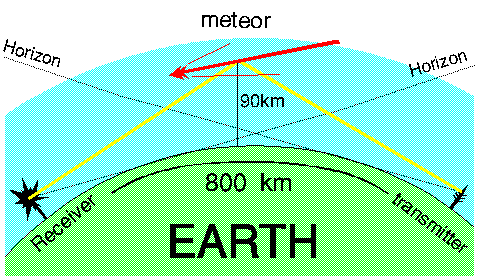
\includegraphics[width=\linewidth]{intro/detection}
	\caption{Diagram of forward scatter radio meteor detection (courtesy of \cite{forwardscatter})
		\label{fig:detection}}
\end{figure}\\
The transmitting antenna sends out a signal that reflects off of the ionised trail and is received by another station. The data that comes from detecting these ionised trails can be considered in various ways; most popularly by simply counting the number of detections an hour, or more visibly by displaying the intensity of the reflected signal for a range of frequencies against time. This produces a rather beautiful `waterfall' plot, seen in figure~\ref{fig:waterfall}. 
\begin{figure}[h!]
	\centering
	\begin{subfigure}{.24\textwidth}
		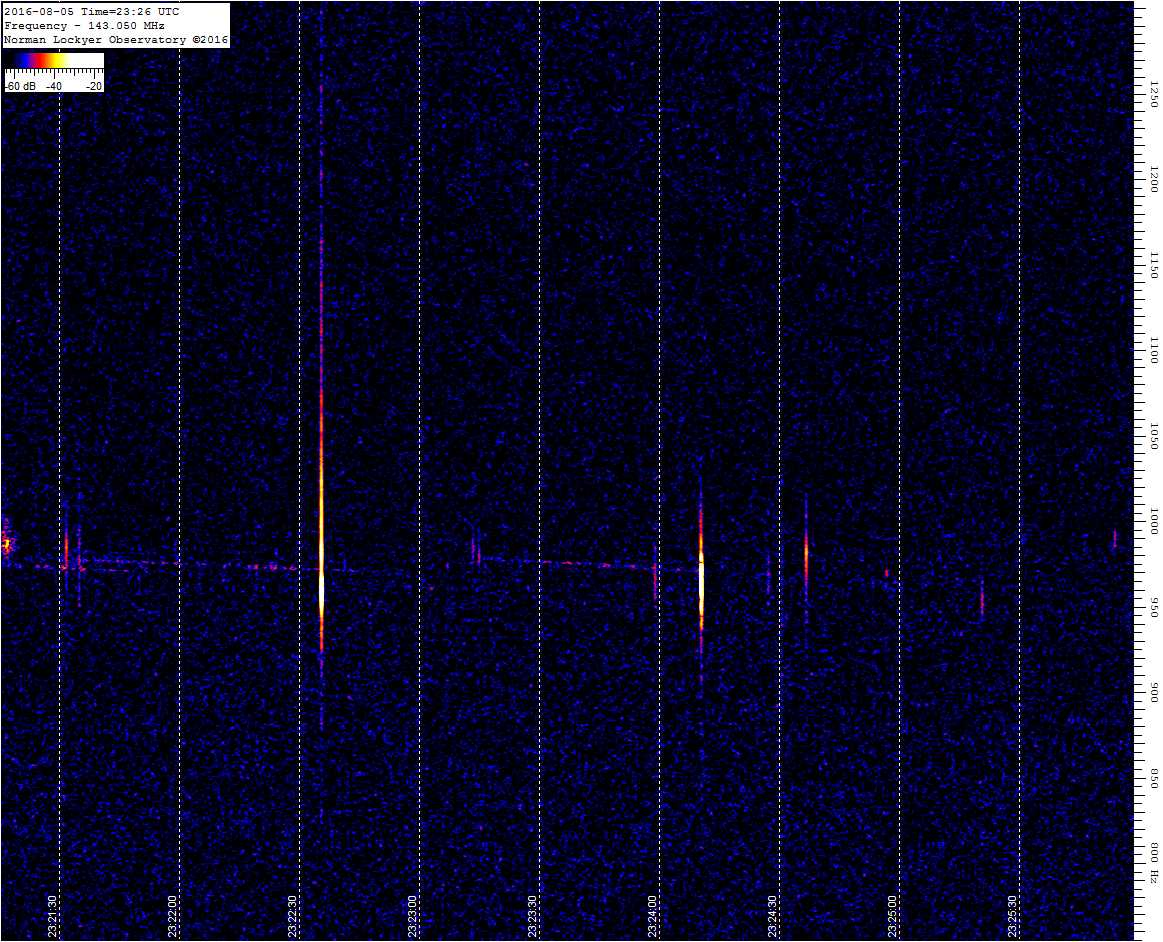
\includegraphics[width=\textwidth]{intro/2D}
		\caption{2D\label{fig:waterfall:a}}
	\end{subfigure}
	\begin{subfigure}{.24\textwidth}
		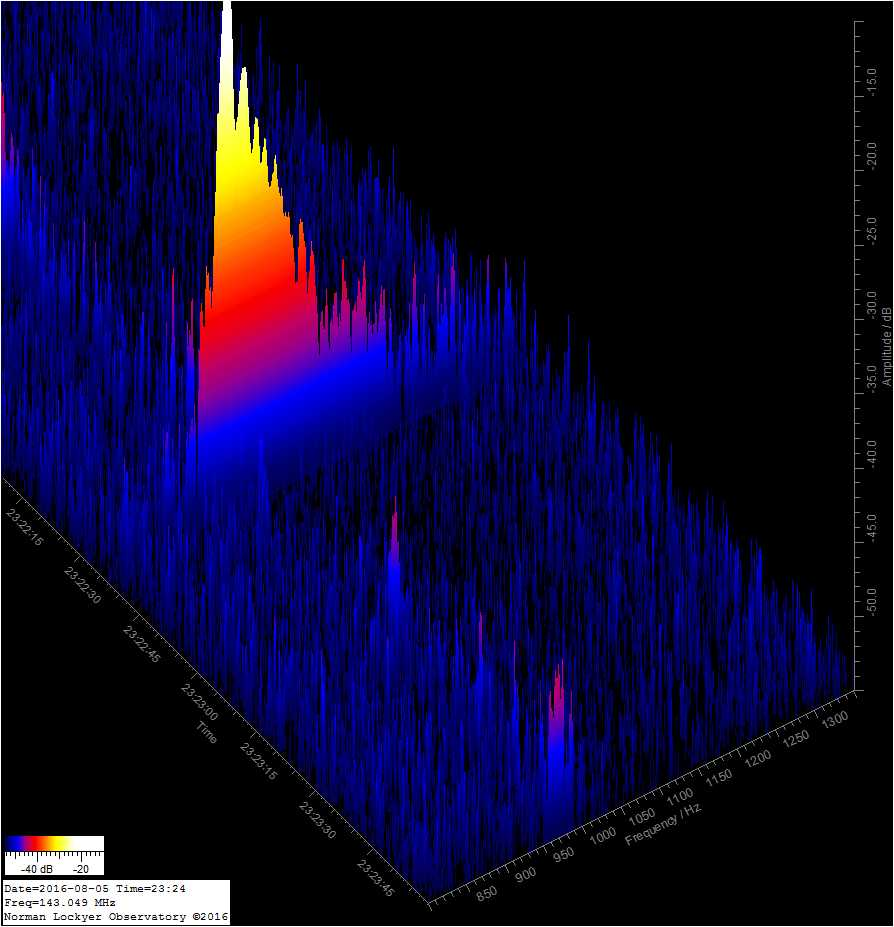
\includegraphics[width=\textwidth]{intro/3D}
		\caption{3D \label{fig:waterfall:b}}
	\end{subfigure}
	\caption{Waterfall plot 
	\label{fig:waterfall}}
\end{figure}\\
The `echo' received from the meteor has a characteristics shape depending on whether upper sideband (USB) or lower sideband (LSB) is used. In figure~\ref{fig:waterfall:a}, USB is used, producing an echo that trails off to the right, and has a peak to the left. The colour of the peak indicates the intensity of the received echo. The blue noise surrounding the echo is radio noise.\\
The alternative method, counting the number of meteors detected in an hour, is discussed in chapter~\ref{chap:data}.

\subsection{Meteor showers}
Typically, visual observation of meteors is done during a meteor shower. This event is characterised by an increased number of meteors observed, that are not sporadic. Sporadic meteors are those that do not appear to come from a common source -- they are simply debris entering the Earth's atmosphere. During a meteor shower, many more meteors are observed than normal, and most importantly, they appear to come from a common source: the radiant. This is the {\it apparent} source of all the shower meteors, that is, the meteors appear to travel out in all directions from this point.\\
The cause of a meteor shower is the Earth passing through the trail of debris left by a comet: dirty snowballs (figure~\ref{stream}). The only (notable) exception to this is the Geminids shower, which is caused by a Palladian asteroid rather than a comet's trail \cite{palladian}. The debris can be produced in many different ways, either through water vapour drag \cite{watervapour} (cite Fred Whipple 1951), by which ice melts and drags sand and pebble sized debris off the comet, or the breakup of parts of a comet.\\
\begin{figure}[h!]
	\centering
	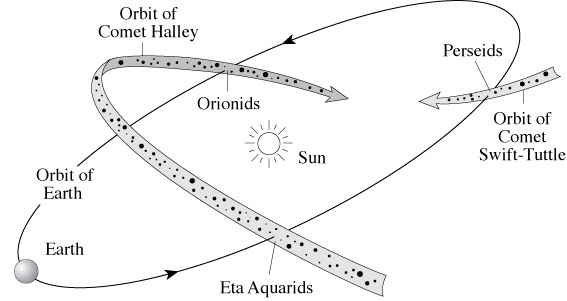
\includegraphics[width=\linewidth]{intro/stream}
	\caption{Meteor stream diagram (courtesy of \cite{stream})}
\end{figure}\\
As time passes, the stream will pass around the Sun and spread out. This means that, with time, a meteor shower's peak will become less pronounced as the meteoroids spread out across the entire orbit of the debris. However, showers caused by periodic comets will not suffer this effect since with each of the Comet's orbits, more debris is shed.\\
\begin{figure}
	\centering
	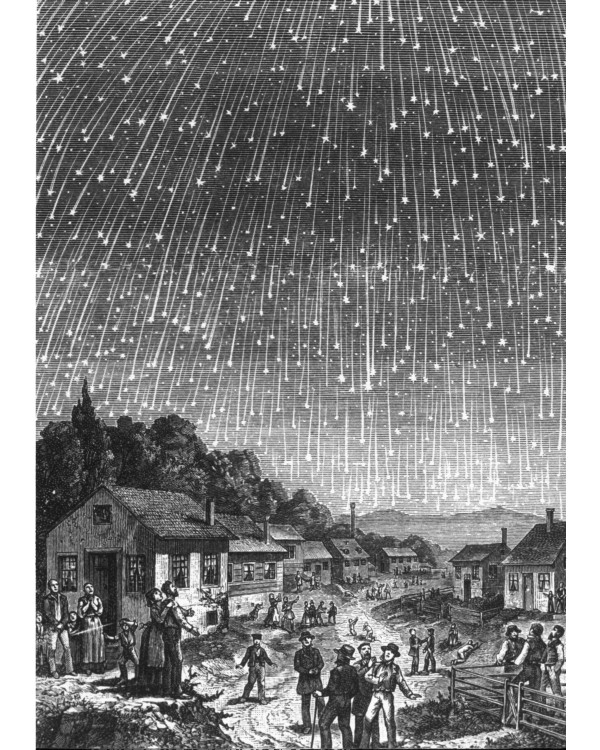
\includegraphics[width=0.8\linewidth]{intro/leonids}
	\caption{Leonids shower November 1833 (courtesy of \cite{leonids}) 
		\label{fig:1833leonids}}
\end{figure}\\
The most famous meteor showers include the Perseids, which often have the greatest number of meteors observed, which peak on the 12th or 13th of August. The Leonids originally gave birth to the name `meteor shower',  after a meteor `storm' in 1833 producing thousands of meteors a minute. (figure~\ref{fig:1833leonids}) This occurs once every 33 years (on average). Other showers, such as the Taurids, do not produce as many meteors, but are notable for frequent fireballs. These are meteors that explode due to the incredible pressure and heat of re-entry, and cause a sudden flash of light that can often illuminate the whole sky.


\subsection{Magnitude}
A measure of brightness (used throughout Astronomy) is magnitude. The magnitude scale is logarithmic and historically based around a single star, $\alpha$ Lyrae, which was used as the 0 point, though it is now defined in terms of flux. A decrease in magnitude by 1 means a brightness increase of $\sqrt[5]{100} \approx 2.512$. The larger the magnitude of a star, the fainter it is. Negative magnitudes are possible: for example, the Sun has an apparent magnitude of -27.\\
Apparent magnitudes are a measure of brightness from Earth, whilst absolute magnitudes are an objective measure of brightness, being the theoretical brightness of a star from a set distance (1 parsec). For visual observation (naked eye), meteors fainter than 6.5 in apparent magnitude cannot be seen. This is not the case for radio meteor detection.
\chapter{Data}
\label{chap:data}
\section{Where is the data from?}
The Radio Meteor Observing Bulletin (RMOB) \cite{rmob} is an organisation of people from the field of radio meteor scatter observations and data reduction. Started in August 1993, the intention was to enable easy communication of data from the Perseid meteor shower. In the years that followed the bulletin became monthly and now has hundreds of observers in various locations around the world. The long-term aim is to covert the {\it entire} world, allowing detection of stream outbursts that will not be noticed visually.\\
Pierre Terrier, an RMOB member, has produced software that allows observers to upload data to a database on the RMOB website (rmob.org). This is the source of my data, providing a range of data dating back to 2000, from observers across the globe.
\section{What is the data?}
The data provided by RMOB is a text and image collection, as in figure~\ref{fig:data:rmob}.\\
\begin{figure}[h!]
	\centering
	\begin{subfigure}{0.475\textwidth}
		\centering
		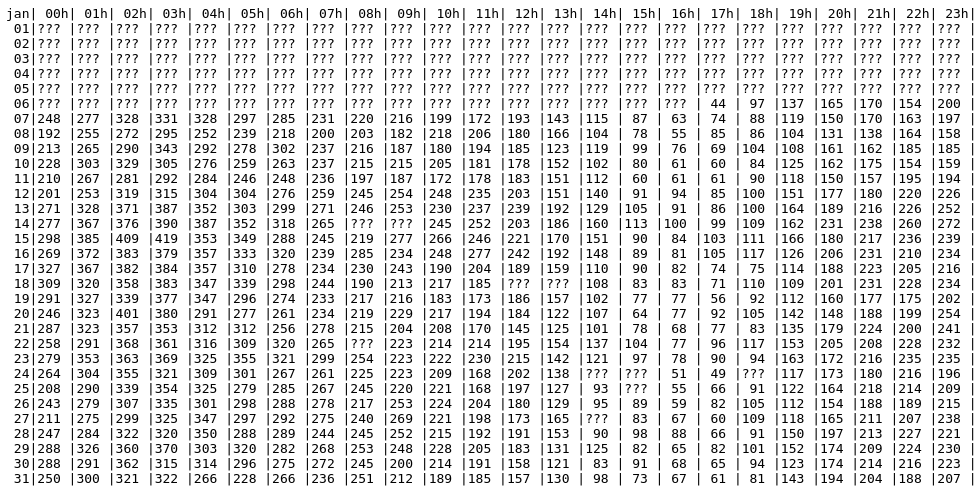
\includegraphics[width=0.9\linewidth]{data/rmob}
		\caption{Text format}
		\label{fig:data:rmob:a}
	\end{subfigure}
	\centering
	\begin{subfigure}{0.475\textwidth}
		\centering
		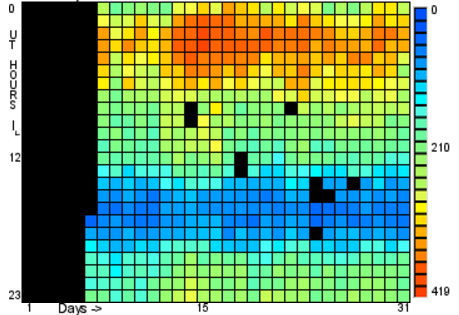
\includegraphics[width=0.9\linewidth]{data/rmob2}
		\caption{Image format}
		\label{fig:data:rmob:b}
	\end{subfigure}
	\caption{RMOB data formats
		\label{fig:data:rmob}}
\end{figure}
The data is collected using the observer's own radio setup. This will include an antenna, and a way of getting the signal to the computer. Typically this is done using a receiver (to control properties of the signal such as squelch) which feeds into the audio port of a computer or laptop. The software works in two parts. \\
The first stage is detecting the meteors from the signal. This is done using HROFFT \cite{hrofft} (figure~\ref{fig:data:hrofft}). 
\begin{figure}[h!]
	\centering
	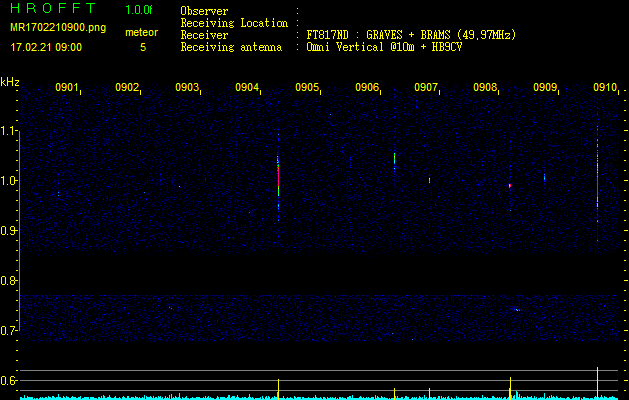
\includegraphics[width=\linewidth]{data/hrofft}
	\caption{HROFFT software screen (courtesy of \cite{hrofftimg})
		\label{fig:data:hrofft}}
\end{figure}\\
As can be seen in figure~\ref{fig:data:hrofft}, the intensity of the signal is calculated and shown in a light blue colour. The full waterfall plot is shown above this, making up the main part of the screen, much the same as figure~\ref{fig:data:rmob:b}. When the intensity of the signal goes over a threshold, it is noted as a meteor (yellow spike). The first threshold is 25dB, the second is 50dB and the third is 75dB. This information is then passed onto Colorgramme Lab. \\
In Colorgramme Lab, the counts are converted to text format and stored as seen in figure~\ref{fig:data:rmob:a}. At the end of the month, this data is uploaded to RMOB.

\section{Data collection \& storage}
\paragraph{Collection\\}
I have collected the data using webscraping. This is a process where a program (mine is written in Python) goes to a webpage, finds all the links on the page, and returns them. By going through each page of data available on the website, I could then download each text file, for each observer, for each month, for each year.\\
\paragraph{Storage\\}
I created two `objects' in Python in order to store the data. Objects are similar to real life objects -- self-contained elements that have their own properties. In the case of the RMOB data, it can be easily split into observers (the stations or people detecting the meteors) and `entries': monthly collections of data (a single text file from RMOB).\\
Using the links collected from webscraping, each file was downloaded, formatted,  and loaded into an entry. The data is not stored as part of the entry: the formatted file is saved to a folder. The formatting itself is so that the data is easy to use. Instead of storing the counts using `` | '' to separate the hours, I am using simple commas (``,'') to separate the hours. Instead of using ``???'' to denote unavailable data, I am using ``-1''. This makes it easier both to load the data, and to remove empty data.\\
Each entry has properties: the source of the data (the location in my filesystem that the data is stored), the date (in the format YYYY-MM) and the data itself. Storing every single item of data would be inefficient, so the data must be loaded through by typing \texttt{entry.loadData()} first. This opens the location in my filesystem, loads the .csv file, and the data is then available for processing. \\
Each of these entries is stored in an `observer' object. This is done by storing the entries in a dictionary, so that the correct data can be selected by specifying the month which is associated with the month of the entry. Some RMOB text files include properties of the detection setup, such as antenna, location, and frequencies. These are stored as part of the observer object as attributes. This allows an easier analysis, since in (for example) spatial variation, the GMAP location can be selected by typing \texttt{observer.locationAttr[`latitudeGMAP']}. Where two entries for the same observer differ, there is a `collision'. In this event, two separate observers are stored.
\section{Final data set}
Figure~\ref{fig:data:contr} shows how many observers contributed to RMOB each month since 2000. Overall, there are 345 observers in my data set, with 5110 entries in total. This means, at most, I have 3,800,000 hourly counts. As can be seen in the figure, more and more observers are uploading each month. This can only mean good things for meteor detection analysis!
\begin{figure}[h!]
	\centering
	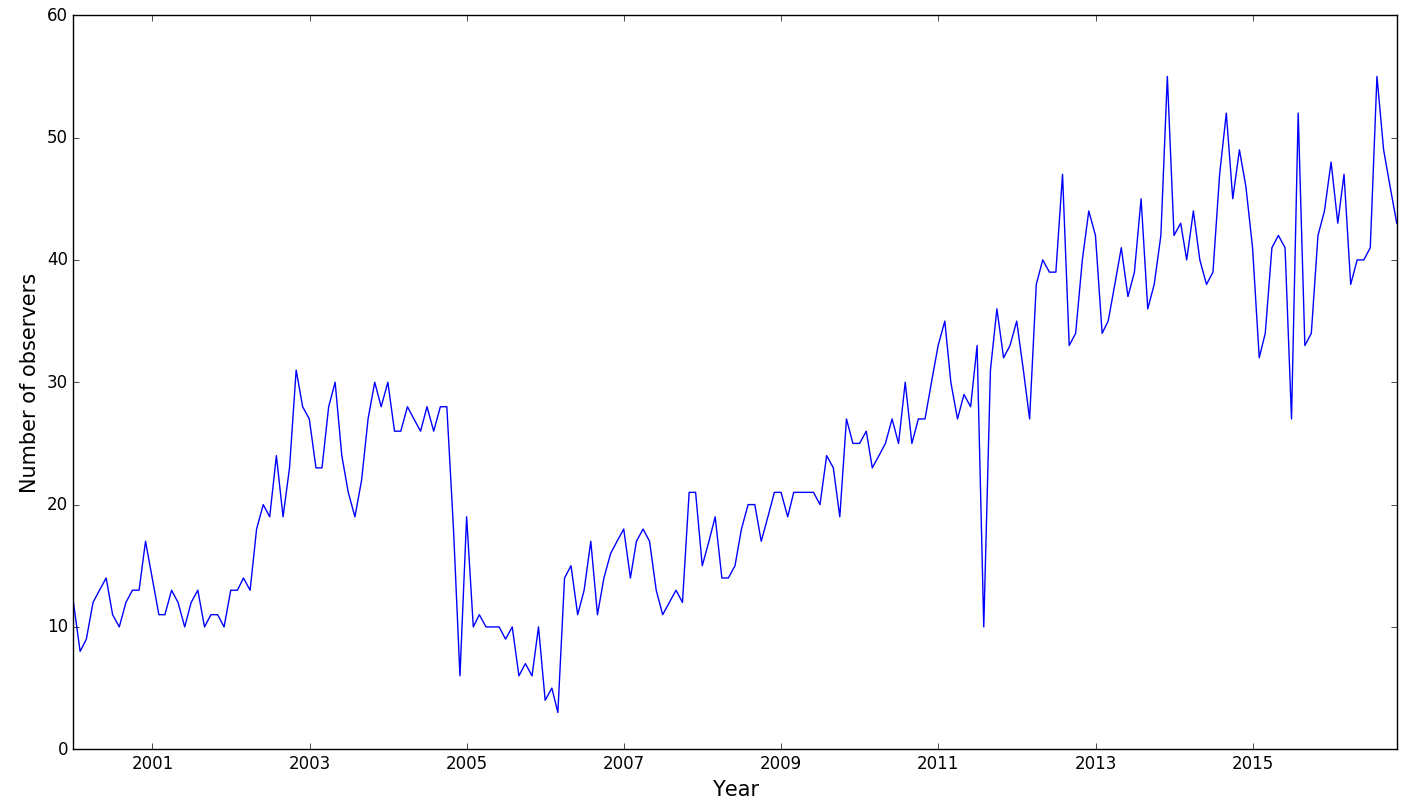
\includegraphics[width=\linewidth]{data/contributing_authors}
	\caption{Number of observers contributing each month
		\label{fig:data:contr}}
\end{figure}\\
Figure~\ref{fig:data:loc} shows the locations available in the data set. There is clearly a wide variety of locations, across the globe, which will make an analysis of spatial variation valid and worthwhile. 
\begin{figure}[h!]
	\centering
	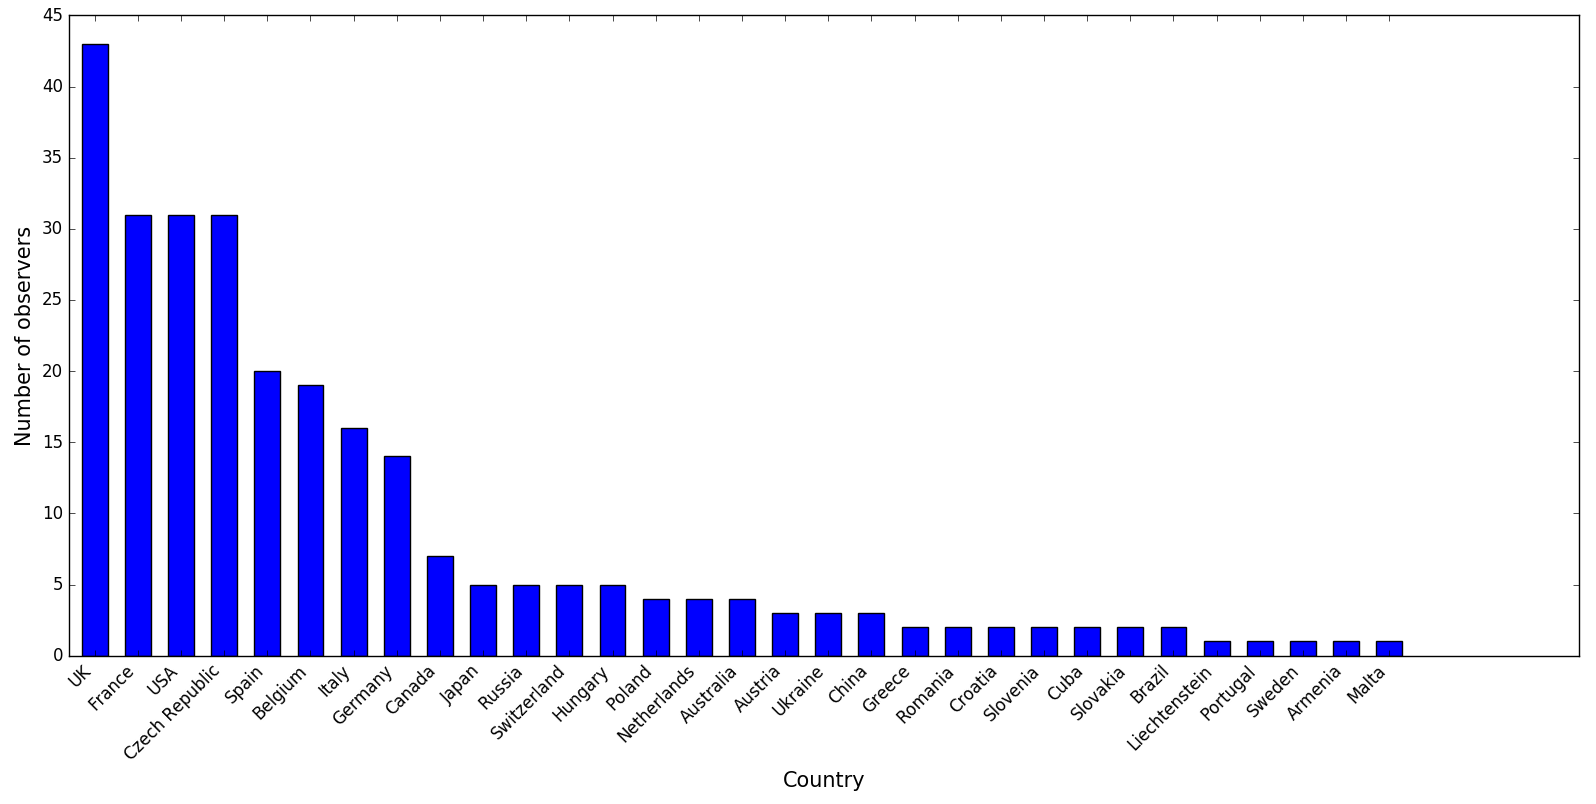
\includegraphics[width=\linewidth]{data/locations}
	\caption{Locations of observers (where known)
		\label{fig:data:loc}}
\end{figure}\\
Figures~\ref{fig:data:locvol} and \ref{fig:data:locavg} show the volume of data available for each country, and the average number of entries uploaded each month.
\begin{figure}[h!]
	\centering
	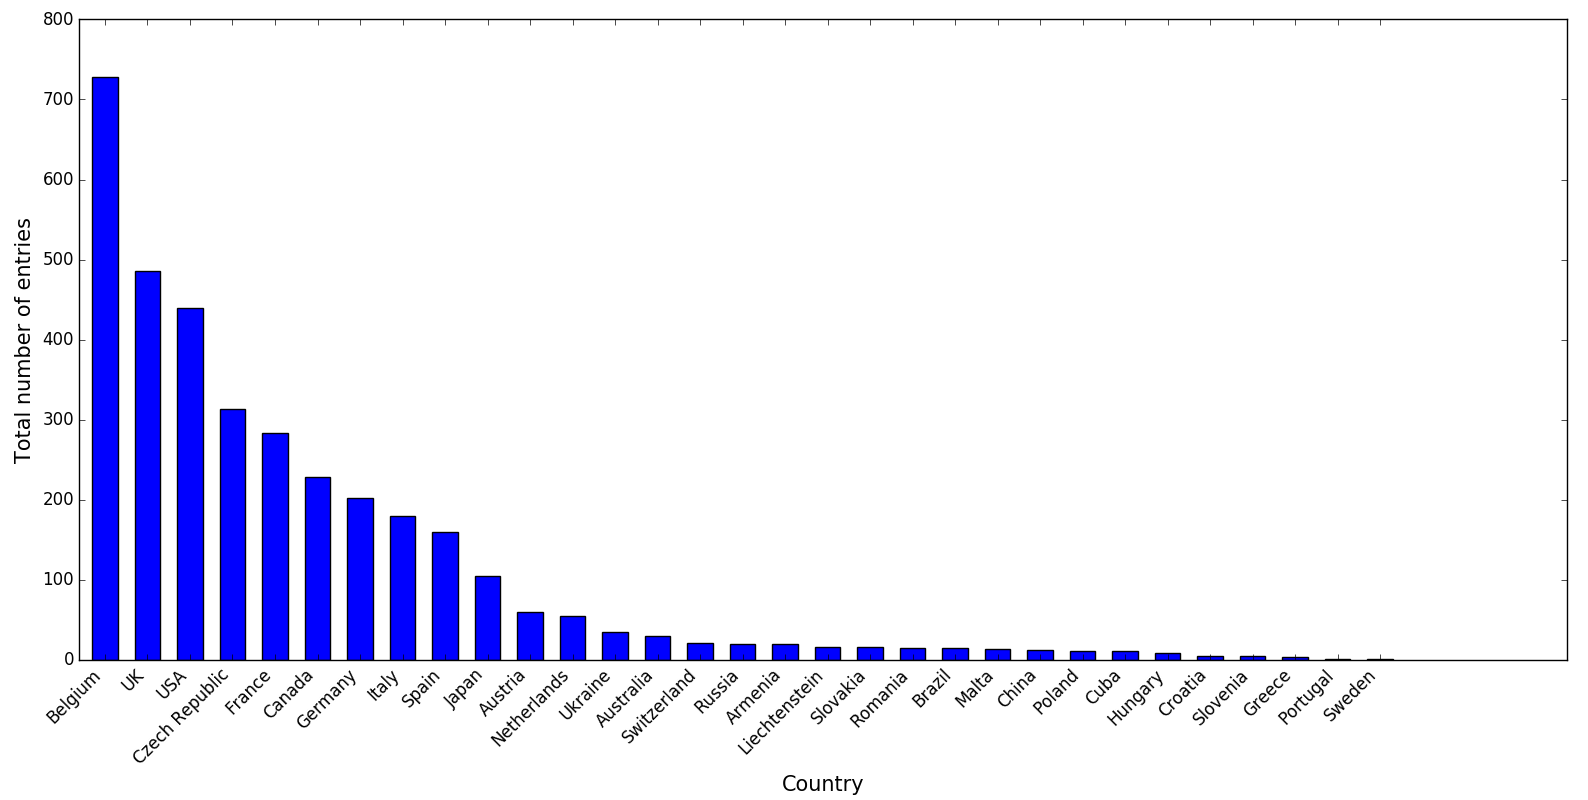
\includegraphics[width=\linewidth]{data/locationsVolume}
	\caption{Volume of data from each location (where known)
		\label{fig:data:locvol}}
\end{figure}
\begin{figure}[h!]
	\centering
	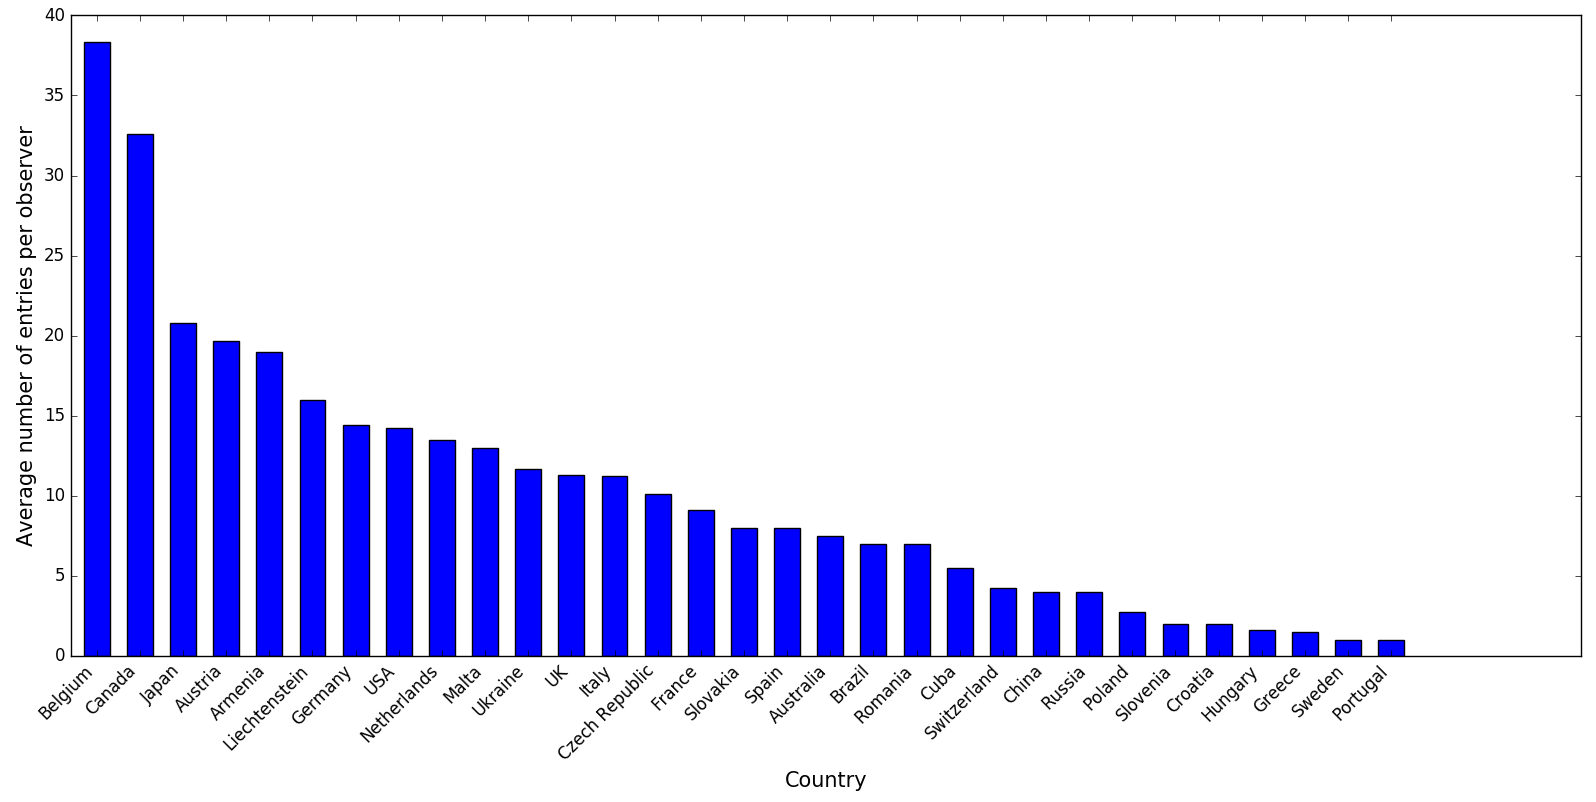
\includegraphics[width=\linewidth]{data/locationsAvg}
	\caption{Average number of entries per month from each location (where known)
		\label{fig:data:locavg}}
\end{figure}
\chapter{Diurnal Shift}
\label{chap:diurnalshift}
\begin{strip}
	\begin{minipage}{\textwidth}
		\begin{abstract}
			I present an improved model of diurnal shift, aiming to resolve issues evident in previous models and be more mathematically rigorous. I investigate the apparent sine-function variability of hourly meteor counts, as well as the temporal and spatial variation of said counts. My findings indicate that diurnal shift is dependent on Earth's orbital velocity, producing a clear trend between longitude and peak hour. I find no evidence of correlation between latitude and amplitude of diurnal variation.
		\end{abstract}
	\end{minipage}
\end{strip}
\section{Background}
For years, a notable increase and decrease over a single days' time scale has been observed in detection counts. An example of this is in figure~\ref{fig:data:rmob:b}. The red colours indicate a higher detection count, observed in the early hours of the morning. This diurnal shift {\it has} been given an explanation by modelling the phenomenon. The word `diurnal' refers to the time scale being a single day, and `shift' refers to the increase in detection counts. 
\section{Literature Review}
\subsection{Model}
Dr David Morgan of the BAA Radio Astronomy Group presents a somewhat detailed explanation \cite{baa} of why diurnal shift occurs. The suggestion is that diurnal shift is dependent on sporadic meteors rather than shower meteors, and depends on the variation of their intercept velocity with an observer on Earth. This changes since, as the Earth rotates, the combination of the orbital velocity, rotational velocity and meteor intercept velocity changes. As can be seen in figure~\ref{fig:dishift:model} (courtesy of the same article \cite{baa}), at Sunrise, the meteors velocity {\it adds} to Earth's orbital velocity, whilst at Sunset, these velocities {\it subtract}. 
\begin{figure}[h!]
	\centering
	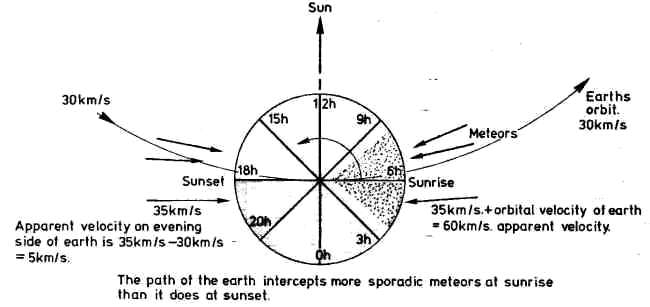
\includegraphics[width=\linewidth]{dishift/img59}
	\caption{Diurnal shift model
		\label{fig:dishift:model}}
\end{figure}
\subsection{Previous analyses}
\label{sec:dishift:litrev}
Diurnal variation is well studied. W. Singer, U. von Zahn and J. Wei{\ss} present an analysis \cite{alomar} of the diurnal and annual variations of meteor rates at the Arctic circle, specifically the ALOMAR observatory. They observe a clear diurnal shift, as well as an annual variation of this diurnal shift. The expectation that the intensity of the diurnal shift decreases towards the North Pole is not observed. \\
Singer, W., von Zahn, U., Batista, P. P., Fuller, B., \& Latteck, R. present an analysis \cite{latitudes} of the same subject that {\it does} observe an increase in diurnal shift intensity with decreasing latitude, which disagrees with the previous article \cite{alomar}. However, this analysis uses a wider range of latitudes to analyse, so the conclusion is likely more valid.
\section{Methodology}
In this analysis I will use previous results to examine spatial and temporal variation of diurnal shift, as well as how well a sine-function fits the diurnal shift curve.
The diurnal shift curve is generated by taking the mean of all data for a given hour after midnight, for each observer. Time, for all observers, is recorded in UTC. Using this curve I will compare the intensity of diurnal shift for three different location categories: Europe, Asia \& Australia, and North America. The sample sizes for each category are shown in table~\ref{tab:dishift:spatial}. In conjunction with this, I will fit a sine curve, to give an indication of a suitable function to describe the shift.
\begin{table}
	\begin{tabular}{cc}
		\hline
		Category & N$^{\circ}$ observers \\ \hline
		Europe & 220 \\
		Asia \& Australia & 12 \\
		North America & 37 \\
		\hline
	\end{tabular}
	\caption{Sample sizes for location categories
		\label{tab:dishift:spatial}}
\end{table}\\
\subsection{Spatial analysis}
I will use QGIS \cite{qgis} to generate a map, with a dot representing each observer with a known location. These dots will be coloured based on the peak hour of diurnal shift, indicating how this changes with location. Further to this, I will analyse the variation of the peak hour of diurnal shift, as well as the sum of parameter covariance for a sine function of the form $A \sin \left( \frac{2\pi}{24} t + \phi \right) + \mu$, indicating how well a sine curve fits the diurnal shift. This is calculated using a covariance matrix $M$, which gives the covariance of the parameter estimates as the sum of:
\begin{equation} 
\sum_{i=1}^3\left(\text{Diag}\left( M \right)_i \cdot \chi^2_{\text{residual}}\right)^{\frac{1}{2}}
\end{equation}\\
Here, $\chi^2_{\text{residual}} = \frac{X-x}{\sigma^2 (N-3)}$ where $N$ is the number of data points. 
This analysis will be over two independent variables: latitude and longitude. 
\subsection{Temporal analysis}
Finally I will analyse how the peak hour and parameter covariances vary over time, from 2000 to 2016. This will use the same calculated variables as the spatial analysis. These analyses will be completed using a Python program.

\section{Results \& Discussion}
\subsection{Model}
I aim to improve the model presented by Dr David Morgan \cite{baa}.
\paragraph{Inaccuracies\\}
The diagram and explanation have a few issues. Firstly, the diagram states (in conjunction with the explanation) that the path of the Earth intercepts more meteors at sunrise than sunset, causing the increase. This is not the case: the path of the Earth does not change, nor does the number of meteors being intercepted. What changes is the number of meteors that are intercepted that can be detected by a given observer. The explanation is suitable, but only if the cause is more rigorously explained as the velocity being proportional to the number of detections. When there is a greater velocity, more meteors can actually reach the Earth's atmosphere and be detected. \\
This is where the explanation appears to fall down. The diagram shows meteors intercepting the Earth at Sunset, and Sunrise, but nothing in between. Perhaps this is an ambiguity, but the implication is that there is a sudden increase and decrease. As is clear from the results, this isn't the case. The increase fits a sine curve remarkably well and the change occurs throughout the day. This suggests that the change, whilst it is indeed dependent on meteor intercepts, is a function applied to meteor velocities that is based on the angle of Earth's rotation. \\
\paragraph{Resolution\\}
\label{sec:dishift:model}
Building upon the previous model, I assume that the number of meteors detected is proportional to the mean incident velocity of meteors to Earth. This is reasonable: the {\it actual} velocities are of course random. However, an overall larger mean incident velocity of a collection of meteors means that proportionally more will reach Earth, of those that are in a direction that {\it could} cause a collision with Earth's atmosphere. Of a group of meteors with random velocities (both random magnitude {\it and} direction), very few will be on a course tangential to Earth's atmosphere. However, this does not change as Earth rotates, so it is a negligible variable. I consider only those that are tangential with the atmosphere, and so only those that could cause a detection. Thus, we have, at a very basic level:
\begin{equation}
N \propto v_{\text{incident}} 
\end{equation}
The incident velocity is dependent on factors such as the Earth's rotational velocity, orbital velocity and the velocity of the sporadic meteors themselves. $v_{\text{meteor}}$ is difficult to consider, since it (theoretically) has a random direction. We know that $v_{\text{orbit}} \approx 30000 \, ms^{-1}$ and  $v_{\text{rotation}} \approx 450 \, ms^{-1}$.\\
Assuming that the path described by Earth's orbit around the Sun is a straight line through Earth when `up close', let $\theta$ be the angle between a radius from the Earth's centre to the observer's location, and the orbital path (figure~\ref{fig:dishift:ownmodel}). The set of meteors that can be detected appear, from above, to form a triangle. The average velocity of these meteors will be along the height of this triangle: perpendicular to the surface of Earth. This means that the rotation velocity can be disregarded. Thus, the remaining velocity to consider is Earth's rotational velocity:
\begin{equation}
v_{\text{incident}} = v_{\text{orbit}} \cos \theta + v_{\text{meteor}}
\end{equation}
Clearly, this is at a maximum when $\theta = 0^{\circ}$. For an observer at a longitude of $0^{\circ}$, this is 6am. Since this is where the angle is defined from, it is clear that for any observer the peak hour will be 6am local time (assuming local time is based off of longitude, not timezones). It should be noted that the peak hour can vary around this time, based on conditions for observing. Particularly important are changes in the ionosphere as the Sun rises, allowing better reception of signals from transmitting antennas, providing better conditions for radio meteor detection. This could slightly shift the peak hour to be later than 6am.

\subsection{Sine-function fit}
Figure~\ref{fig:dishift:fit} shows the results for a sine function fit. The optimal sine function and cubic are shown in red and green respectively.  The sum of the covariance for each parameter of the optimal sine curve (of the form $A \sin \left( \omega t + \phi \right) + \mu$) is 0.814, which indicates a positive correlation. This suggests (as is clearly apparent from the figure) that the sine function fits well. As a reference, I fitted a cubic. This shows how well a sine curve fits in comparison. The implication of this is that the cause of diurnal shift is based on a sine function of the Earth's rotation (i.e. the hour of the day).

\begin{figure}[h!]
	\centering
	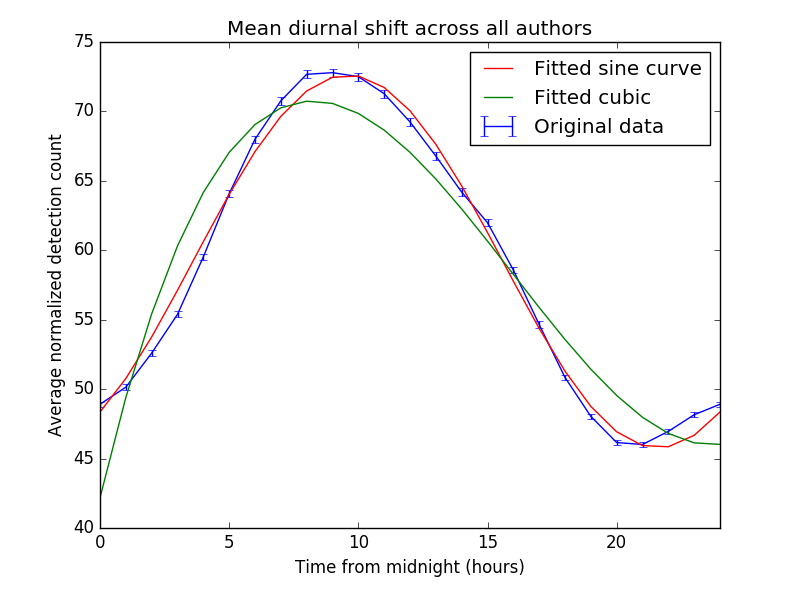
\includegraphics[width=\linewidth]{dishift/diurnal_shift_fit}
	\caption{Diurnal shift across all authors \& sine-function fit
		\label{fig:dishift:fit}}
\end{figure}

Figure~\ref{fig:dishift:all} shows the same graph as figure~\ref{fig:dishift:fit} (for comparison), as well as diurnal shift curves for each respective location. Surprisingly, each location category shows a sine curve. The peak of these sine curves appears to be correlated well with latitude. The average longitudes in degrees are, for Europe, Asia \& Australia, and North America respectively: $\sim 15$, $\sim 150$ \& $\sim -100$. This supports the idea of a sine-function describing the diurnal shift, since larger longitudes produce a greater hour of diurnal shift, bearing in mind that the hour for the North American categoryw ill `wrap' around, due to timezones. The average latitudes in degrees are (respectively): $\sim 45$, $\sim 35$ \& $\sim 15$. The North American category has the largest intensity, followed by the European category and then Asia \& Australia, though this is not the order of latitudes. This appears to disagree with research noted in section~\ref{sec:dishift:litrev}, which suggested that the intensity (amplitude) of diurnal shift is dependent on latitude.  

\begin{figure}[h!]
	\centering
	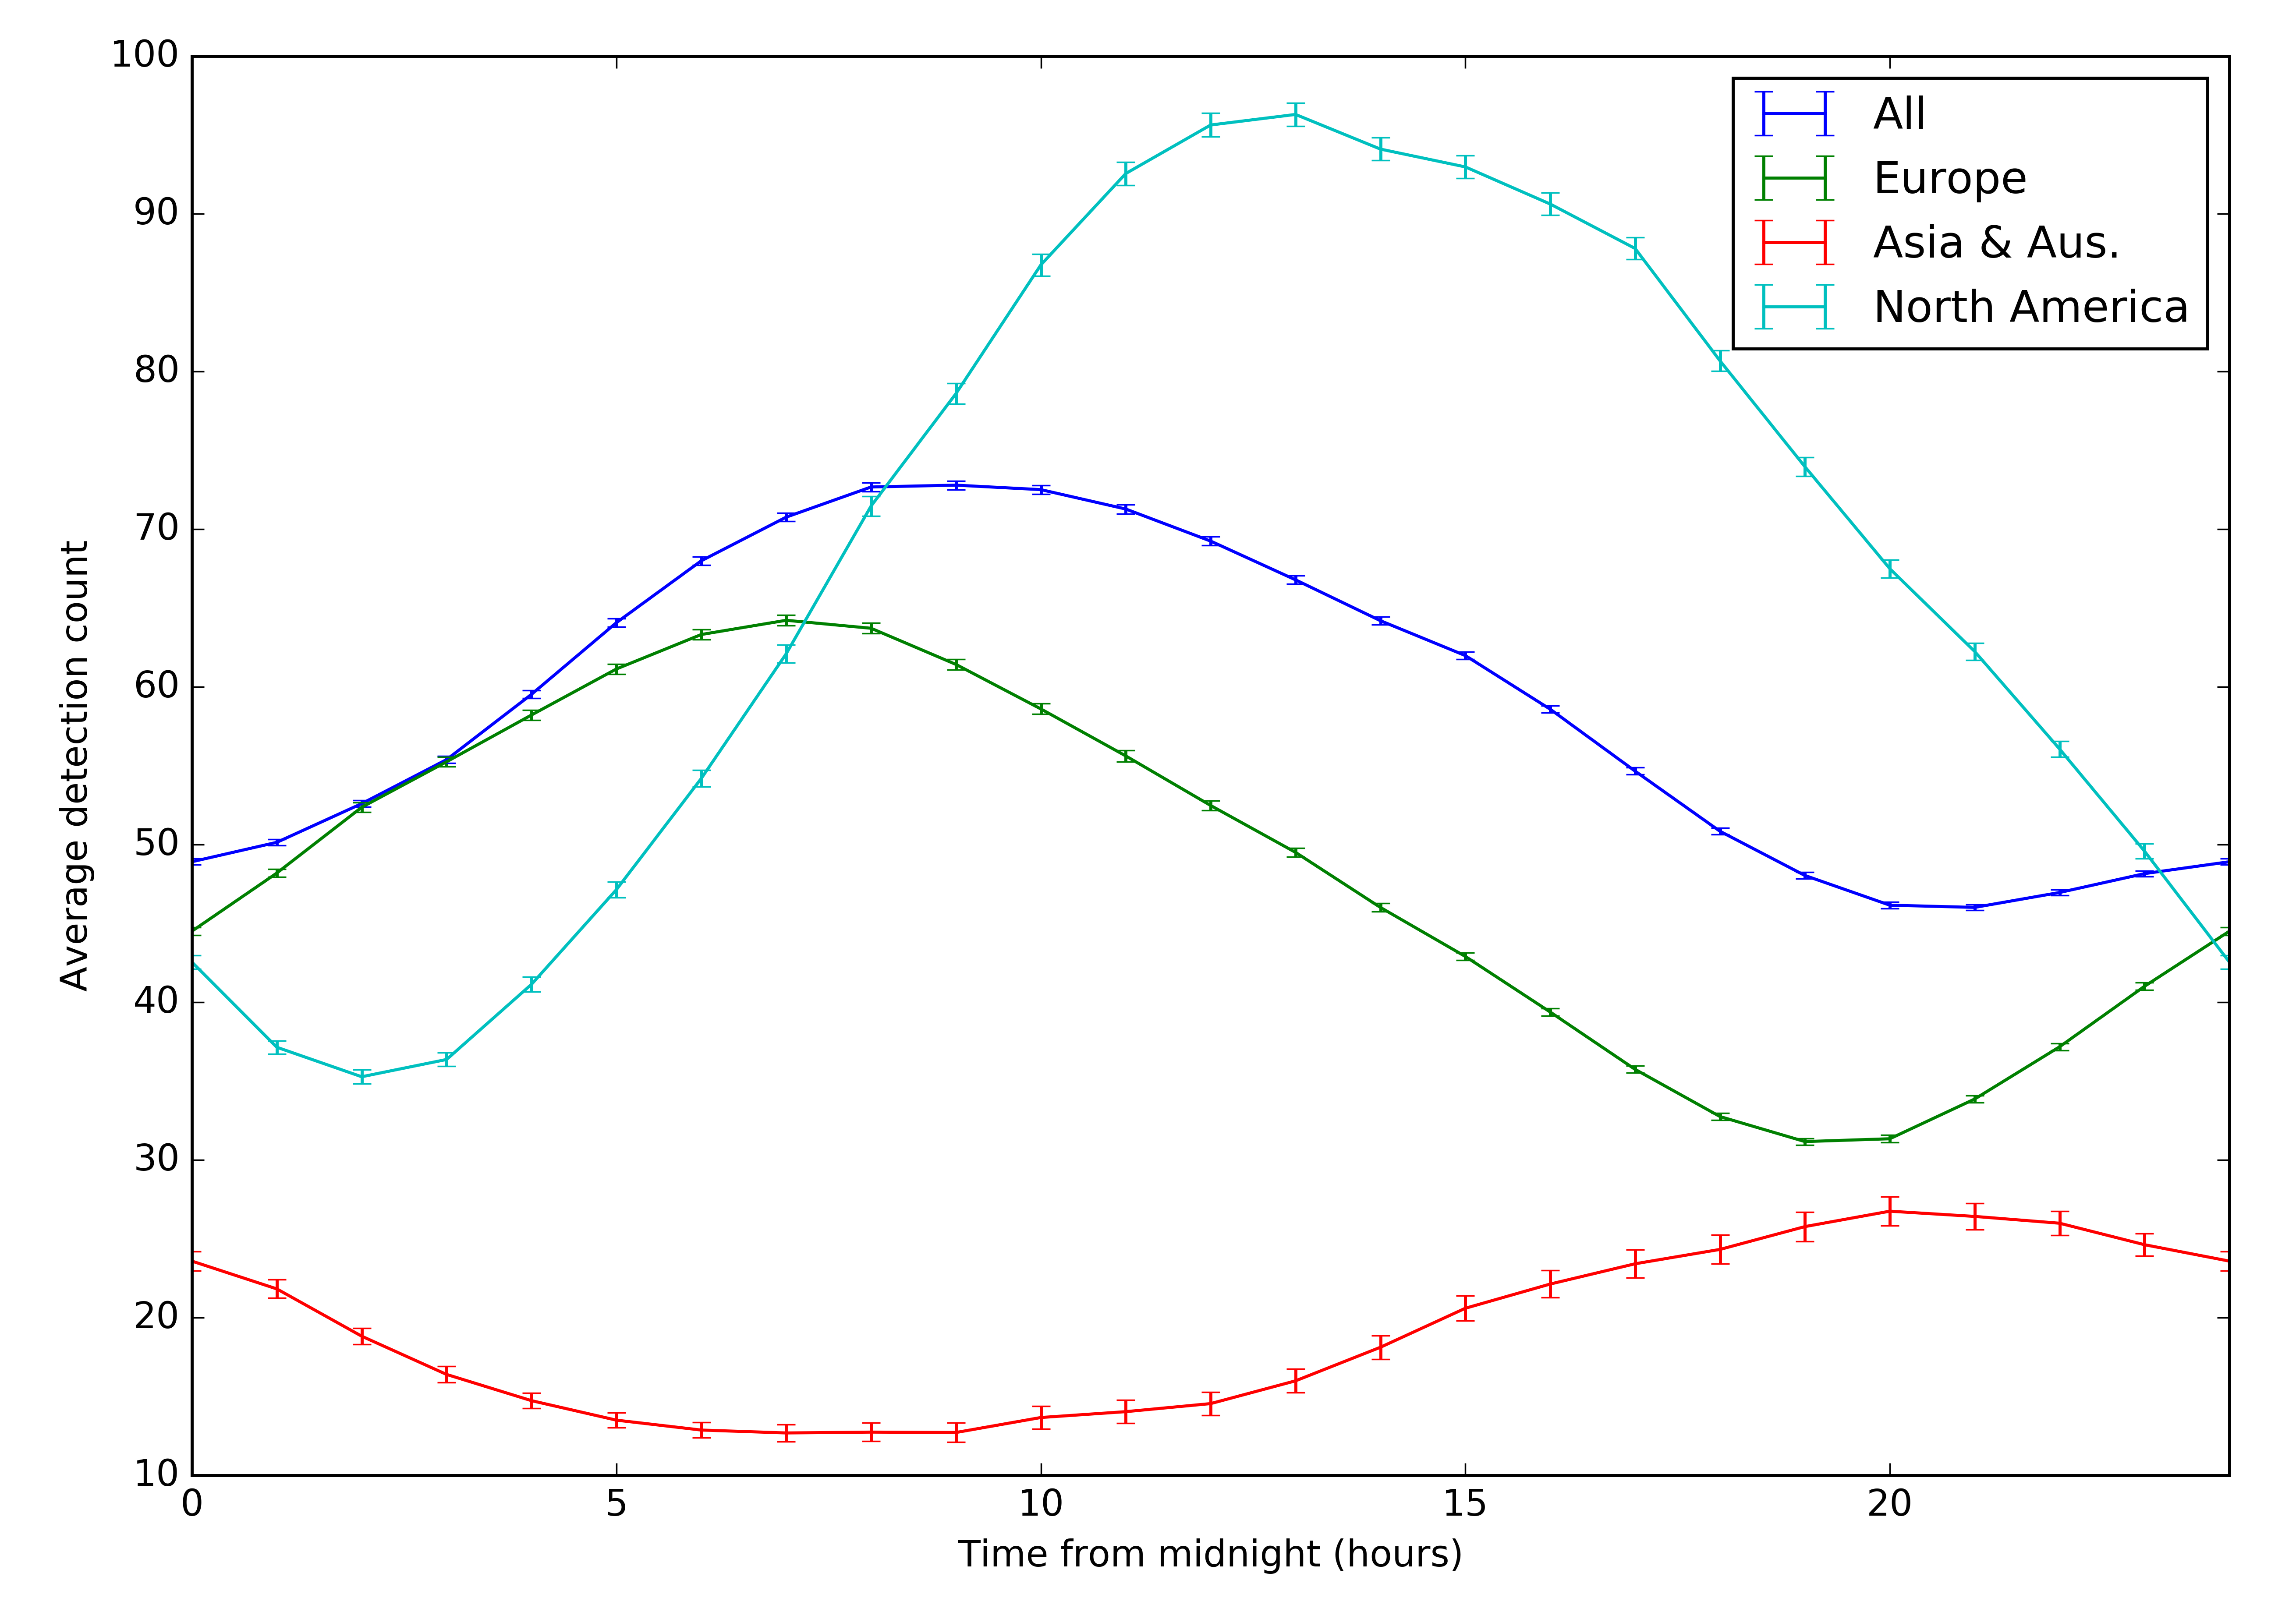
\includegraphics[width=\linewidth]{dishift/all_shifts}
	\caption{Diurnal shifts for each individual location (all observers' shift included for reference)
		\label{fig:dishift:all}}
\end{figure}

The sum of parameter covariances for each location category are shown below. The positive numbers all indicate a positive correlation, as expected from the figures. 
\begin{table}[h!]
	\begin{tabular}{ccccc}
		\hline
		Category & $A$ & $\phi$ & $\mu$ & Covar. \\ \hline
		All & 13.4 & -0.941 & 59.2 & 0.454 \\
		Europe & 15.4 & -0.302 & 48.4 & 0.498 \\
		Asia \& Aus. & -7.19 & -0.585 & 19.0 & 0.352 \\
		N. America & 29.5 & -2.05 & 68.1 & 1.16 \\
		\hline
	\end{tabular}
	\caption{Sum of parameter covariances for each location category}
\end{table}

\subsection{Spatial variation}
Created using QGIS, I present a map showing the location of each observer in the data set. The dot for each circle is coloured (as in the legend) based on the peak hour of the diurnal shift. This gives a more visual demonstration of what is shown in figures~\ref{fig:dishift:all} and \ref{fig:dishift:lon:peak}: the colours are clearly grouped based on location. Observers in Europe have diurnal shift peaks mostly around 6:00, North American observers have peaks around 15:00 and in Asia \& Australia around 20. This supports implications from the previously stated figures. There are clearly anomalous results for some observers (note the blue dots in Europe), though this is expected.
\begin{figure}[h!]
	\centering
	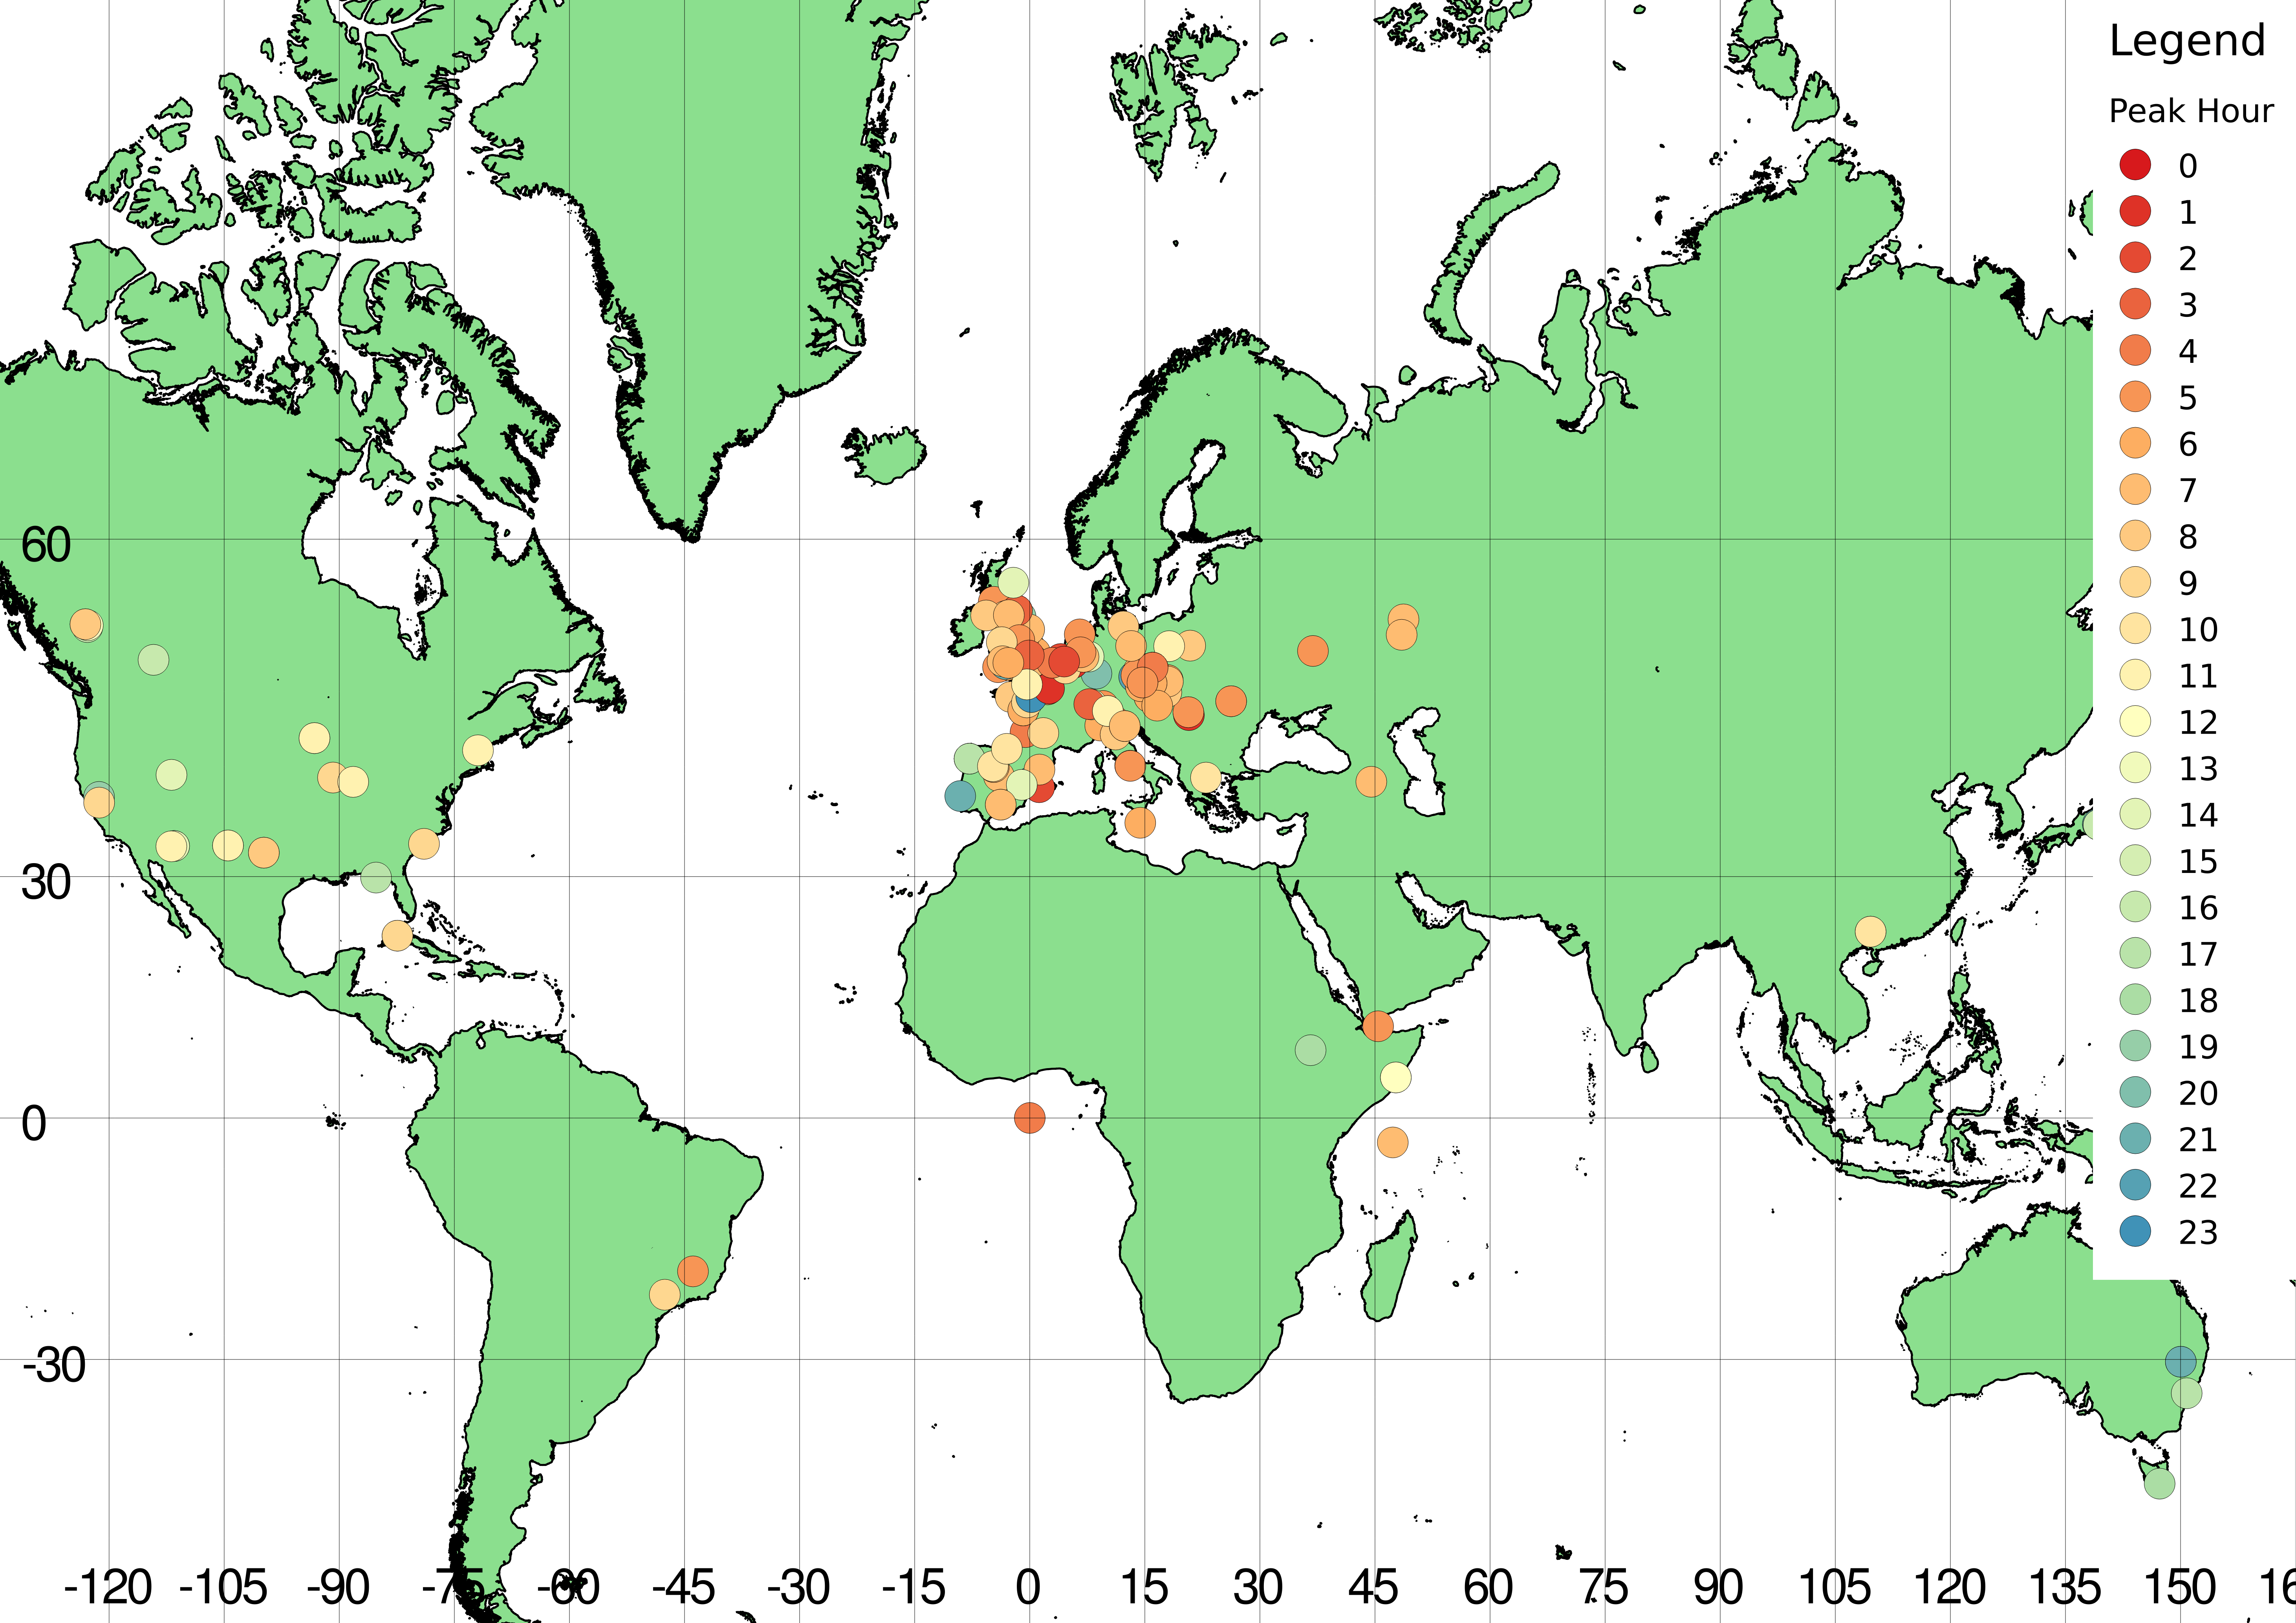
\includegraphics[width=\linewidth]{dishift/peak_qgis}
	\caption{Peak hour of diurnal shift for each observer
		\label{fig:dishift:qgis}}
\end{figure}
\paragraph{Latitude\\}
There appears to be little correlation between latitude and the peak hour. Although, overall, the hour appears to decrease as the latitude varies from $-40^{\circ}$ to $60^{\circ}$, there errors are substantial. The implication of this is there is little agreement within each category, suggesting no correlation at all. However, this is expected. There is no logical reason why the peak hour would be influenced by the latitude. Diurnal shift is caused (according to my model and \cite{baa}) by the Earth's rotation changing the average incident velocity of meteors. This does not change with latitude, hence no correlation is seen.
\begin{figure}[h!]
	\centering
	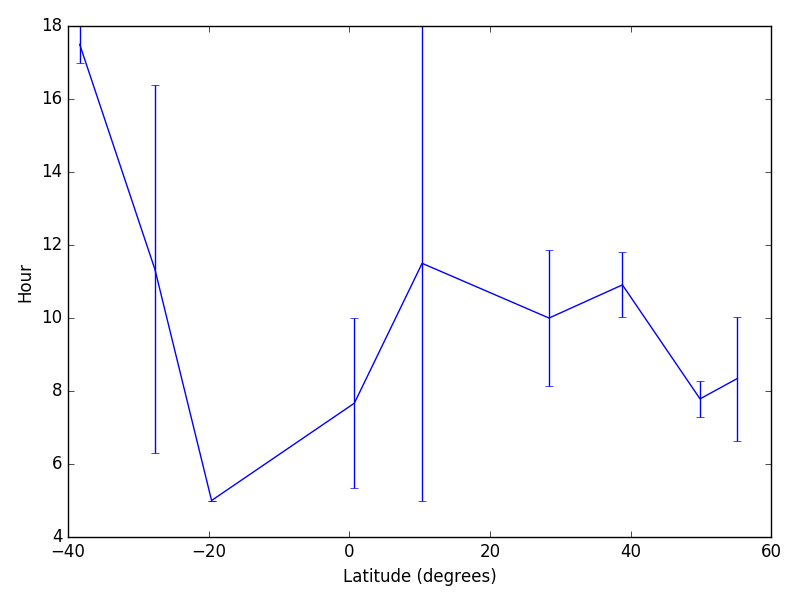
\includegraphics[width=\linewidth]{spatial/latitude/peak}
	\caption{Peak hour of diurnal shift against latitude
		\label{fig:dishift:lat:peak}}
\end{figure}

In figure~\ref{fig:dishift:lat:fit} little correlation is seen again. The covariances vary widely. There is no clear trend, suggesting that the latitude of an observer has no effect on how well data fits a sine function. Consequently, it would appear that diurnal shift is a global phenomenon.
\begin{figure}[h!]
	\centering
	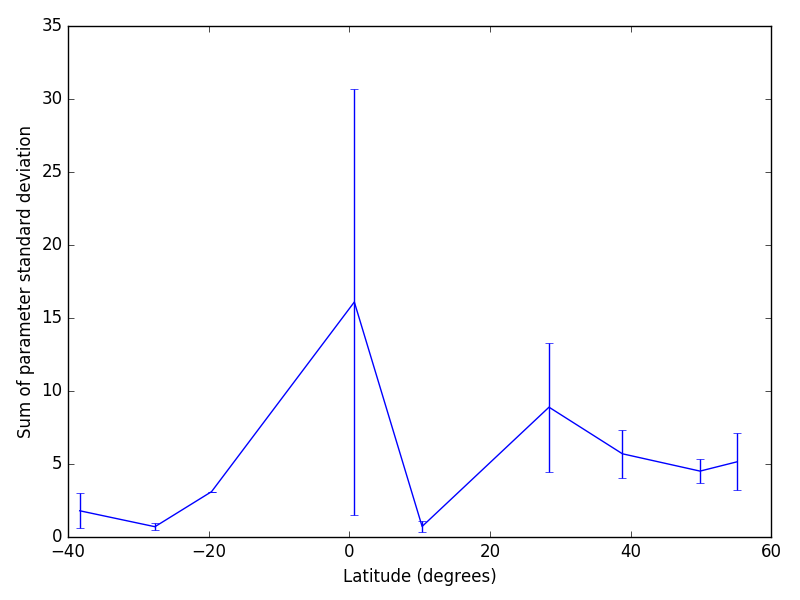
\includegraphics[width=\linewidth]{spatial/latitude/fit}
	\caption{Optimal sine function fit against latitude
		\label{fig:dishift:lat:fit}}
\end{figure}

\paragraph{Longitude\\}
Figure~\ref{fig:dishift:lon:peak} shows agreement with figures~\ref{fig:dishift:all} and \ref{fig:dishift:qgis}. The peak hour is lowest for a longitude of $0^{\circ}$ and increases either side of this, as seen in the stated figures. The errors for some categories are reasonably large, though still fall in a range that fits the trend. There is, of course, minor variation though the trend is clear from the data: latitude and peak hour of diurnal shift are related.
\begin{figure}[h!]
	\centering
	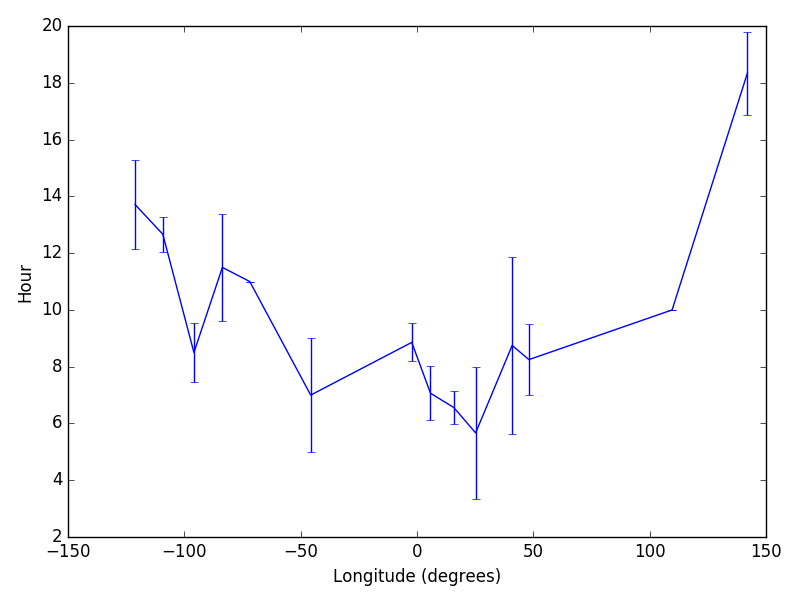
\includegraphics[width=\linewidth]{spatial/longitude/peak}
	\caption{Peak hour of diurnal shift against longitude
		\label{fig:dishift:lon:peak}}
\end{figure}\\
In order to investigate this apparent trend further, I have corrected the peak hour of each location category such that $H_{\text{corrected}} = H_{\text{calculated}} + \frac{\phi}{15}$, provided the longitude $\phi$ is in degrees. This means that the hour will be the local time (not using timezones, only the time based on longitude). This is shown in figure~\ref{fig:dishift:lon:corrected}. Errorbars, in this case, are such that 75\% of the data for a given location category falls within the bars. The values appear to fluctuate around a peak hour of 6am (shown in green), supporting the model I have proposed. However, there is a large degree of variation.
\begin{figure}[h!]
	\centering
	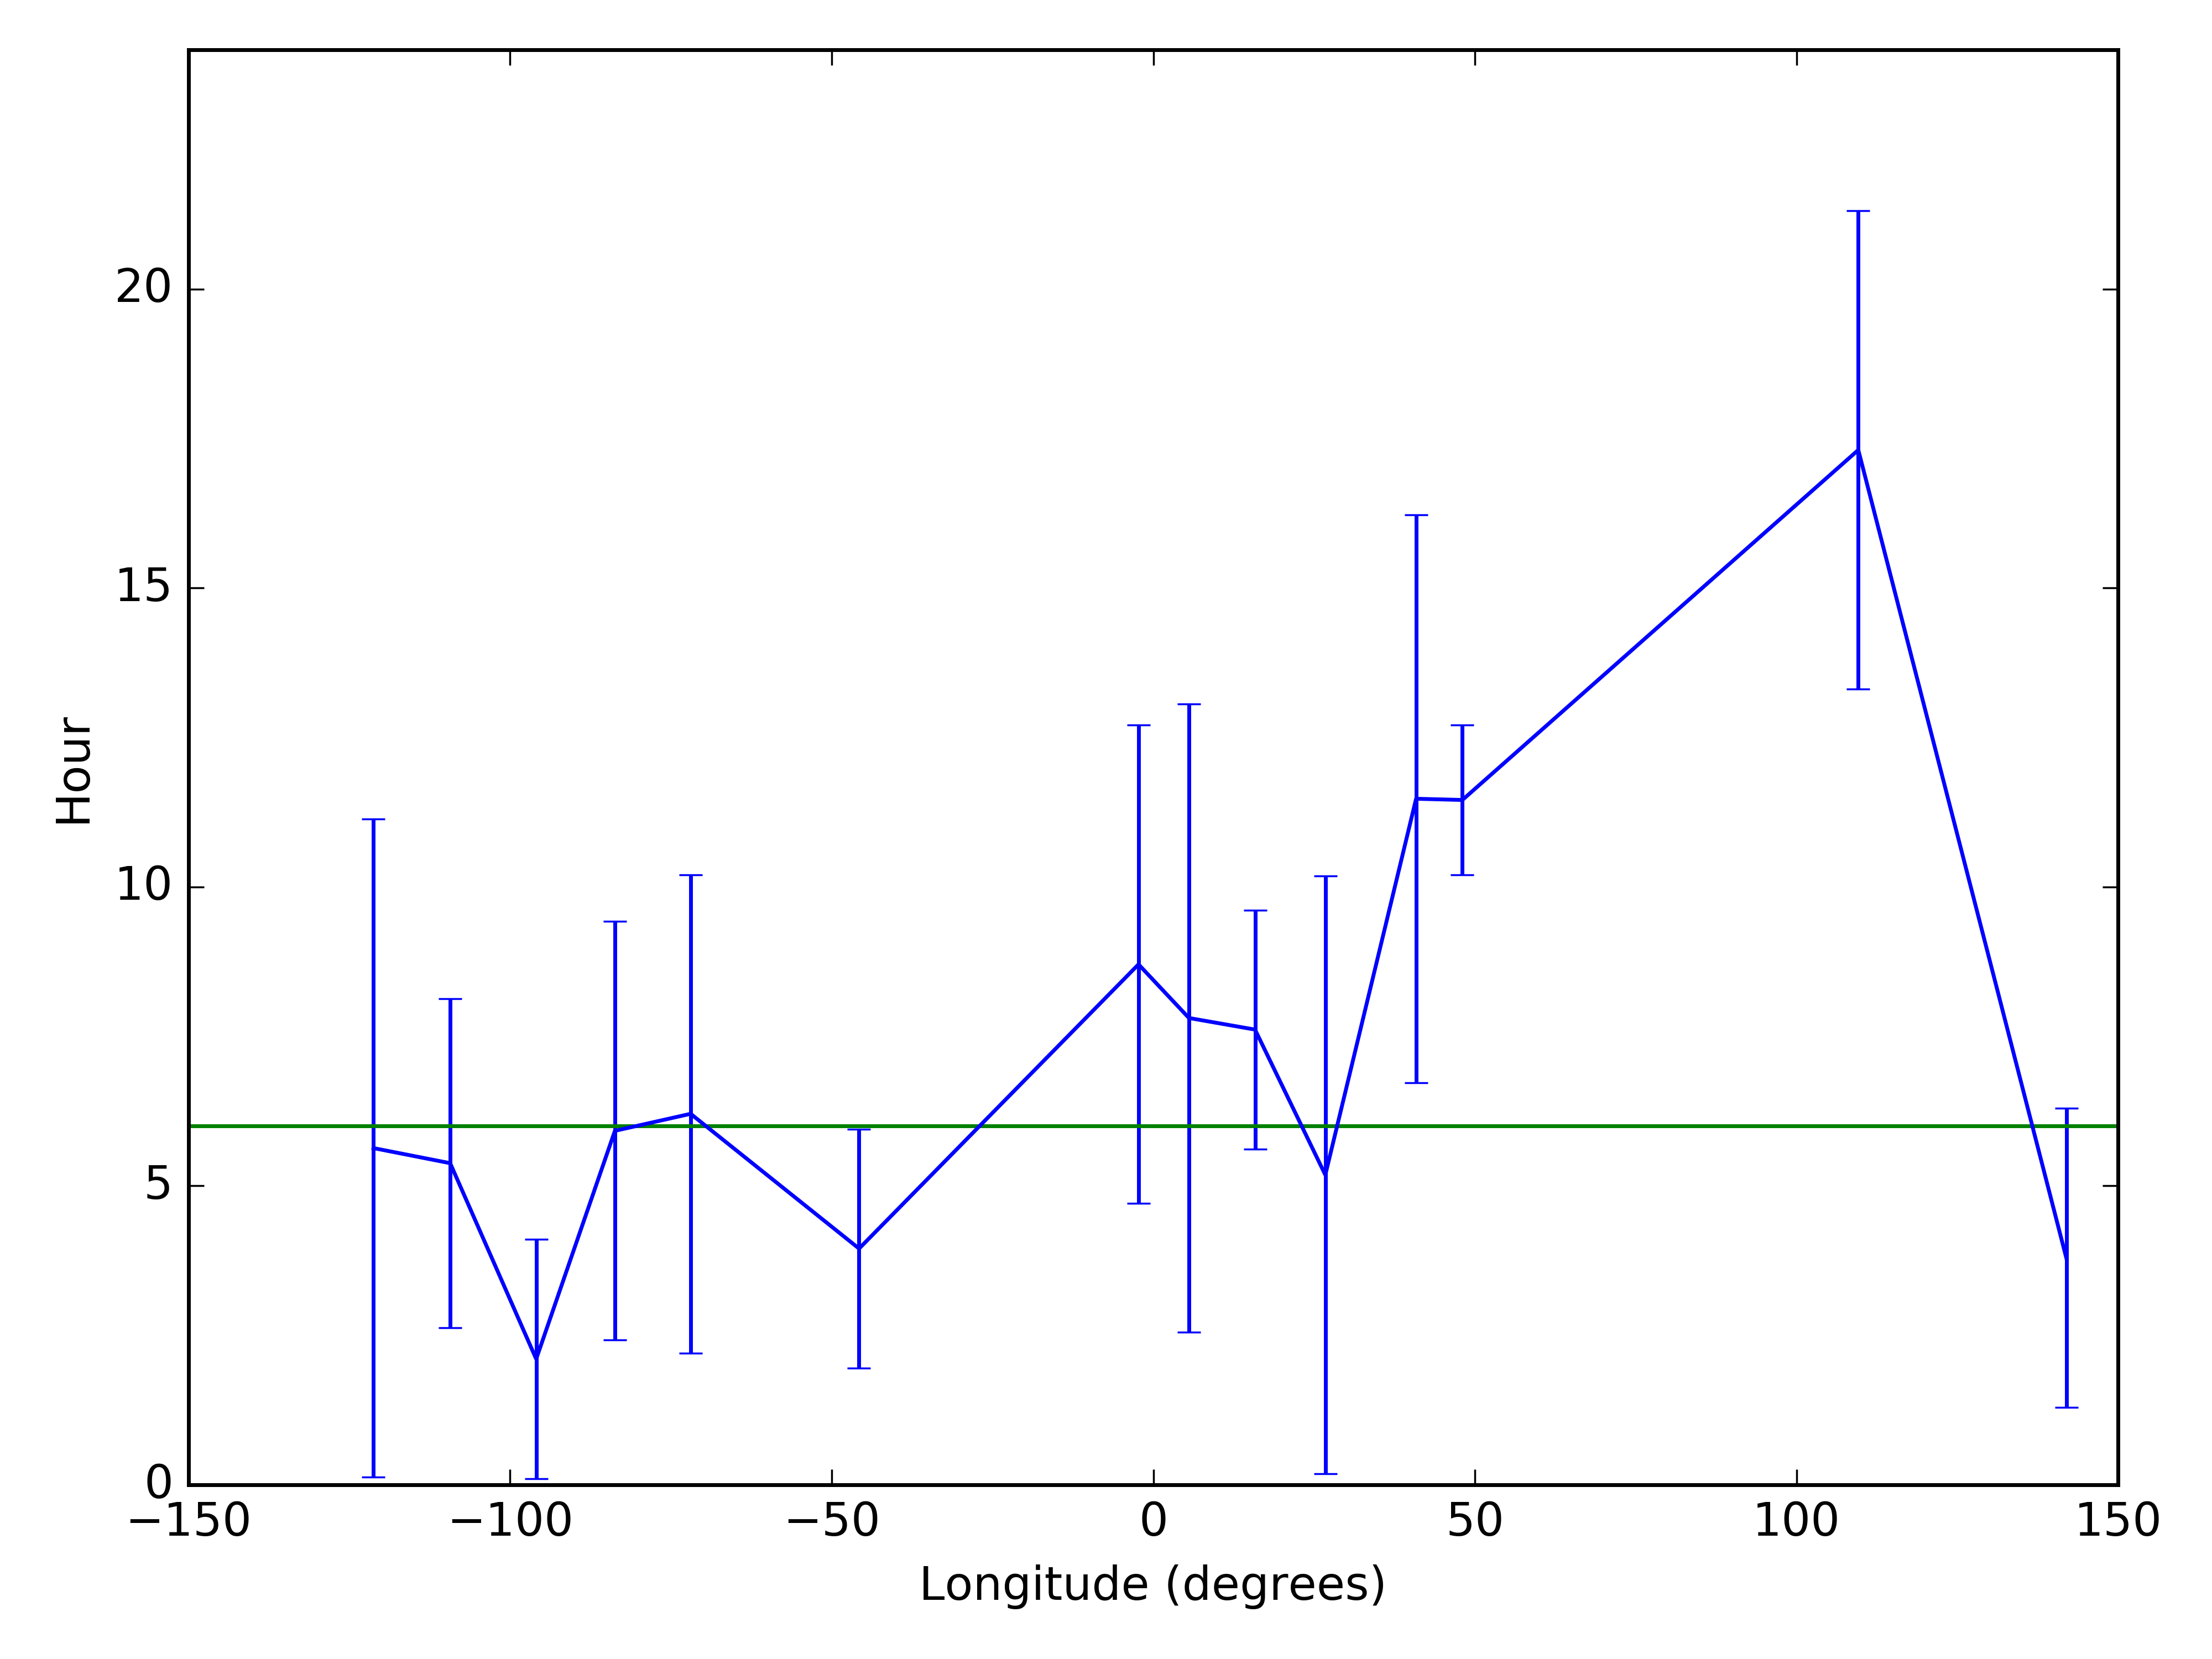
\includegraphics[width=\linewidth]{spatial/longitude/corrected}
	\caption{Corrected peak hour of diurnal shift against longitude
		\label{fig:dishift:lon:corrected}}
\end{figure}\\
In figure~\ref{fig:dishift:lon:hist} a histogram of the peak hour is shown. It is clear from this figure that the model is supported. Clearly most of the observers have a peak hour around 6, with some having a peak hour of 7. This is reasonable; as noted in section~\ref{sec:dishift:model}, the peak hour can in fact be slightly after 6am, since changes in the ionosphere occur around this time, as the Sun comes over the horizon. This can improve radio detection, allowing for better conditions that would shift the peak hour. Of course, there is some distribution either side of 6am, though this is expected.
\begin{figure}[h!]
	\centering
	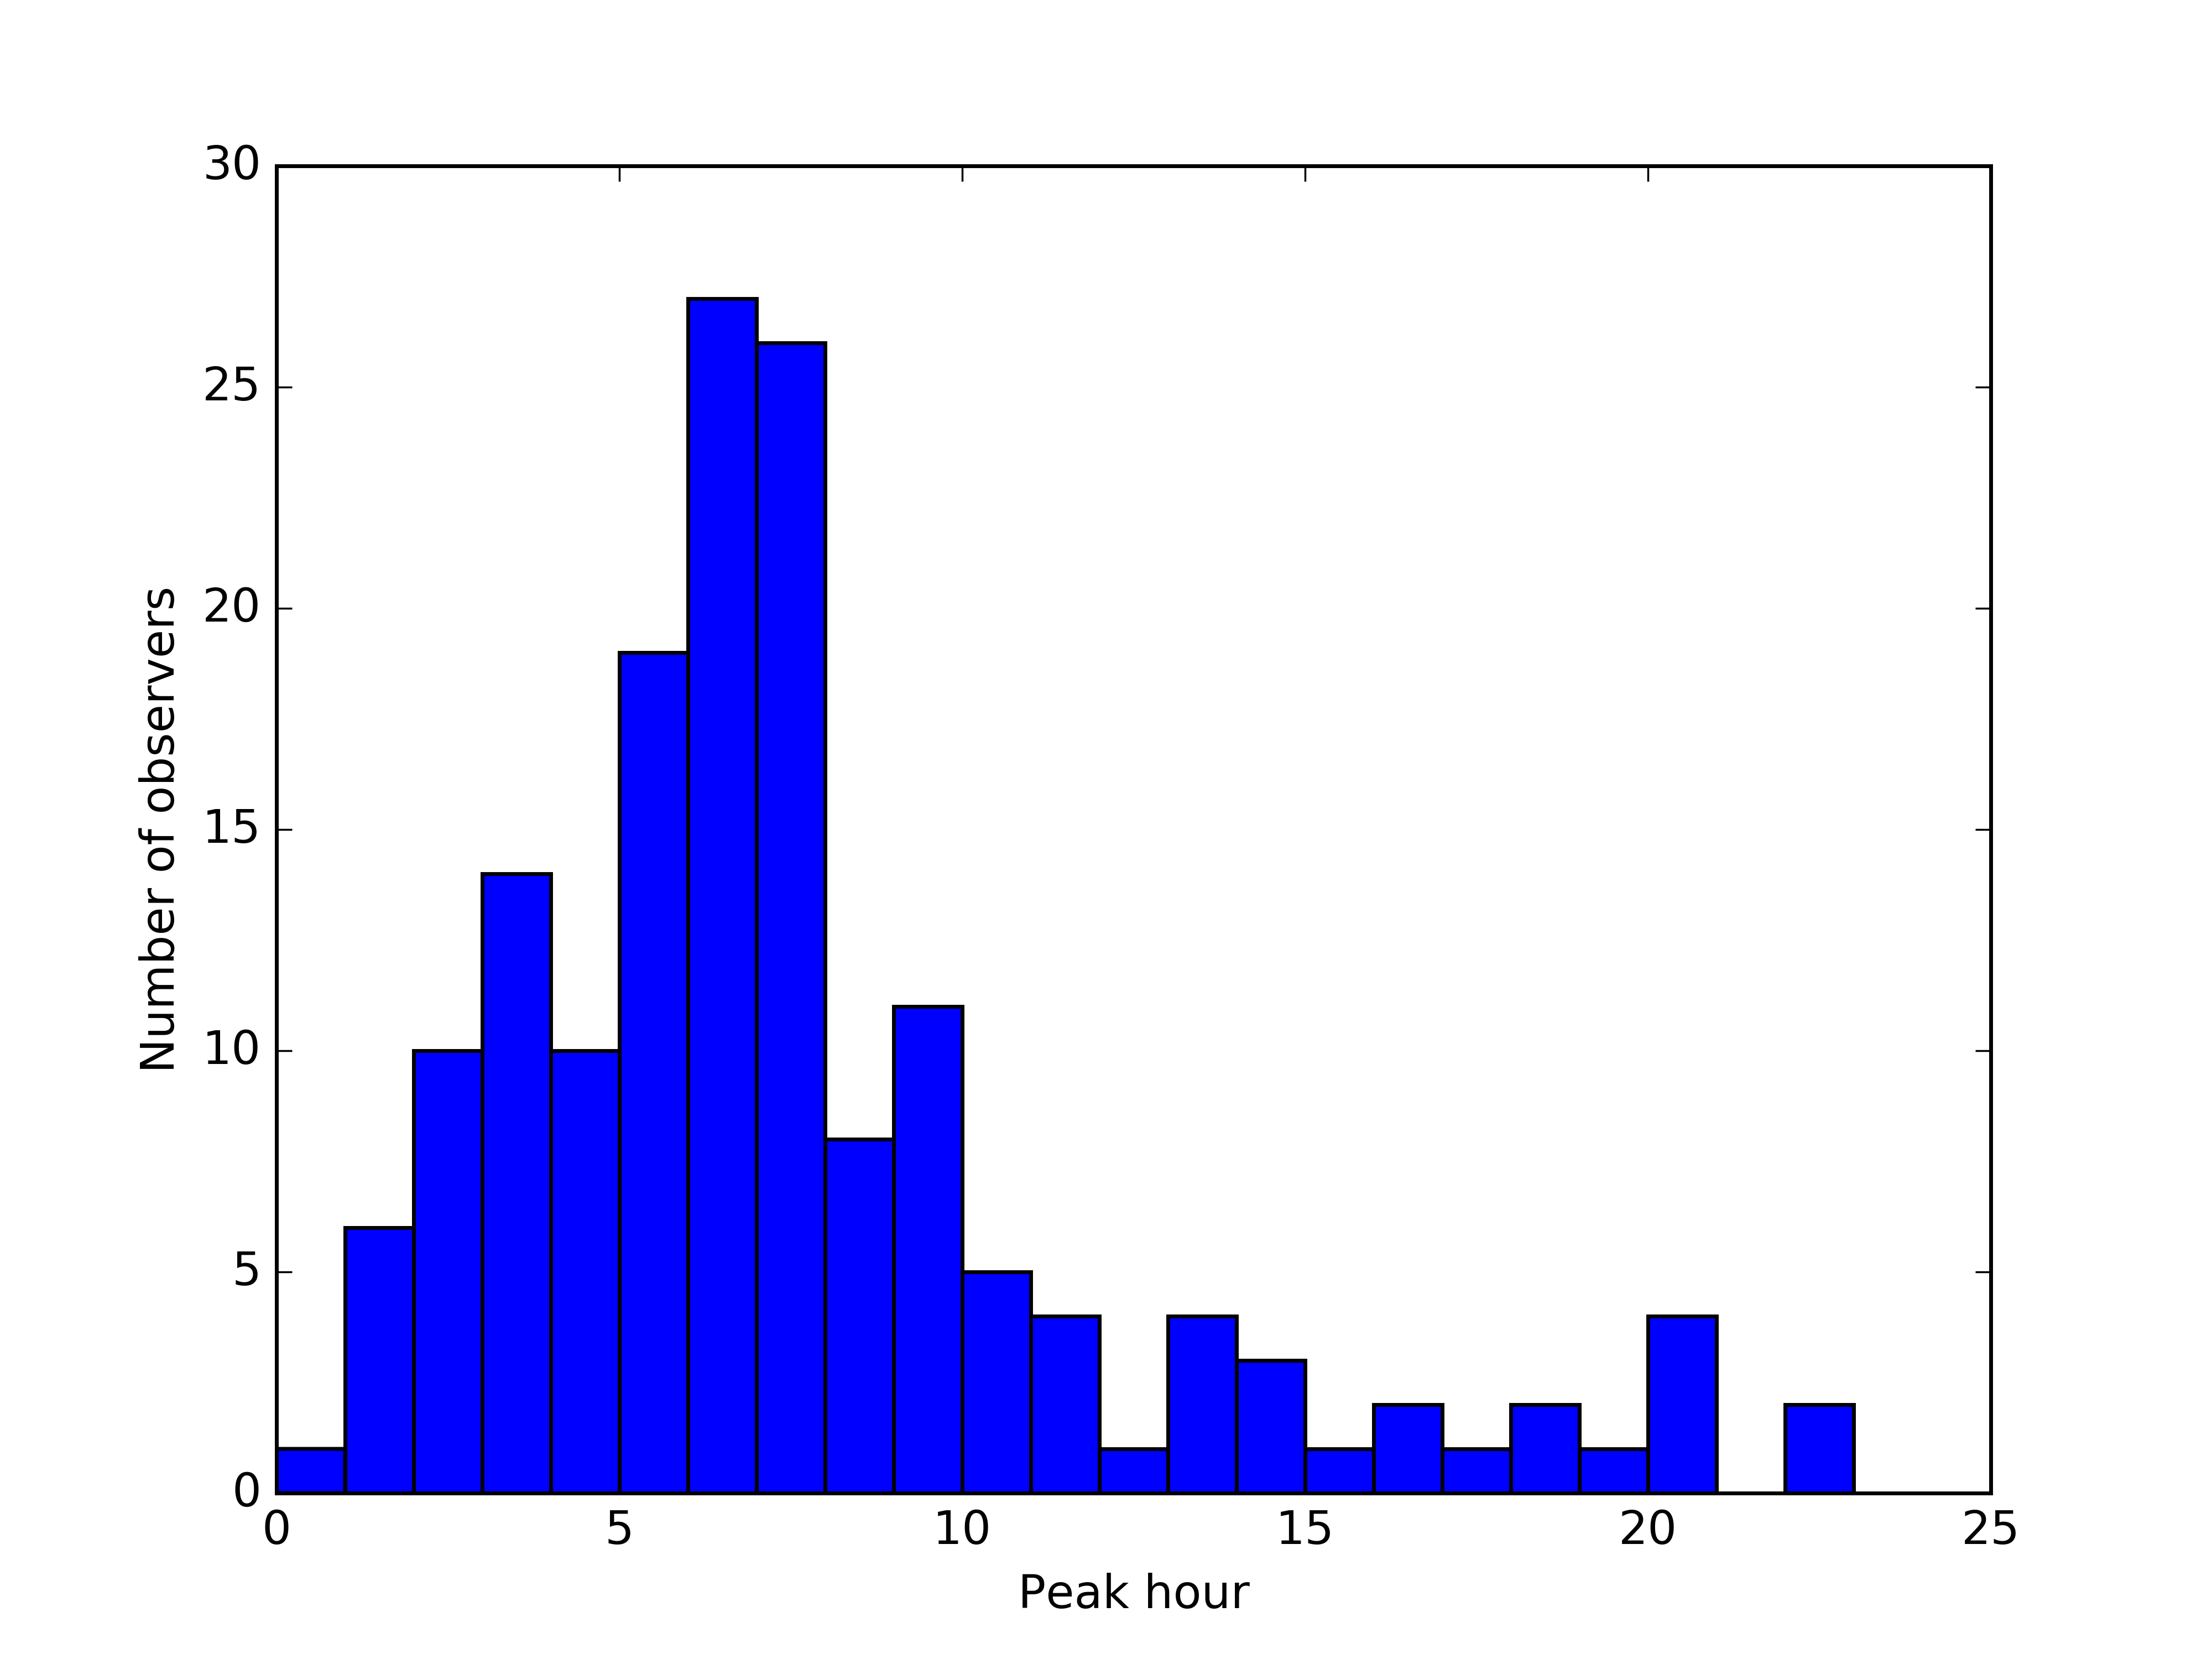
\includegraphics[width=\linewidth]{spatial/longitude/hist}
	\caption{Histogram of peak hours
		\label{fig:dishift:lon:hist}}
\end{figure}

The covariance varies a small amount with longitude other than a few categories. There does not appear to be a clear trend.  However, the poorest fits have large errors indicating that this is not a poor fit throughout observers in said categories. Consequently it would seem that the fit varies moderately across the globe. 
\begin{figure}[h!]
	\centering
	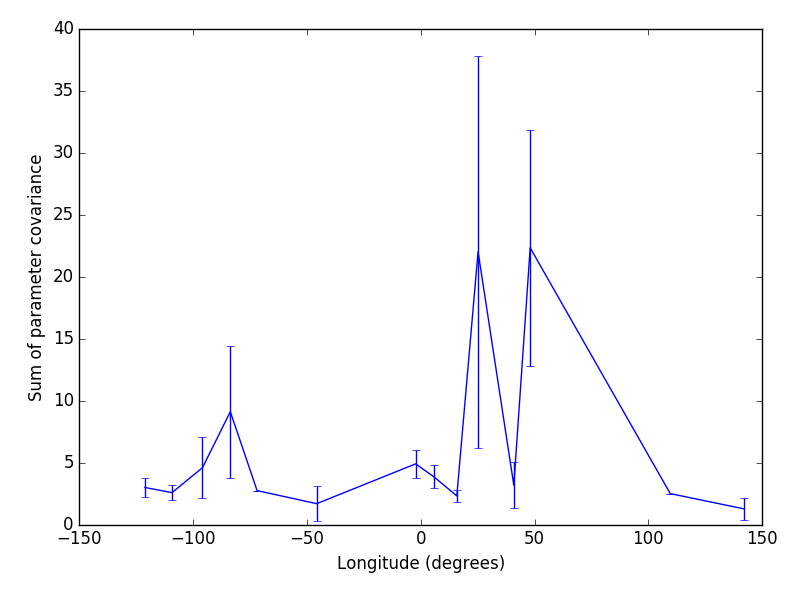
\includegraphics[width=\linewidth]{spatial/longitude/fit}
	\caption{Optimal sine function fit against longitude
		\label{fig:dishift:lon:fit}}
\end{figure}


\subsection{Temporal variation}
Figure~\ref{fig:dishift:temp:peak} shows the same result as previously noted. The variation for each location category varies around the hours expected if peak hour is correlated with longitude. There is a large amount of variation for the Asia \& Australia category, so it is hard to make an analysis from this. It is clear that in more recent years, there is less variation. Over time, no categories appear to increase or decrease, but instead fluctuate around certain values.
\begin{figure}[h!]
	\centering
	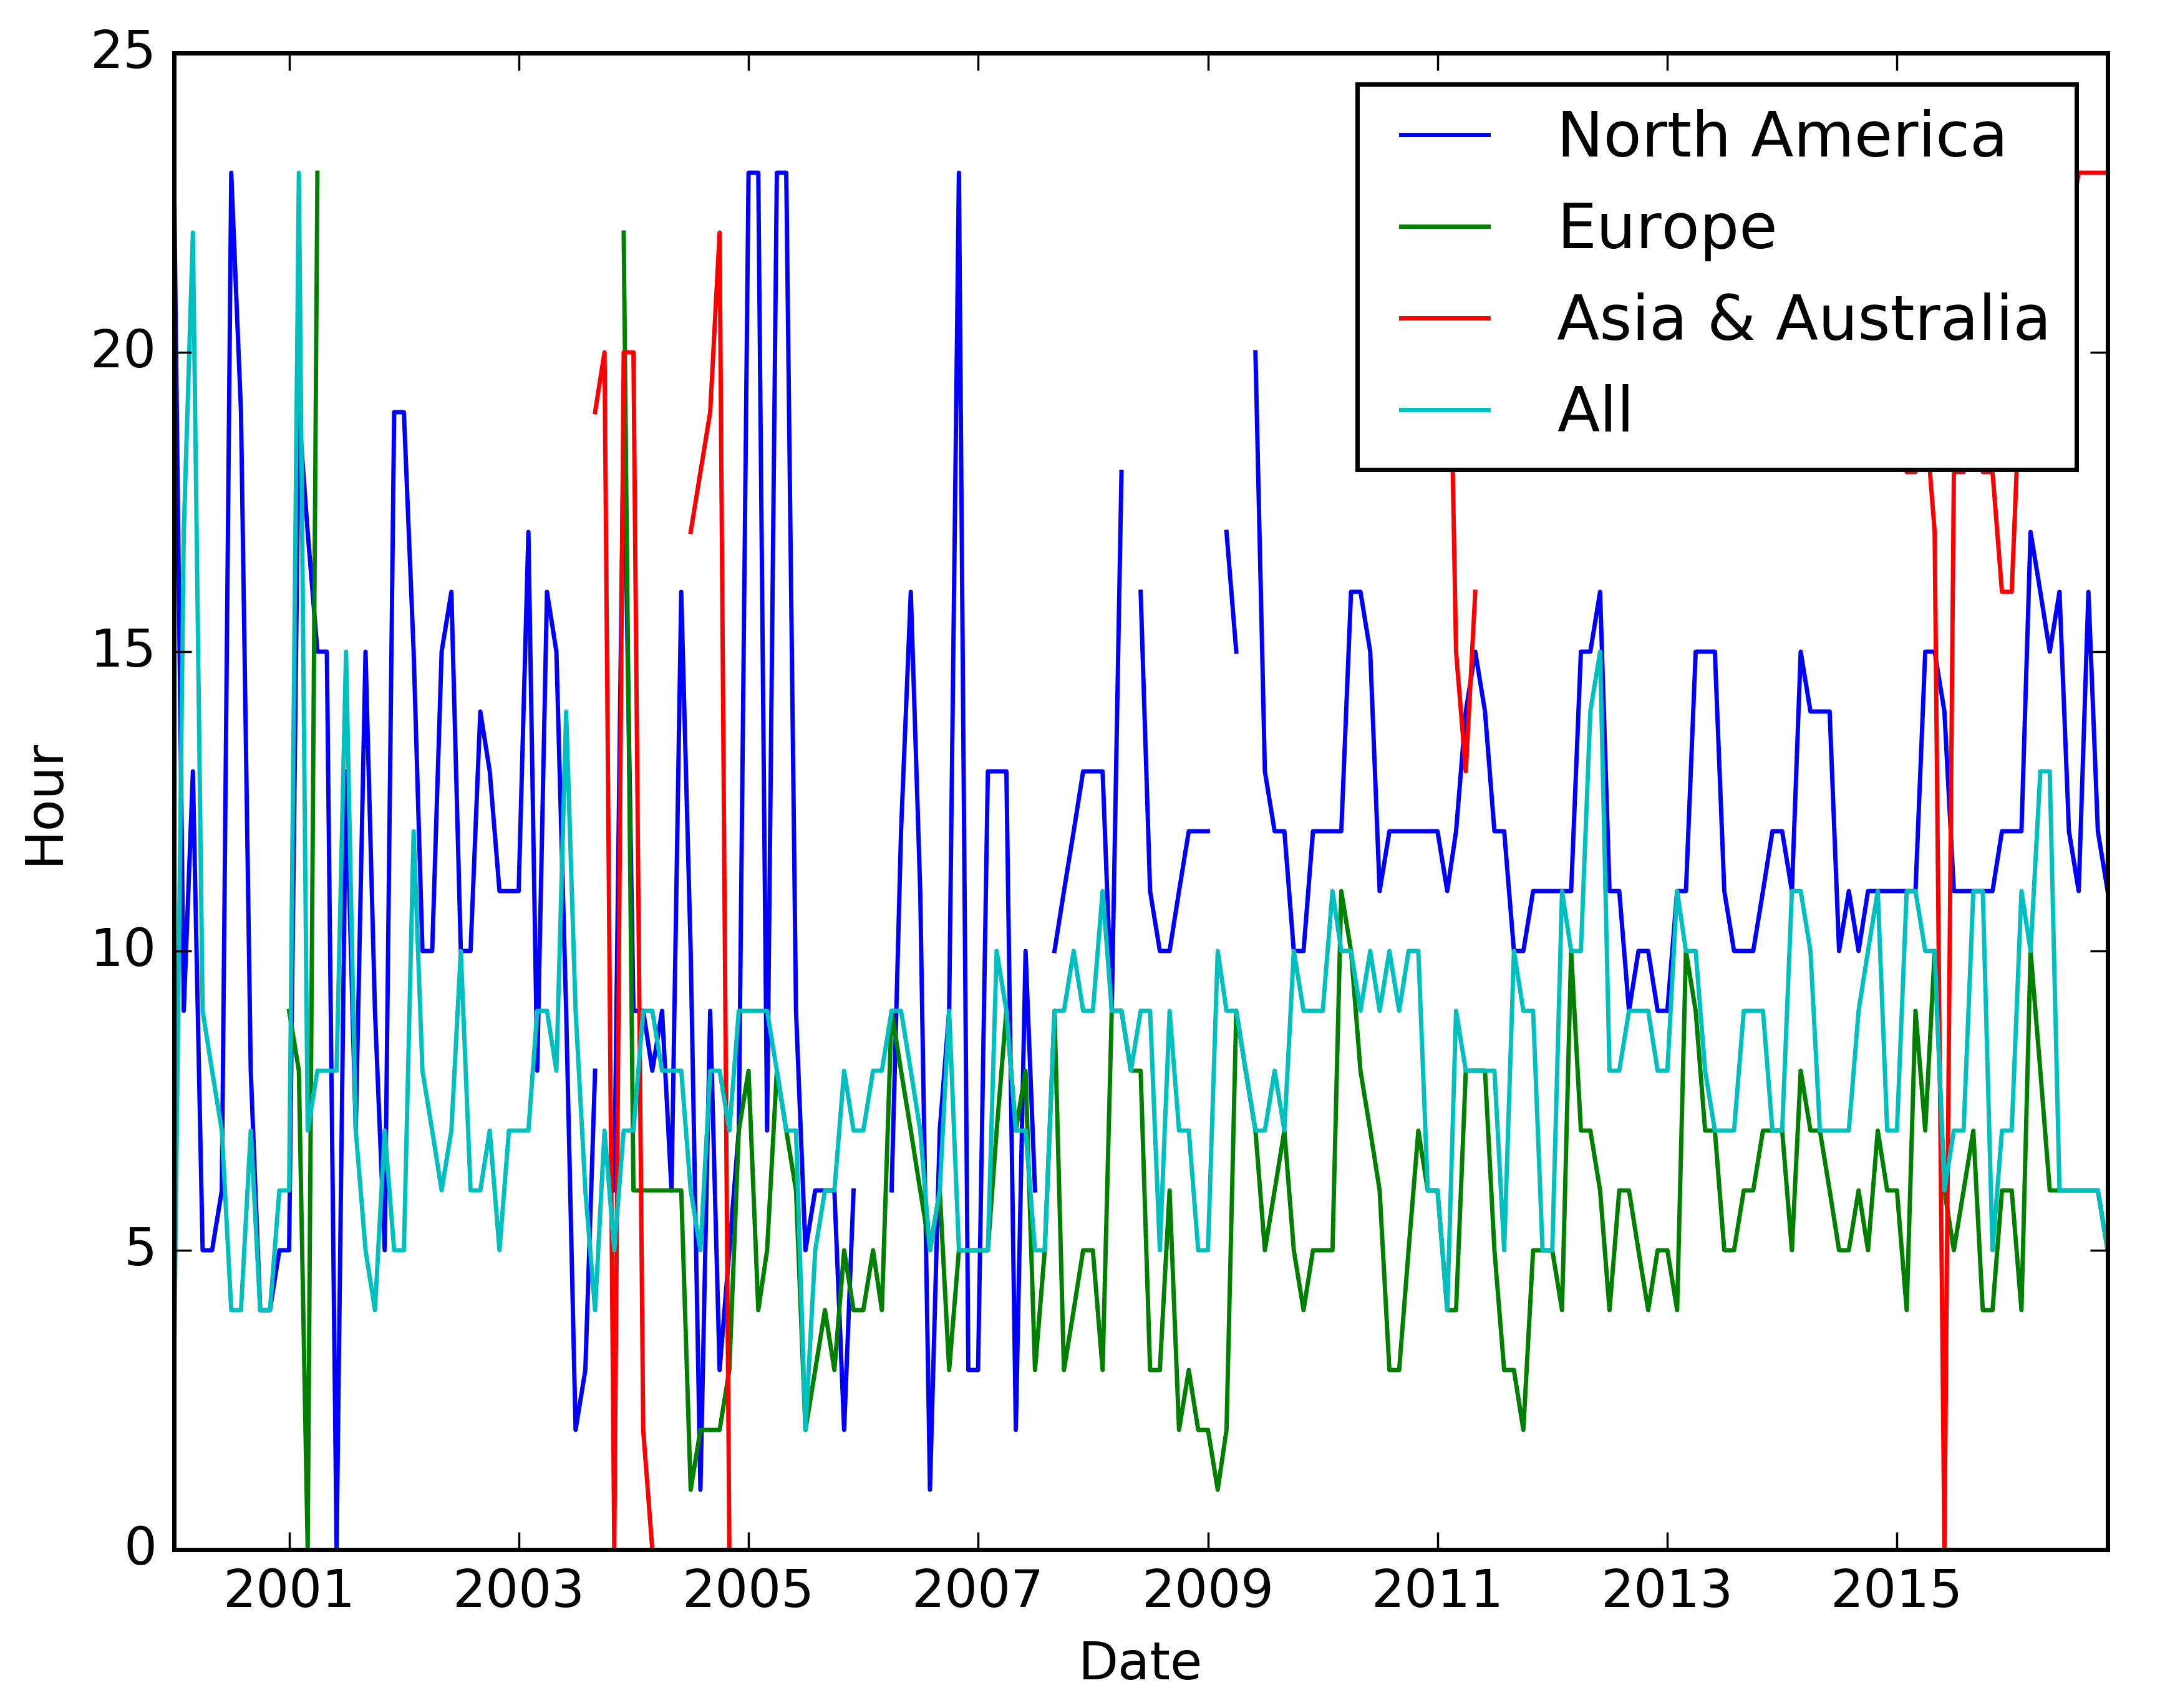
\includegraphics[width=\linewidth]{temporal/analyses/COMBINEDpeak}
	\caption{Peak hour of diurnal shift change over time
		\label{fig:dishift:temp:peak}}
\end{figure}
Generally, the fit is reasonably good. Between 2005 and 2011, the fits are much worse, indicating either a weaker diurnal shift (an unlikely phenomenon) or a more intense background level. For periods outside this, there is a low value of variation. All categories have a similar fit and absent trend over time.
\begin{figure}[h!]
	\centering
	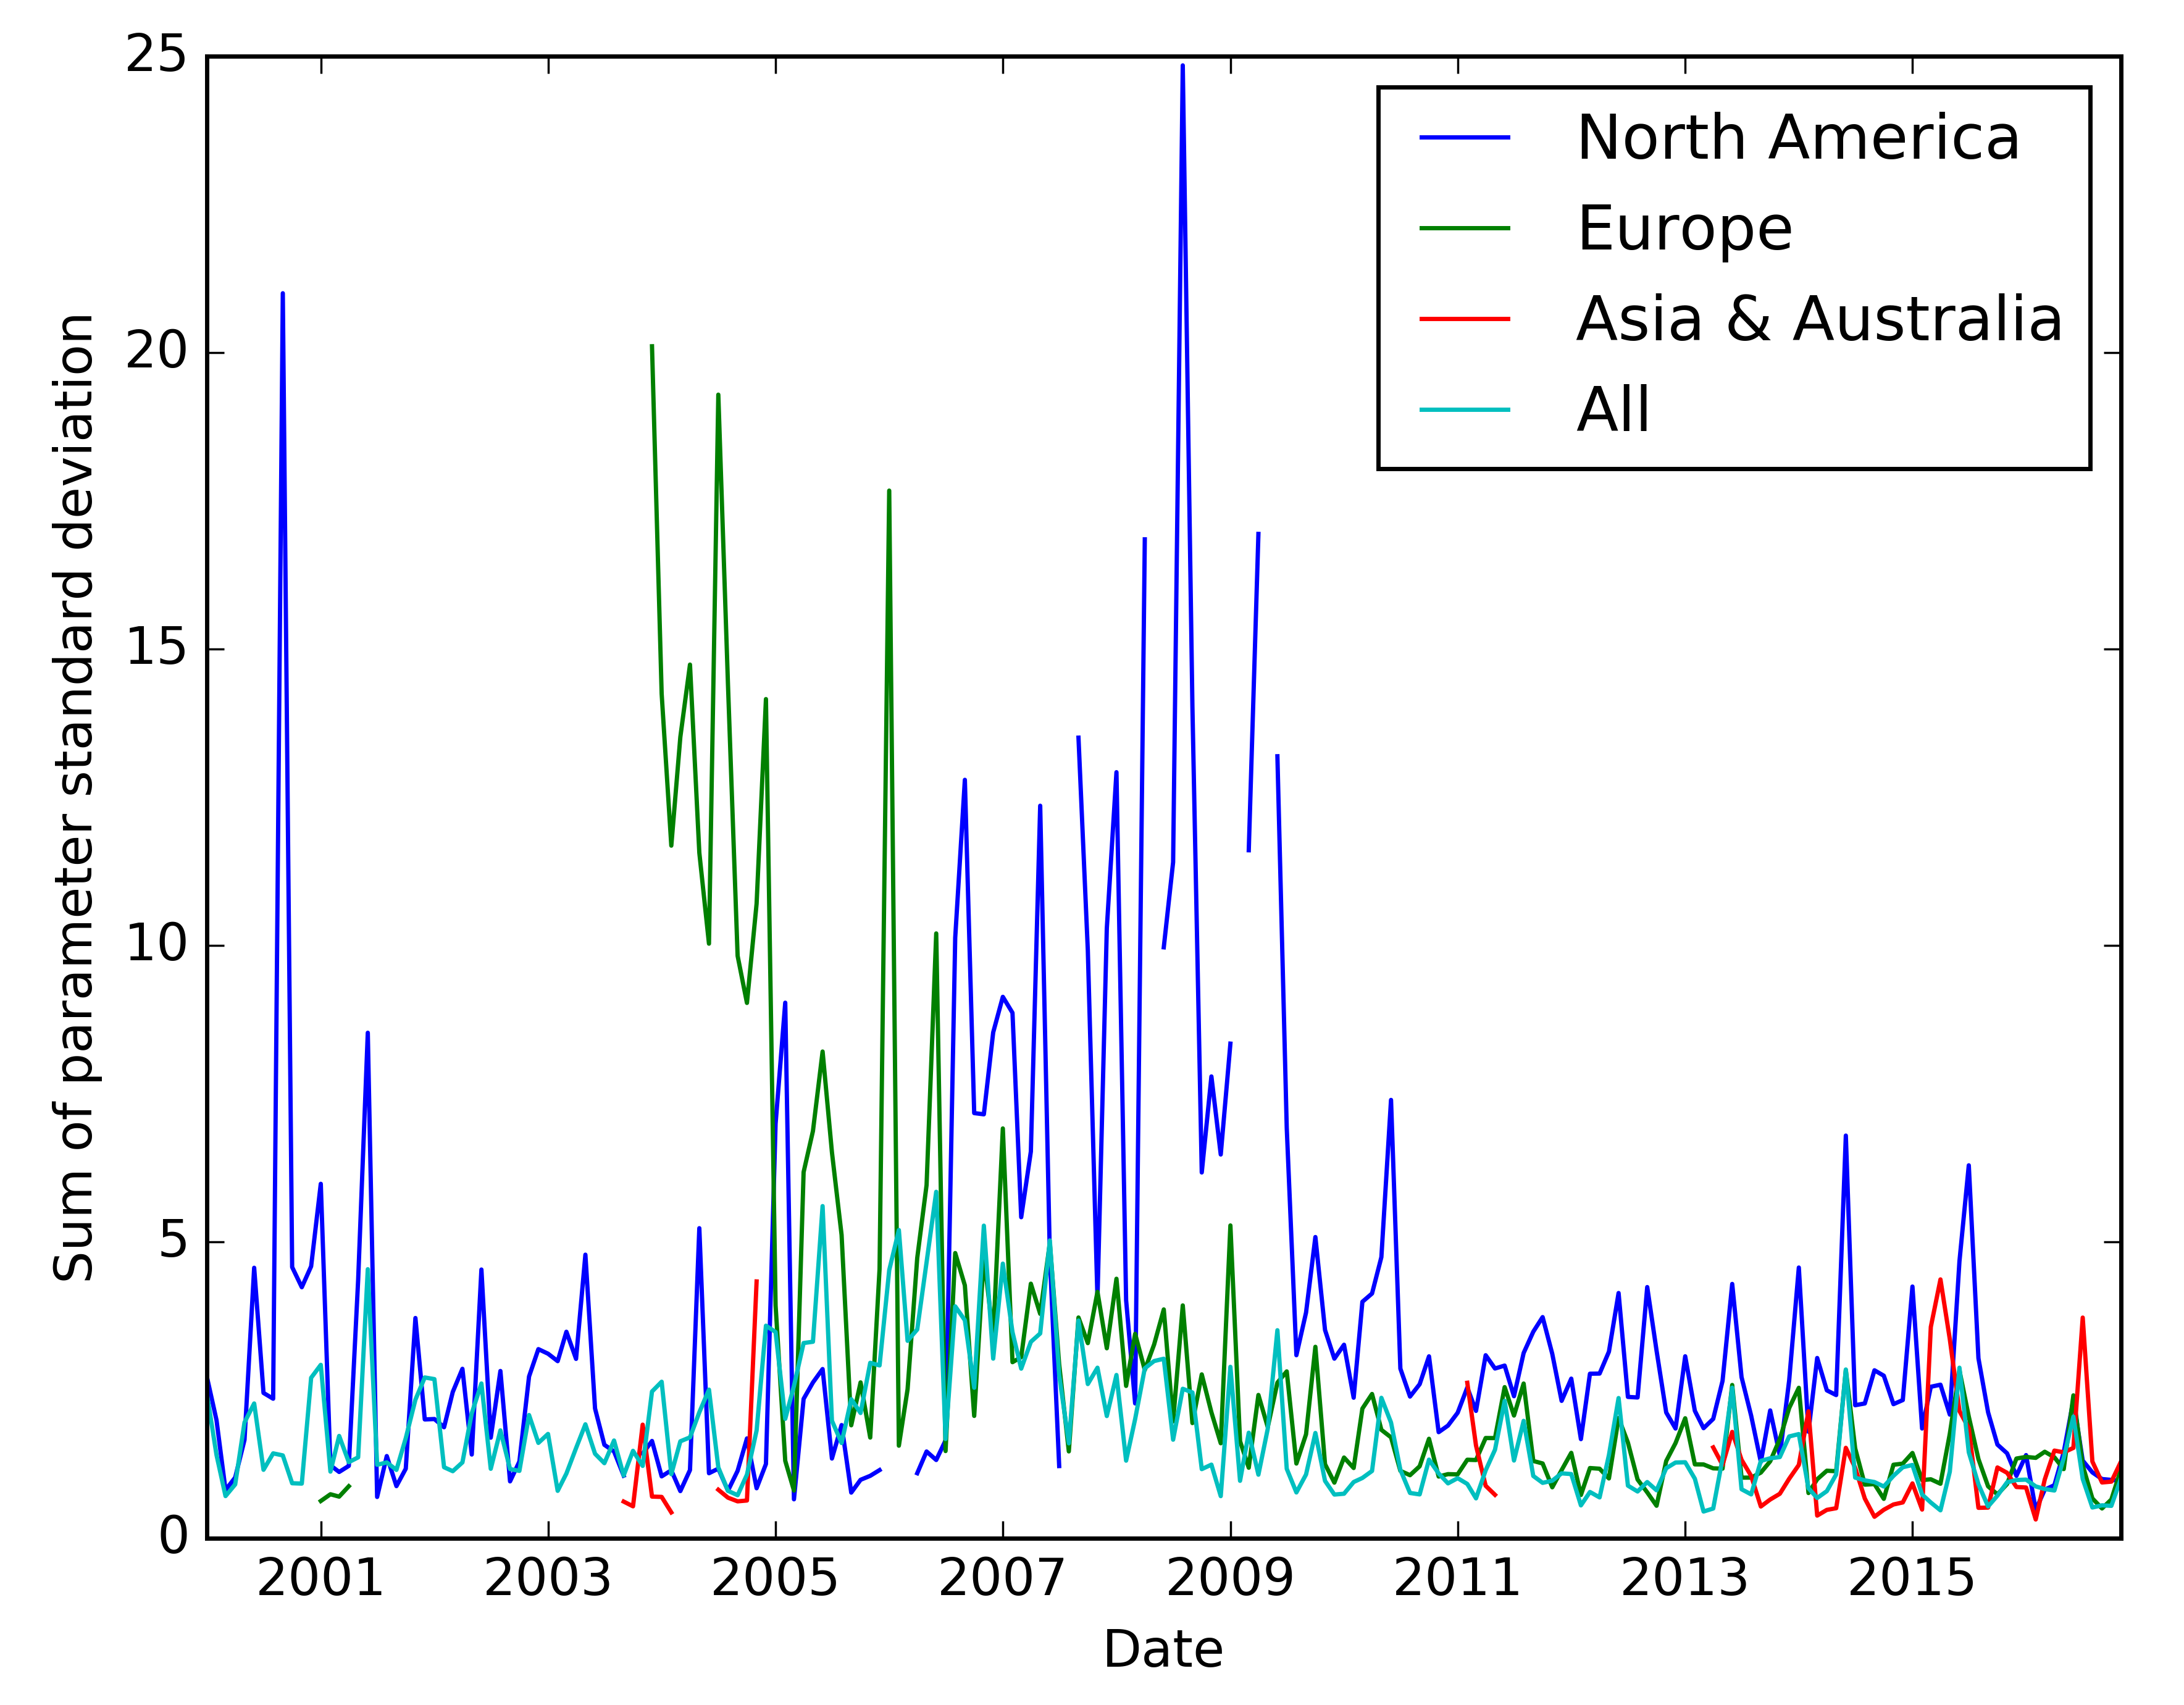
\includegraphics[width=\linewidth]{temporal/analyses/COMBINEDfit}
	\caption{Optimal sine function fit change over time
		\label{fig:dishift:temp:fit}}
\end{figure}
\subsection{Improvements}
\paragraph{Annual variation\\}
A question, that may reveal more information on the processes behind diurnal shift, is whether the phenomenon changes on a yearly time scale. Seasonal variation of diurnal shift may indicate an influence from sources such as the Sun, or the orientation of the Earth relative to it's orbit.
\paragraph{Intensity variation with latitude\\}
Singer, W., von Zahn, U., Batista, P. P., Fuller, B., \& Latteck, R. \cite{latitudes} analyse a variation of diurnal shift amplitude with latitude. Their analysis is over a relatively small range of latitudes. A further investigation, with a wider range of latitudes and more observers involved, could confirm or support their analysis. My own analysis indicates that there is little correlation.
\paragraph{Receiving station vs. detection station}
Most meteor detection setups are simply receiving stations. Typically a station, often a considerable distance away, emits a signal that reflects off of the meteor's ionised trail and is received by the observers, whose data are under consideration. This means that there is a difference between the longitude of the observer and the longitude of where the detection takes place. This will, of course, influence the conclusions made. Were the longitude of each detection station known, it may further support the conclusions of my model.
\section{Conclusion}
There is a clear correlation between longitude and peak hour of diurnal shift, as suggested by the model I propose. This is apparent from several results, including a histogram of peak hours. This good agreement indicates that my model is valid and is supported by the data. In addition, based on this analysis and previous analyses, it seems that there is little correlation between location and a sine function fit, suggesting that the intensity of diurnal shift (in the sense of relative intensity compared to background rates) is roughly uniform across the globe. However, there is no clear link to be made between the amplitude of diurnal shift and latitude. There appears to be a correlation, in general, with location, with a clear difference in amplitude between different location categories.
\chapter{Spacial variation of data characteristics}
\label{chap:spatial}
\begin{strip}
	\begin{minipage}{\textwidth}
		\begin{abstract}
			In the following chapter I present an analysis of variation of data characteristics by latitude and longitude. I find little correlation between data characteristics and latitude, and a limited correlation with longitude. However, I find supporting results for a model of diurnal shift. A symmetric distribution for meteor counts is suggested from the results.
		\end{abstract}
		\keywords{meteors, radio meteor detection, spacial variation, distribution}
	\end{minipage}
\end{strip}
\section{Background}
\textcolor{red}{Once chapter~\ref{chap:diurnalshift} is done, mention it in detail here}
The significance of this analysis includes a supporting argument for diurnal shift (see chapter~\ref{chap:diurnalshift}), and potential identification of locations with particularly good detection counts, which has implications for the levels of radio noise where the detection takes place. An analysis of detection rates based on both longitude and latitude could yield results that beg an investigation: perhaps at higher latitudes there are more meteors travelling tangential to the atmosphere, giving more detections?
\section{Literature Review}
\textcolor{red}{I can't seem to find any. What do?}
\section{Methodology}
In this chapter I present two analyses on the variation of certain data characteristics by latitude and longitude. In order to carry out these analyses, the observers from the RMOB data must be split into categories based on location.
\paragraph{Selecting observers\\}
Observers were selected based simply on whether they had Google Maps (GMAP) co-ordinates available. These co-ordinates are entered when uploading data to RMOB and are stored as part of the observer class location attributes dictionary. Provided an observer had {\it both} latitude and longitude available, then the analysis would be carried out on this data. Once all the observers had been checked and analysed (if necessary), the categorisation into groups could take place.
I used a basic process to group the observers, based on the difference between the current observer and the previous. Of course, the observers had to be sorted by increasing latitude or longitude (depending on the analysis) first. If the difference between co-ordinates was less than 10 degrees, then the two observers are considered part of the same group. This resulted in 9 categories for latitude, and 14 for longitude. These categories are not uniformly spread around the globe, but do provide a grouping of observers.
\paragraph{Analysis\\}
These characteristics summarise the data, namely 6 values: mean hourly count, max hourly count, skewness, peak hour of diurnal shift, fit to a sine function, and standard error. The standard error of all data for the observer is significant since it indicates how much the data varies over the time frame under consideration. A lower value indicates that the same detection count is generally seen, and a larger value indicates that the detection count varies erratically. The skew also indicates the distribution of the detection counts. A positive skew indicates that the detection counts trail off towards high values, whilst a negative skew indicates that the distribution is `steeper' for higher values, suggesting that there is a limit to the detection counts. The last two values are the peak hour of the diurnal shift, and the fit to an optimised sine curve for the mean detection counts over each hour of a day. This is calculated by averaging the values for all data for a given hour after midnight. A sine curve is in then fit to this, in the same process as chapter~\ref{chap:diurnalshift}, giving a sine function of the form $N = A \sin \left( \omega t + \phi \right) + \mu$ where $N$ is the detection count. The calculated `fit' is the sum of the covariances for $A$, $\mu$, and $\phi$. $\omega$ is assumed to be $\frac{2\pi}{24}$ so that the shift has a period of one day.
These 6 values will be calculated for each `entry' (month) for each observer, and then a mean will be taken from all the results for a given location category.

\section{Results}

\subsection{Latitude analysis}
\paragraph{Sample sizes \\}
Table~\ref{tab:spat:lat} shows the sample sizes for each latitude category.
\begin{table}[h!]
	\centering
	\begin{tabular}{ccc}
		\hline 
		Category & Latitude range ($^{\circ}$) & N$^o$ observers \\ 
		\hline 
		I & -43 -- -33 & 2 \\
		II & -31 -- -22 & 3 \\
		III & -20 -- -19 & 1 \\
		IV & -4 -- 5 & 3 \\
		V & 8 -- 12 & 2 \\
		VI & 23 -- 33 & 5 \\
		VII & 33 -- 44 & 33 \\
		VIII & 44 -- 53 & 107\\
		IX & 54 -- 57 & 9 \\  
		\hline
	\end{tabular} 
	\caption{Sample sizes for latitude categories \label{tab:spat:lat}}
\end{table}

\paragraph{Mean hourly detection count\\}
As can be seen in figure~\ref{fig:spat:lat:mean}, overall, the detection count is $\sim$ 60. There is a very low sample size for the category around a latitude of 0, which explains the large standard error. There does not appear to be an overall trend, there are no exceedingly anomalous results and there is no clear pattern across the categories. The minimum mean hourly detection count is category II ($\sim -30^{\circ}$) and the maximum is ($\sim 0^{\circ}$).
\begin{figure}[h!]
	\centering
	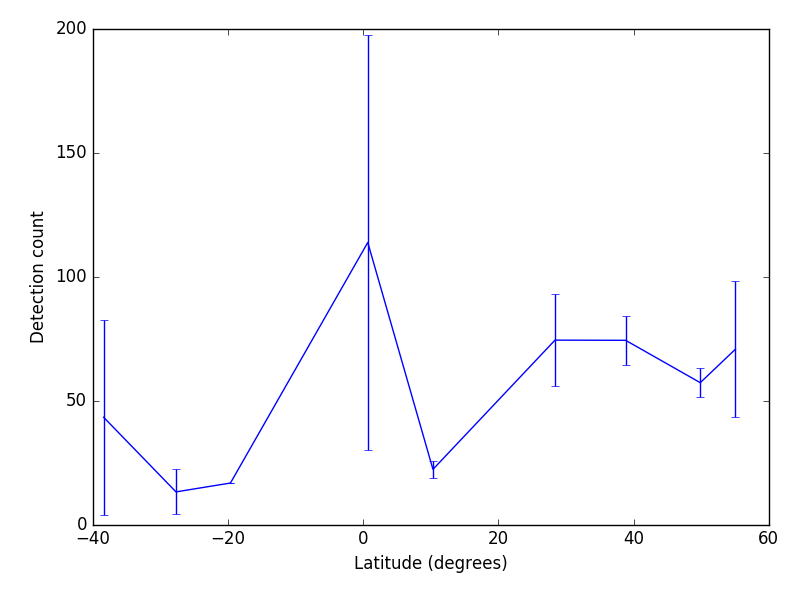
\includegraphics[width=\linewidth]{spatial/latitude/mean}
	\caption{Mean hourly detection count
		\label{fig:spat:lat:mean}}
\end{figure}
\paragraph{Maximum hourly detection count\\}
The standard errors are generally larger for the same categories compared to the mean hourly count. This suggests there is a much larger variation in the maximum count within each category. There is no clear trend over the latitude categories, as there is a large peak in category IV as well as VII. The lowest maximum hourly count is category III.
\begin{figure}[h!]
	\centering
	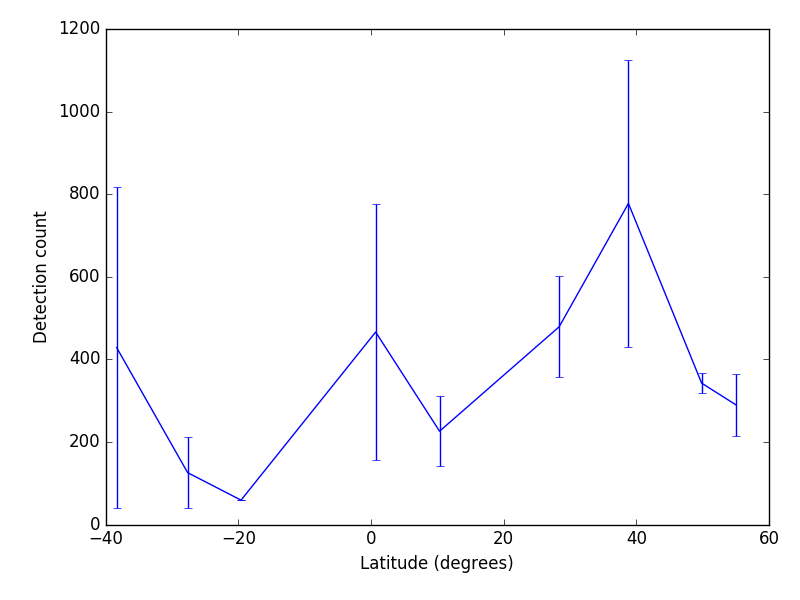
\includegraphics[width=\linewidth]{spatial/latitude/max}
	\caption{Maximum hourly detection count
		\label{fig:spat:lat:max}}
\end{figure}

\paragraph{Minimum hourly detection count\\}
For categories I -- VI the minimum is 1. This is as expected. Category IX has the largest minimum, though there is a large error, indicating the low sample size. Categories VII -- IX are the only categories without a minimum of 0. 
\begin{figure}[h!]
	\centering
	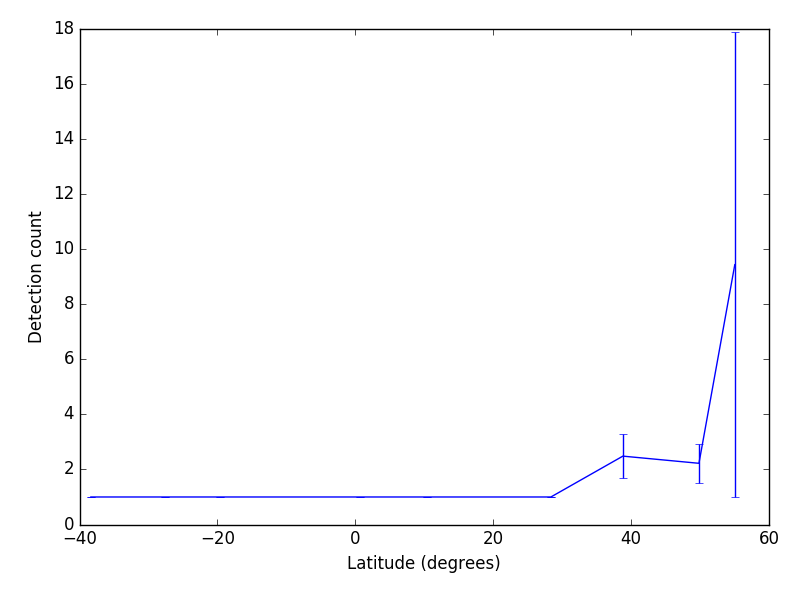
\includegraphics[width=\linewidth]{spatial/latitude/min}
	\caption{Minimum hourly detection count
		\label{fig:spat:lat:min}}
\end{figure}
\paragraph{Skewness\\}
Generally, the skewness is positive. There is a large error (relative to the values) indicating a widely varying skewness within each category. There is no clear trend, though the skewness {\it appears} to decrease as the latitude increases. There is only one category (V) with a negative skewness.
\begin{figure}[h!]
	\centering
	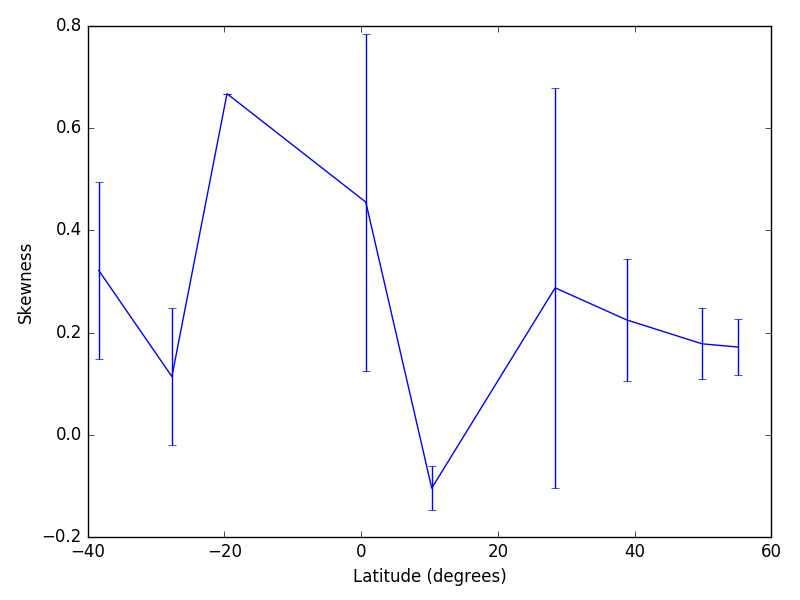
\includegraphics[width=\linewidth]{spatial/latitude/skew}
	\caption{Skewness of hourly counts
		\label{fig:spat:lat:skew}}
\end{figure}
\paragraph{Standard error\\}
The standard error appears to be relatively low for most of the categories, and with similar values, varying only by $\sim$ 3. The only exception to this is category IV, which has the largest standard error of $\sim$ 10, though there is a much larger error in this than the other categories. This could simply be an anomalous reading.
\begin{figure}[h!]
	\centering
	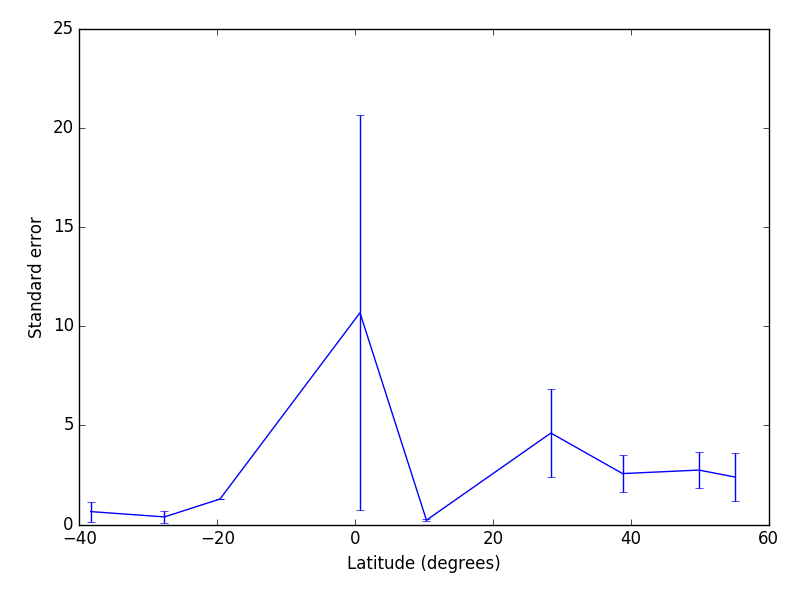
\includegraphics[width=\linewidth]{spatial/latitude/err}
	\caption{Variation in hourly detection count 
		\label{fig:spat:lat:err}}
\end{figure}
\paragraph{Diurnal shift\\}
There is no clear trend for the peak hour of the diurnal shift. There is a large error for most categories, for all categories at least an error of 1 hour. The large error indicates a large amount of variation within each category.
\begin{figure}[h!]
	\centering
	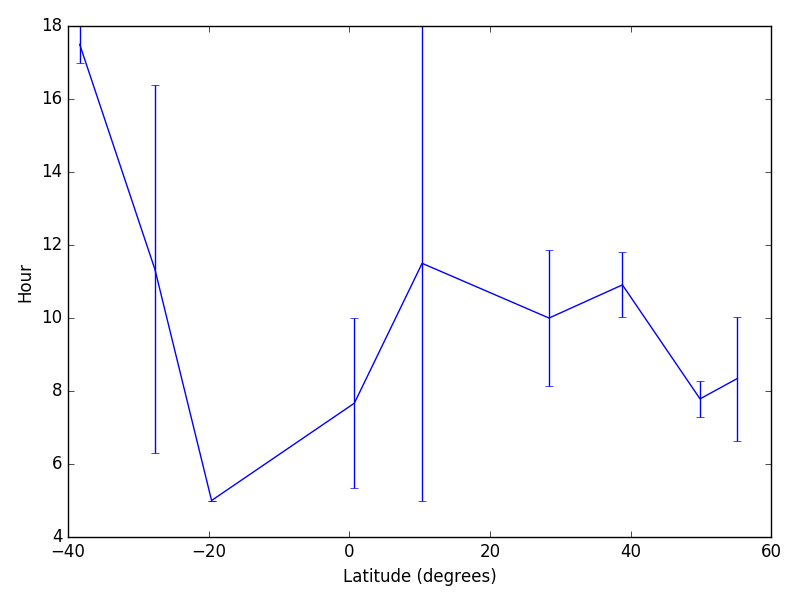
\includegraphics[width=\linewidth]{spatial/latitude/peak}
	\caption{Peak hour of diurnal shift
		\label{fig:spat:lat:peak}}
\end{figure}\\
For categories I--III and V, the fit is relatively good ($\sim$ 2). Categories VI -- IX have a slightly worse fit, around 6. Rather anomalously, category IV has a very poor fit, though in figure~\ref{fig:spat:lat:err} a large amount of variation is seen, so this is expected.
\begin{figure}[h!]
	\centering
	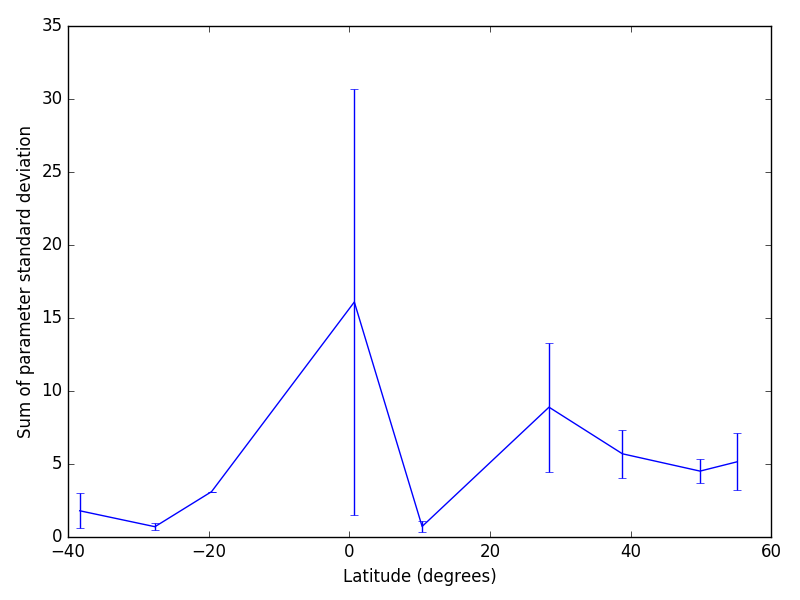
\includegraphics[width=\linewidth]{spatial/latitude/fit}
	\caption{Fit of diurnal shift to an optimal sine function
		\label{fig:spat:lat:fit}}
\end{figure}

\subsection{Longitude analysis}

\paragraph{Sample sizes\\}
Table~\ref{tab:spat:long} shows the sample sizes for each longitude category.
\begin{table}[h!]
	\centering
\begin{tabular}{ccc}
	\hline 
	Category & Longitude range ($^{\circ}$) & N$^o$ observers \\ 
	\hline 
	I & -123 -- -114 & 7 \\ 
	II & -112 -- -104 & 6 \\ 
	III & -100 -- -90 & 4 \\ 
	IV & -88 -- -78 & 4 \\ 
	V & -72 -- -71 & 1 \\ 
	VI & -48 -- -44 & 2 \\ 
	VII & -9 -- 0 & 56 \\ 
	VIII & 1 -- 12 & 32 \\ 
	IX & 12 -- 21 & 34 \\ 
	X & 22 -- 32 & 5 \\ 
	XI & 36 -- 46 & 4 \\ 
	XII & 47 -- 49 & 4 \\  
	XIII & 109 -- 110 & 1 \\ 
	XIV & 139 -- 148 & 3 \\  
	\hline
\end{tabular} 
\caption{Sample sizes for longitude categories \label{tab:spat:long}}
\end{table}

\paragraph{Mean hourly detection count\\}
There is no clear trend for the mean hourly count. The lowest mean is $\sim$ 10, for category VI. The maximum is XII, with a mean hourly count of more than 200. The errors are smallest for the categories with the largest sample sizes, namely categories VII -- IX.
\begin{figure}[h!]
	\centering
	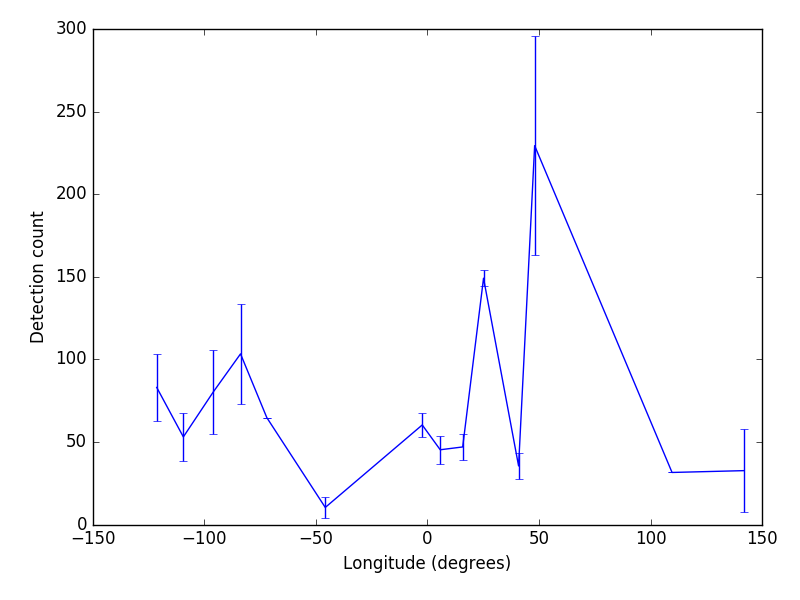
\includegraphics[width=\linewidth]{spatial/longitude/mean}
	\caption{Mean hourly detection count
		\label{fig:spat:lon:mean}}
\end{figure}
\paragraph{Maximum hourly detection count\\}
Most maximum hourly detection counts are around 500, though there is an anomalous maximum for category X, with a maximum of more than 4000. This is likely only a single observer, however, as indicated by the low sample size and large error.
\begin{figure}[h!]
	\centering
	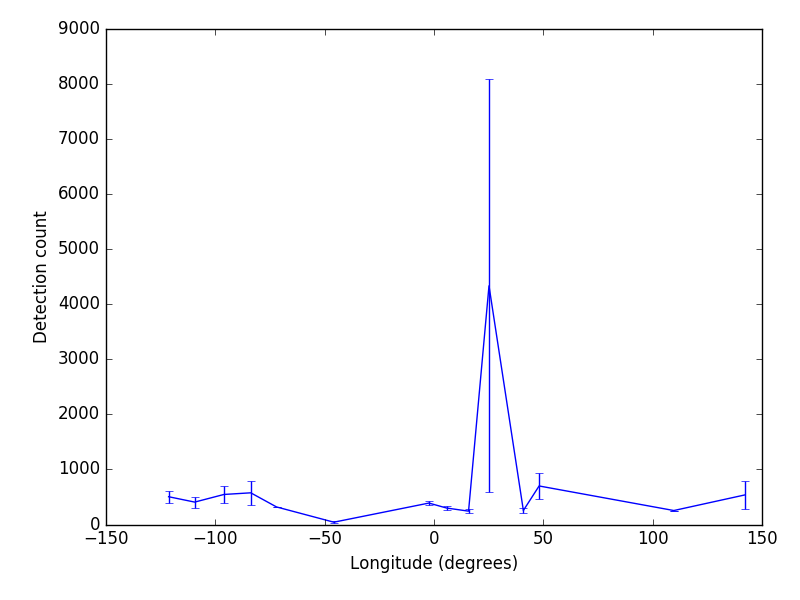
\includegraphics[width=\linewidth]{spatial/longitude/max}
	\caption{Maximum hourly detection count
		\label{fig:spat:lon:max}}
\end{figure}
\paragraph{Minimum hourly detection count\\}
The minimum values are, unlike in figure~\ref{fig:spat:lat:min}, not all 1. Most are a low value, though there is an anomalous result for XII, similar to the mean hourly count. This anomalous result is reflected by the large error.
\begin{figure}[h!]
	\centering
	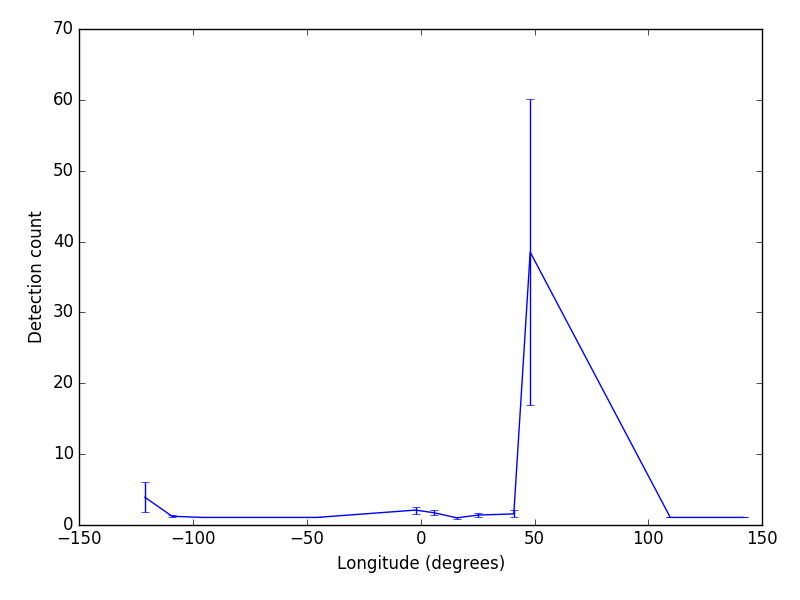
\includegraphics[width=\linewidth]{spatial/longitude/min}
	\caption{Minimum hourly detection count 
		\label{fig:spat:long:min}}
\end{figure}
\paragraph{Skewness\\}
9 out of 14 categories are positive. This is similar to figure~\ref{fig:spat:lat:skew}. There is a large error for most categories, indicating a large amount of variation within each category. This suggests there is little correlation between longitude and skewness of hourly counts.
\begin{figure}[h!]
	\centering
	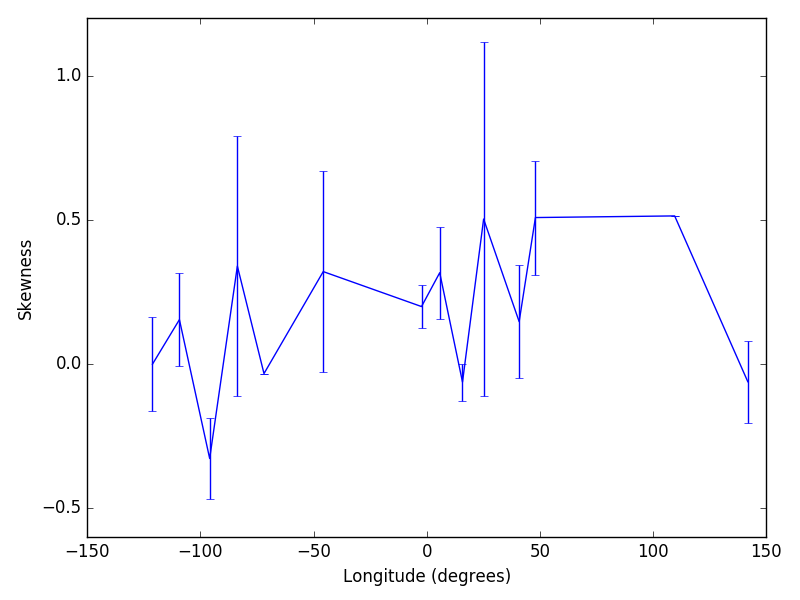
\includegraphics[width=\linewidth]{spatial/longitude/skew}
	\caption{Skewness of hourly counts
		\label{fig:spat:lon:skew}}
\end{figure}
\paragraph{Standard error\\}
Figure~\ref{fig:spat:lon:err} shows that there is a relatively low variation for most categories. The exceptions are categories X and XII, with errors of $\sim 10$ and $\sim 15$ respectively. There is a small error for all other categories, indicating a similar level of variation within the category.
\begin{figure}[h!]
	\centering
	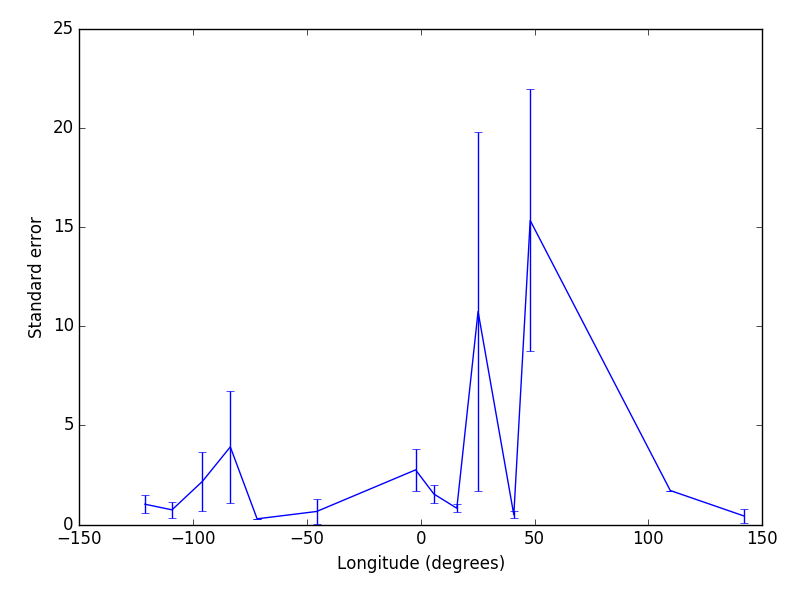
\includegraphics[width=\linewidth]{spatial/longitude/err}
	\caption{Variation in hourly detection count
		\label{fig:spat:lon:err}}
\end{figure}
\paragraph{Diurnal shift\\}
There appears to be a correlation between longitude and the peak hour of diurnal shift. This is discussed in more detail in chapter~\ref{chap:diurnalshift}. The peak hour is lowest for low longitudes, around 6, and larger for large latitudes, approximately 14 for a longitude of -125$^{\circ}$ and 125$^{\circ}$.
\begin{figure}[h!]
	\centering
	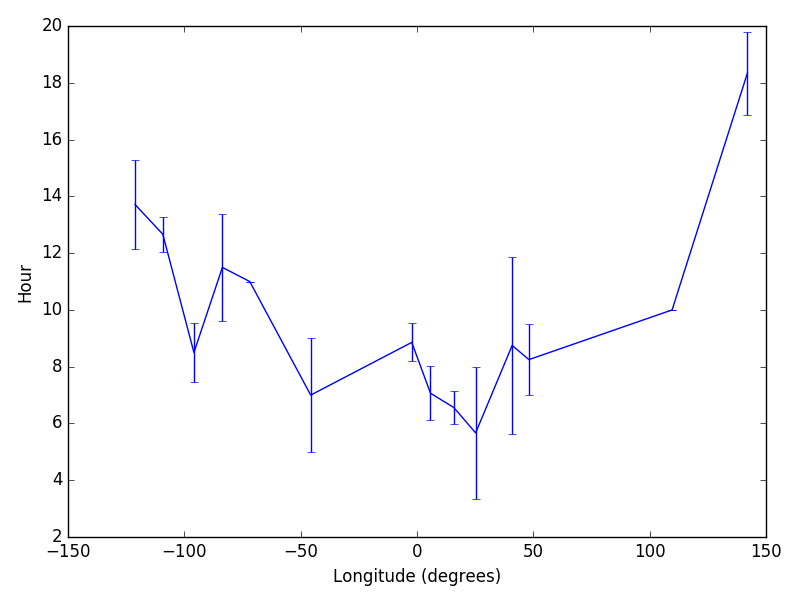
\includegraphics[width=\linewidth]{spatial/longitude/peak}
	\caption{Peak hour of diurnal shift
		\label{fig:spat:lon:peak}}
\end{figure}\\
Generally, the fit is around $\sim 4$ for all categories other than IV, X, and XII. There are very poor fits for categories X and XII, though these categories have anomalous readings in other analyses too. Other than these two categories, the errors are small.
\begin{figure}[h!]
	\centering
	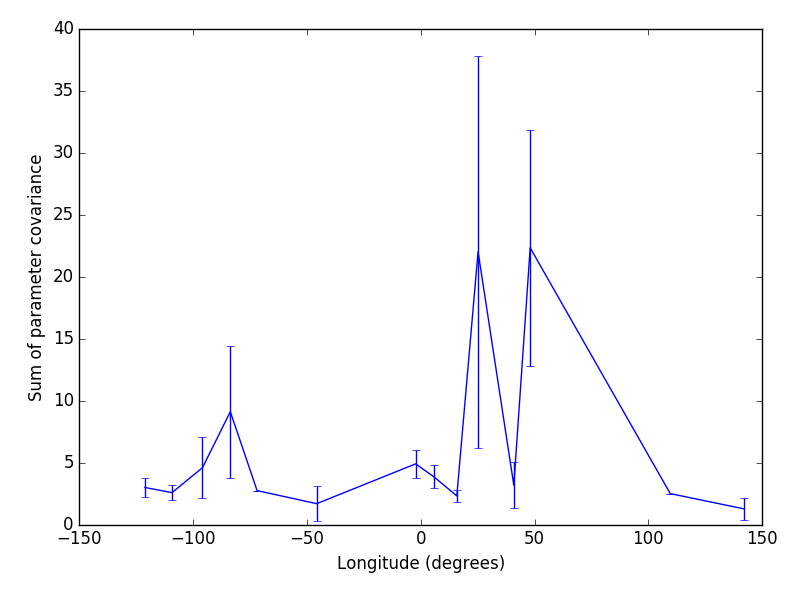
\includegraphics[width=\linewidth]{spatial/longitude/fit}
	\caption{Fit of diurnal shift to an optimal sine function
		\label{fig:spat:lon:fit}}
\end{figure}

\section{Discussion}
\subsection{Latitude analysis}
\paragraph{Mean, maximum \& minimum hourly count\\}
The mean does not appear to correlate with the latitude, but this is expected. Though the aim of this analysis was to determine if there are especially good locations for meteor detection, the reality is that on average, most places will be of the same quality for meteor detection. \\
It is not necessarily expected that the minimum {\it isn't} 1, though the reason is likely that most observers in the category {\it do} have a minimum of 1, but a few observers don't, which changes the mean minimum. This is a reasonable explanation, since the only categories that don't have a mean minimum of 1 have the largest sample sizes.
Larger variations in maximum are expected. The maximum has no limit (theoretically) though the minimum cannot be below 0, so variation in minimum is limited but this is not the case for maximum hourly detection counts.
\paragraph{Skewness\\}
The positive skewness is expected. There is likely to be more positive skew than negative, so on average it will be positive. Though most values are positive, they are all close to 0. This suggests that the distribution of meteor counts is symmetric.
\paragraph{Standard error\\}
There appears to be, on average, a small amount of variation in hourly counts. This was not expected: often counts may vary widely across the course of a day, though the range over which the variation takes place is apparently small enough that the standard error is not large.
\paragraph{Diurnal shift\\}
Correlation between latitude and the peak hour of an observer's diurnal shift is not expected, and this is reflected in the results. There is no apparent reason why the diurnal shift would vary with latitude, as discussed in chapter~\ref{chap:diurnalshift}.
\subsection{Longitude analysis}
\paragraph{Mean, maximum \& minimum hourly count\\}
There is no expectation for a correlation between the mean and the longitude. There is a large variation in the results, though without an analysis of location based on latitude {\it and} longitude, there is no way of knowing if the increased mean hourly detection counts are a result of the location or an observer's detection system.
\paragraph{Skewness\\}
Similar to the latitude analysis of skew, there is less grouping around 0 than expected. However, a slightly positive skew is not anomalous: counts will trail off towards larger numbers, but will never be below 0, giving a slightly positive skew.
\paragraph{Standard error\\}
The large increase in standard error for categories X and XII are obscure. This increase could be due to the location, but most likely it is a result of the set up of the observers in the sample. This would explain the anomalous results, since the low sample sizes of 5 and 4 respectively would allow for a large variation due to a single observer's counts.
\paragraph{Diurnal shift\\}
The apparent correlation between longitude and peak hour of diurnal shift is discussed in detail in chapter~\ref{chap:diurnalshift}. It is an expected result based on the model for diurnal shift.
\subsection{Improvements}
\paragraph{Percentiles\\}
Analysing the maximum and minimum hourly detection counts can only reveal a certain amount of information. It does give {\it some} indication towards the distribution of hourly counts, but taking quartiles, or 90th and 10th percentiles, will give more indication. The maximum may be extremely large, but there are no other values similar to it for a given observer, in which case the 90th percentile would reveal a lot more about the distribution. Similarly, the minimum is likely to always be 0 or 1, which does not provide much information, whilst the 10th percentile would indicate how many hourly counts are this small.
\paragraph{Joint latitude \& longitude analysis\\}
Whilst analysing latitude and longitude individually reveals, or thwarts, correlations, it is not as valuable as a joint analysis. This could be represented using a 3D plot, and would indicate much more clearly hotspots for meteor detection, and may reveal correlations that are not solely between latitude and longitude, but a correlation between the two.

\section{Conclusion}
There does not appear to be a large degree of correlation between most data characteristics and latitude or longitude. There appears to be a correlation between peak hour of diurnal shift and longitude, as expected based on the models discussed in chapter~\ref{chap:diurnalshift}. There are clearly anomalous readings for some results, namely standard error (longitude) and minimum hourly detection count (latitude). Likely explanations for this are low sample sizes. Further work, focusing on longitude and latitude, may clarify some results, indicating which apparent trends persist and which are anomalous.
\chapter{Temporal Variation of Radar Counts \& Data Characteristics}
\label{chap:temporal}
\begin{strip}
	\begin{minipage}{\textwidth}
		\begin{abstract}
			I present a study of the variation through time of radio meteor detection counts and characteristics of observer data. Results indicate a significant increase in radar counts between 2005 and 2011. I expand on previous research by Lindblad \cite{lindblad} and Bumba \cite{bumba}, providing these results which support their hypotheses of correlation between radar counts and solar activity. I also find an increase in meteor counts towards the middle of the year and discount day-night variation as a cause of increased counts.
		\end{abstract}
	\end{minipage}
\end{strip}
\section{Overview}
In this chapter I investigate temporal variations in meteor detection count over time. There are many patterns that arise in meteor detection: diurnal shift over the course of a day, and showers causing variation over the course of a year. These variations can occur because of a variety of factors. In chapter~\ref{chap:diurnalshift} I have investigated the cause of diurnal shift, in chapter~\ref{chap:zhr} I have investigated meteor showers. In this chapter I will analyse the variation of counts on a diurnal, monthly and annual scale.\\
Knowledge of the variation seen in meteor detection may help to improve methods such as Zenithal Hourly Rate (ZHR); by providing a better understanding of the background detection counts, normalising data to investigate meteor showers can become easier. See chapter~\ref{chap:zhr} for more on ZHR. Of significance is a comparison between these results and other analyses of temporal variation, but for visual detection: will radio detection be more influenced? Are the same variations seen? This analysis will demonstrate whether any variation is a worldwide phenomenon since the data set includes observers from across the globe.
\section{Literature Review}
\label{sec:temp:litrev}
Lindblad (1968) \cite{lindblad} provides a similar analysis on long-term variation in meteor radar rates, as well as echo amplitudes. In this paper it is seen that the echo amplitudes correlate with the electron line density, indicating an influence from the solar wind. It is also observed that long-term variation in radio meteor detection count can be explained qualitatively by a variation in atmospheric density in the region where most meteors burn up, which itself is related to the solar cycle. During solar minimum, the shortest ionisation trails are seen, as well as higher electron line densities, suggesting that meteor echo signal strength will be greater at solar minimum.\\
Bumba (1948) \cite{bumba} calculated the yearly rate of meteors as a function of position in the solar cycle, demonstrating that there is an inverse relationship between solar activity and detection counts, that is, counts are maximised when solar activity is at a minimum.
\section{Methodology}
There are two main analyses. 
\subsection{Data characteristics}
The first is an analysis of the variation over time of characteristics that summarise the data, specifically 4 values. (Note that these are the same as chapter~\ref{chap:diurnalshift} and \ref{chap:spatial}, other than the mean, minimum and maximum values which are not included in this analysis). The standard error of all data for the observer is taken, which indicates how much the data varies. A lower value indicates that the same detection count is generally seen, and a larger value indicates that the detection count varies erratically. The skew also indicates the distribution of the detection counts. A positive skew indicates that the detection counts trail off towards high values, whilst a negative skew indicates that the distribution is `steeper' for higher values, suggesting that there is a limit to the detection counts. The last two values are the peak hour of the diurnal shift, and the fit to an optimised sine curve for the mean detection counts over each hour of a day. This is calculated by averaging the values for all data for a given hour after midnight. A sine curve is in then fit to this, in the same process as chapter~\ref{chap:diurnalshift}, giving a sine function of the form $N = A \sin \left( \omega t + \phi \right) + \mu$ where $N$ is the detection count. The calculated `fit' is the sum of the covariances for $A$, $\mu$, and $\phi$. $\omega$ is assumed to be $\frac{2\pi}{24}$ so that the shift has a period of one day. These 6 values will be calculated for each observer, then the mean is recorded for all data for each month of each year.
\subsection{Detection counts}
The second analysis is of the mean hourly detection counts for all observers in the sample, over various scales. The scales being considered are daily, monthly and yearly. For yearly the mean will be taken over the entire year, and also each month in a year, to give a higher resolution of the variation. A similar analysis, on the yearly scale, will be completed which uses data solely from the night-time, or day-time (for the location of the observer).
\subsection{Analysis by location}
For each of the above analyses, they will be repeated for data from all observers around the world from the RMOB data set, as well as specific locations, namely observers from Europe, Asia \& Australia, and North America. The sample sizes for observers in each location category are shown in table~\ref{tab:temp:sizes}.
\begin{table}
	\centering
	\begin{tabular}{cc}
		\hline
		Location & N$^o$ observers \\
		\hline 
		Europe & 220 \\
		North America & 37 \\
		Asia \& Australia & 12 \\
		\hline
	\end{tabular}
	\caption{Sample sizes for location categories 
		\label{tab:temp:sizes}}
\end{table}
\section{Results}
\subsection{Data characteristics}
\paragraph{Standard error\\
	\label{par:err}}
From figure~\ref{fig:temp:err} it is clear that the standard error is relatively small, and does not vary a great deal long term. There are short-term anomalies, for example in 2000 and 2008, for observers located in North America, and in 2005 for observers located in Europe. There is a clear increase in standard error for all categories from 2005 to 2011. The variation within each year does not appear to be periodic.
\begin{figure}[h!]
	\centering
	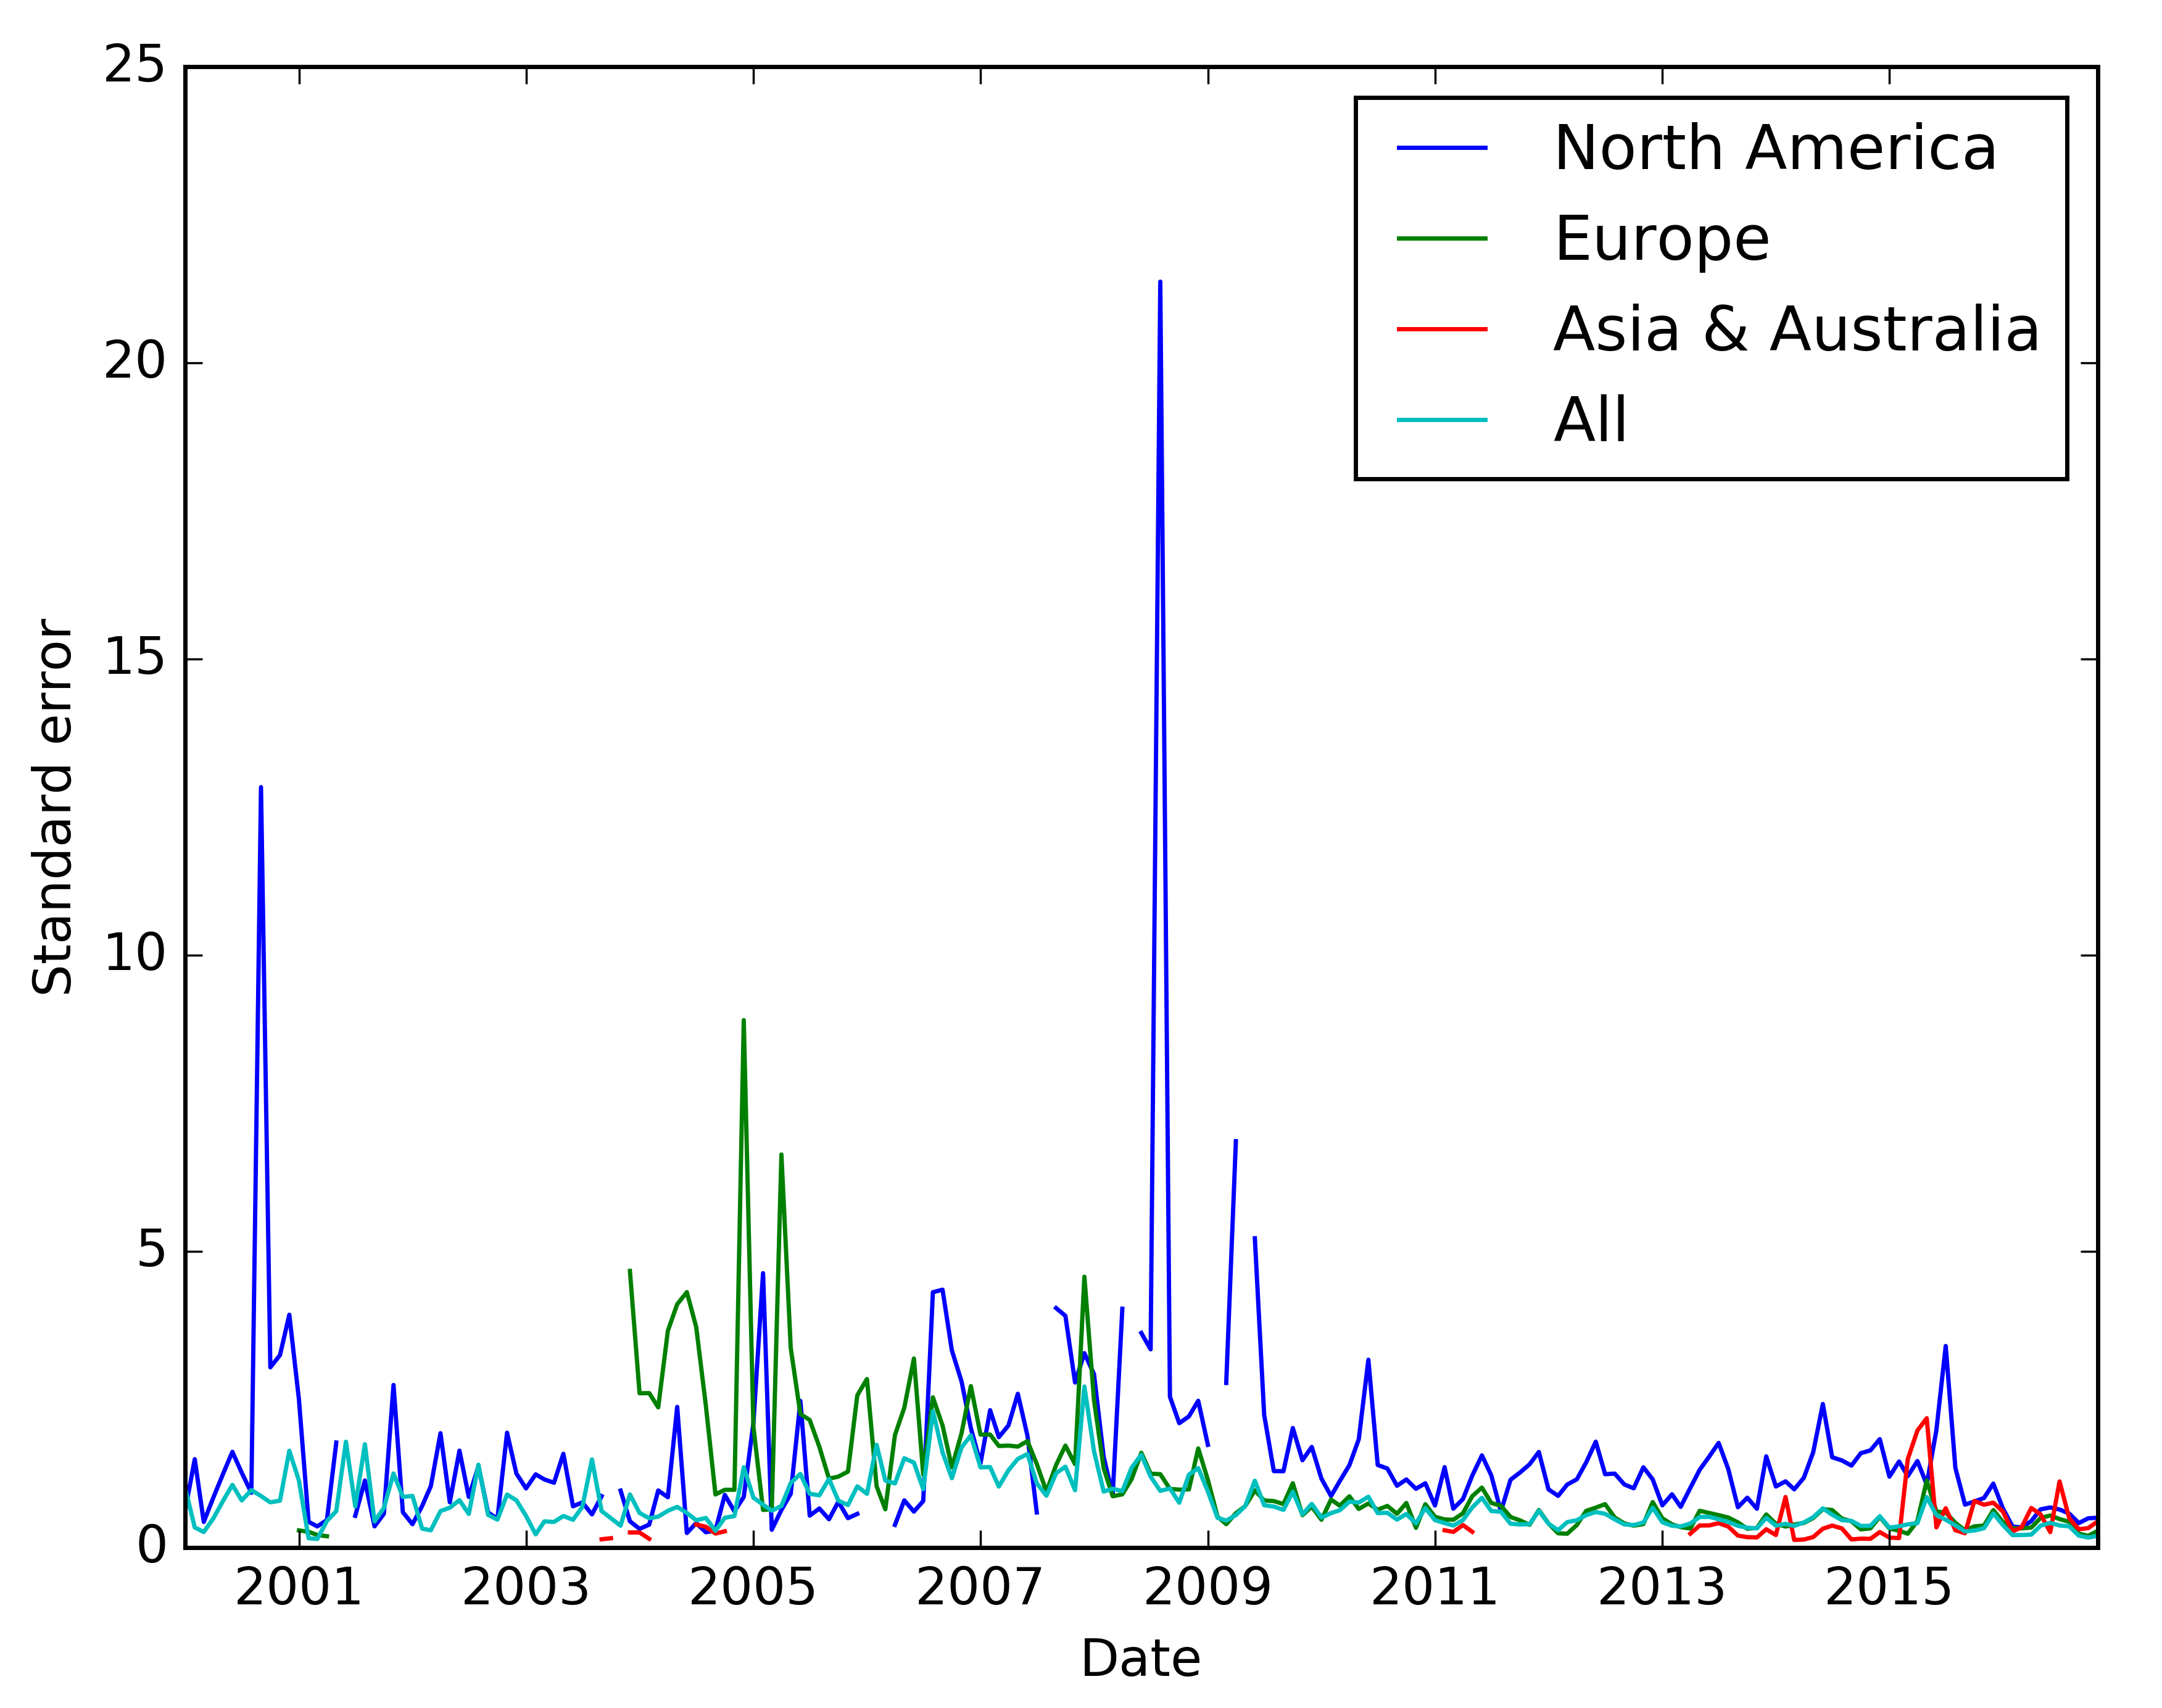
\includegraphics[width=\linewidth]{temporal/analyses/COMBINEDerr}
	\caption{Variation of standard error
		\label{fig:temp:err}}
\end{figure}
\paragraph{Skewness\\}
There does not appear to be a long term trend. The skewness is generally larger than 0, however it varies by $\sim$1, around 2000. This variation decreases over time, and the skewness appears to be closer to 0 for years 2005 onwards. There are anomalous results, but they are short term. For observers located in Europe, the skewness dips below 0 around 2005-2011 before fluctuating around 0 from 2011 onwards. This is the same for all categories; the values fluctuate around 0 between 2011 and 2015.
\begin{figure}[h!]
	\centering
	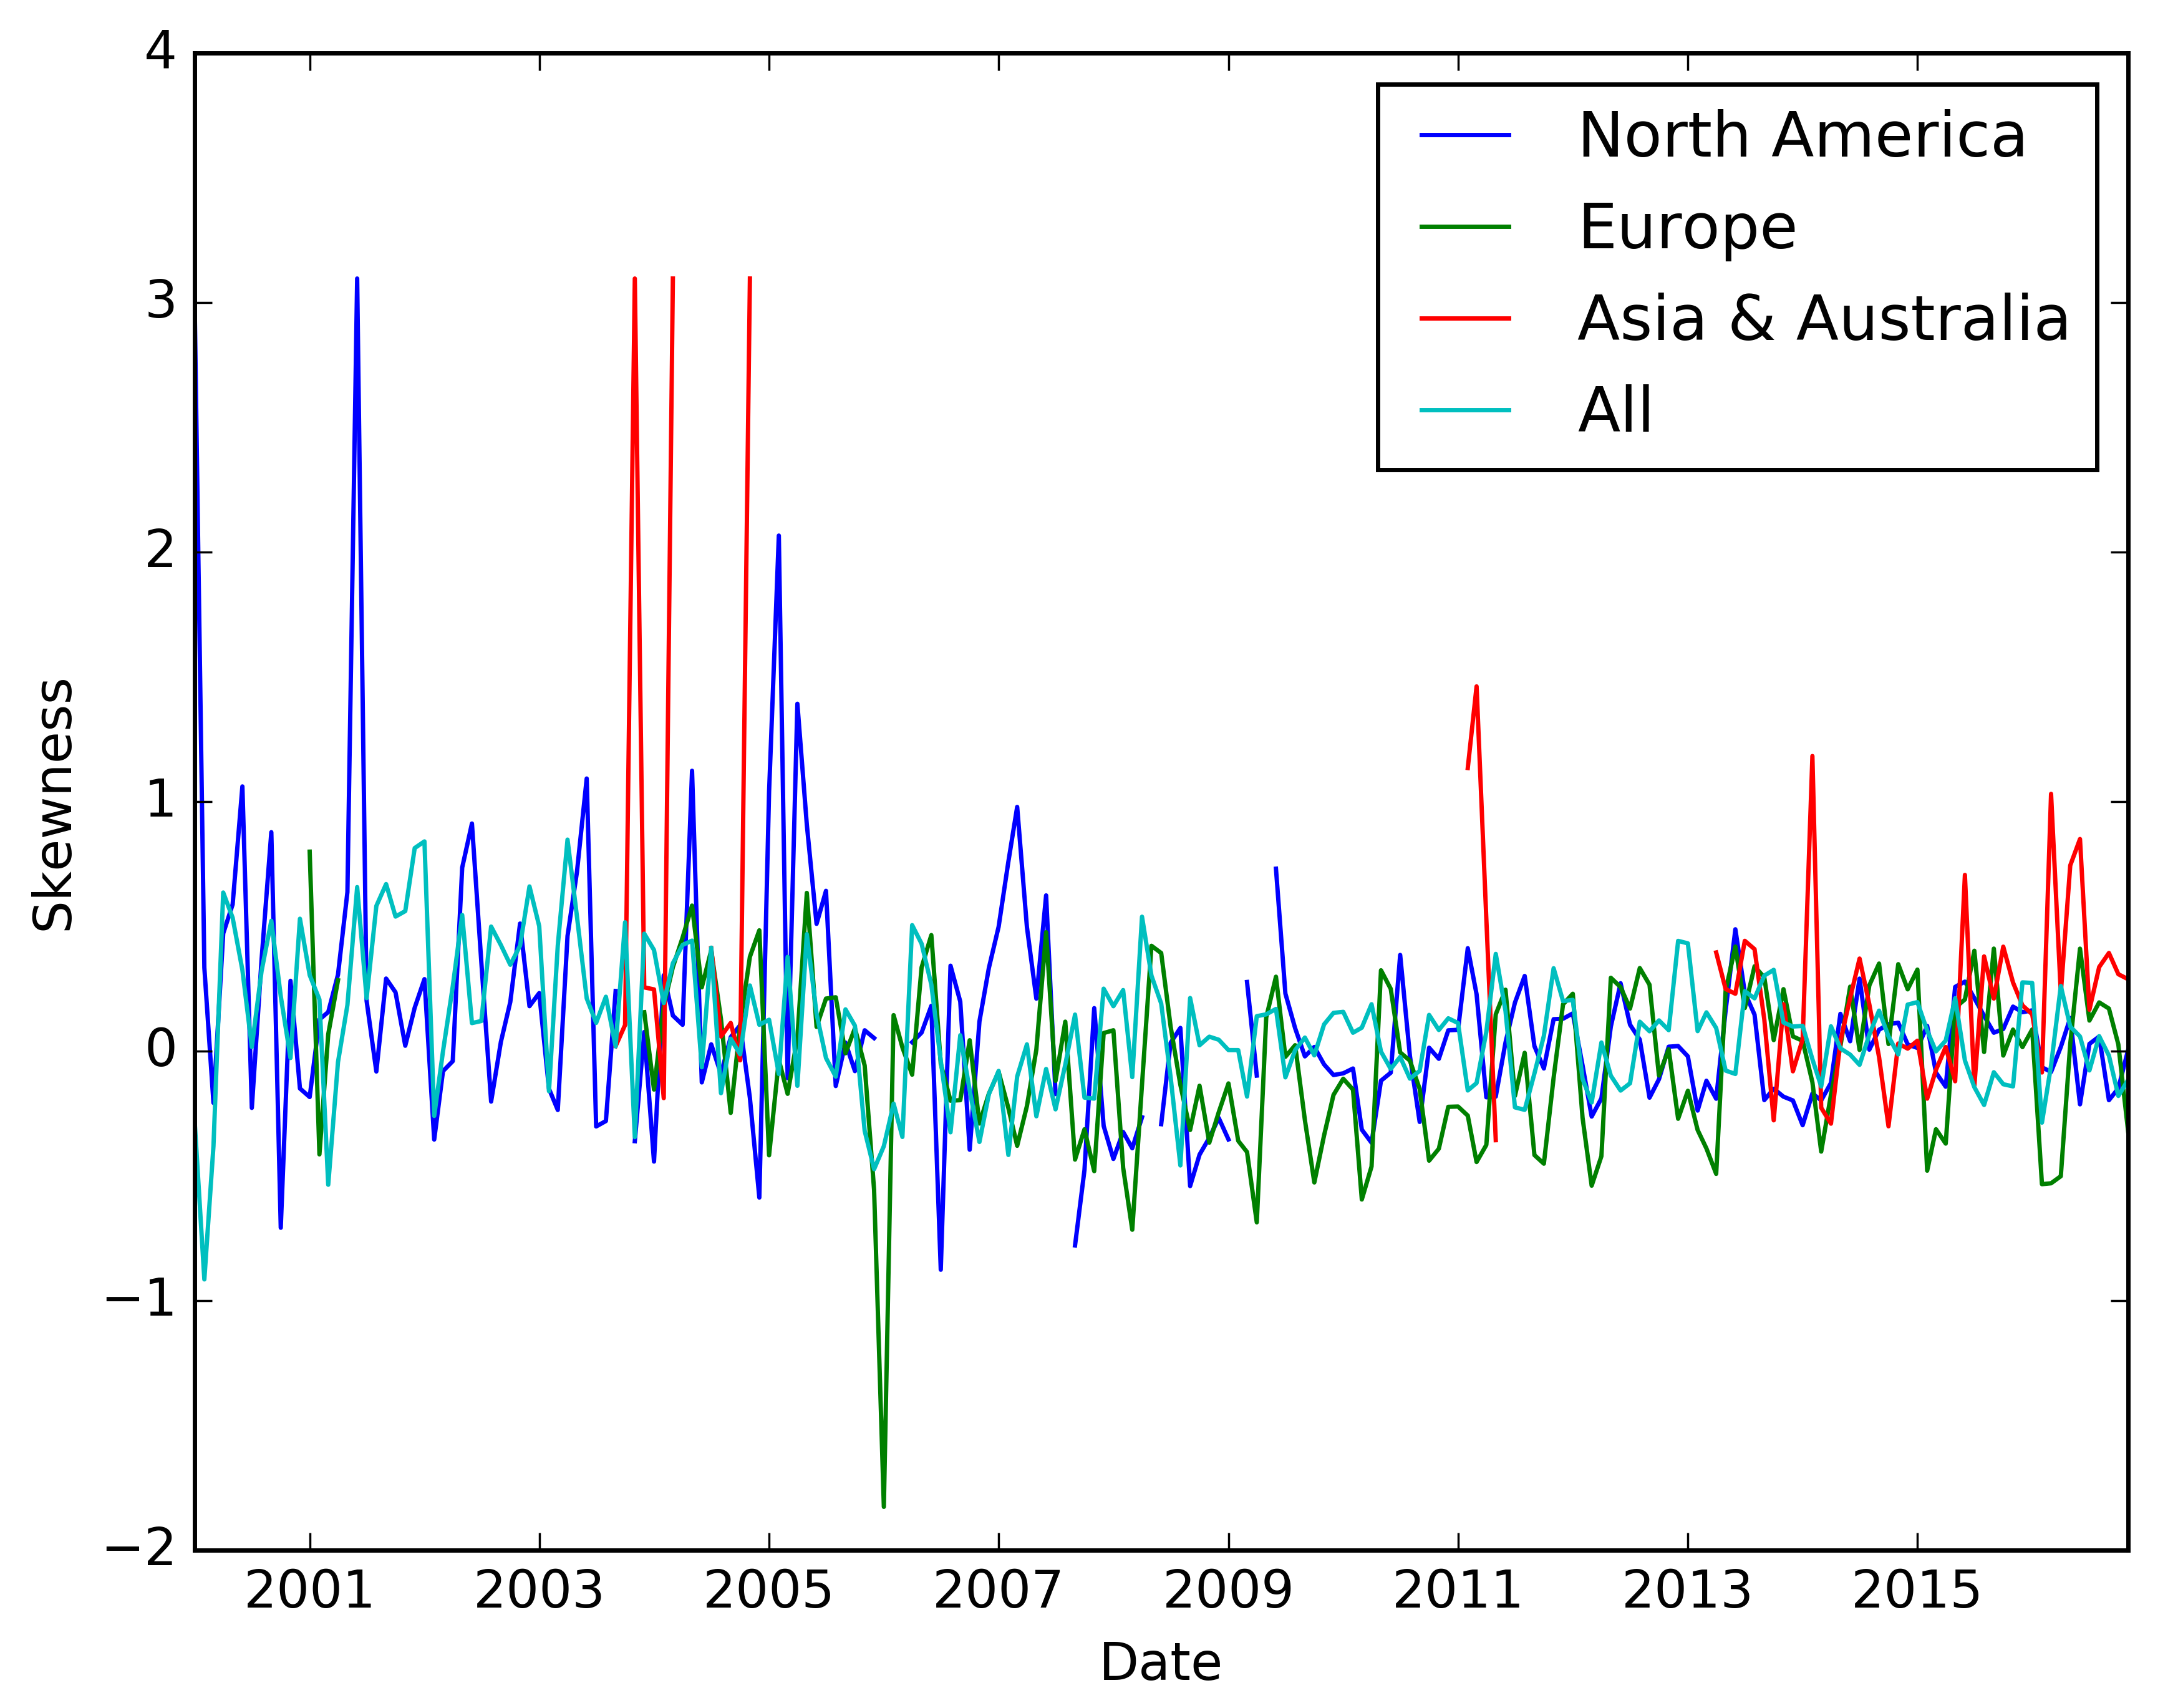
\includegraphics[width=\linewidth]{temporal/analyses/COMBINEDskew}
	\caption{Variation of skewness
		\label{fig:temp:skew}}
\end{figure}
\paragraph{Diurnal shift\\}
Between 2003 and 2007 there is a large amount of variation for observers in both Asia \& Australia, and North America. Towards more recent years, the variation is much smaller for all categories. The overall trend is not clear due to the large variation. Mostly, each category appears to fluctuate around certain values. For observers in Europe, this is $\sim$ 6, in Asia \& Australia the values fluctuate around $\sim$ 18, and in North America, around $\sim$12.
\begin{figure}[h!]
	\centering
	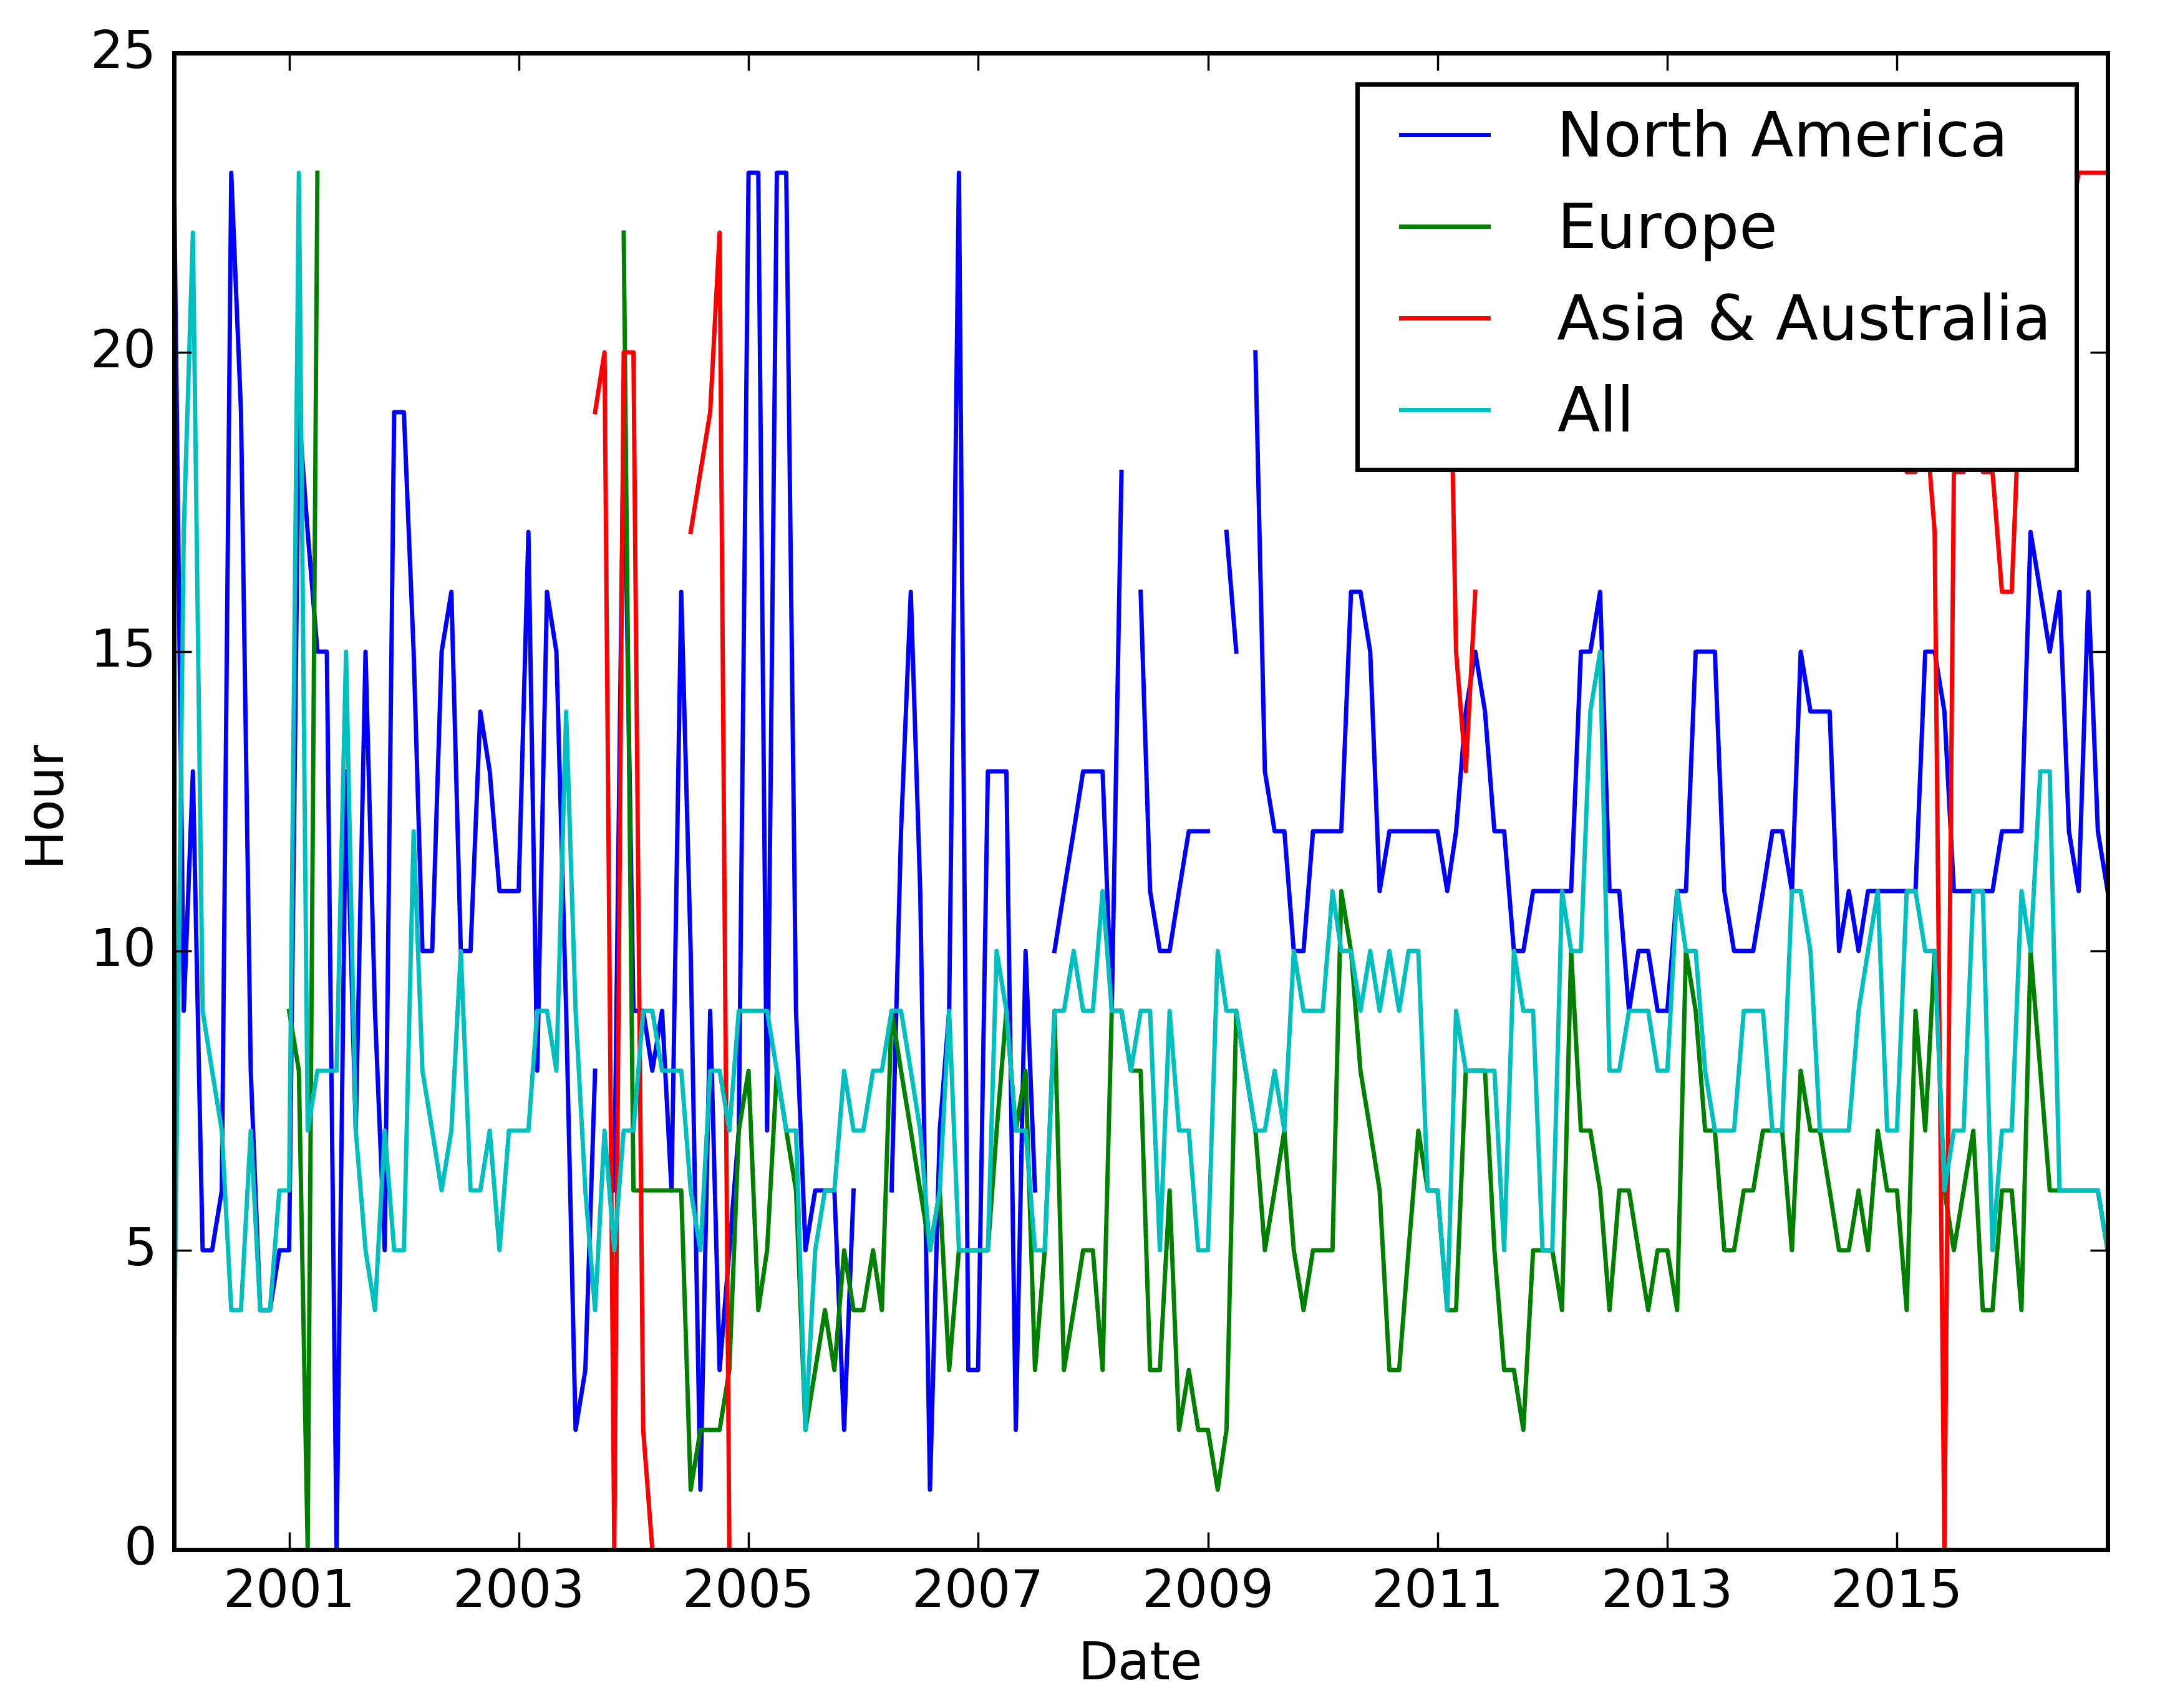
\includegraphics[width=\linewidth]{temporal/analyses/COMBINEDpeak}
	\caption{Variation of peak hour of diurnal shift
		\label{fig:temp:peak}}
\end{figure}
During the periods with the most fluctuation in figure~\ref{fig:temp:peak}, the sum of the parameter covariance, indicating how well a sine function fits the data, is greatest. The mean fit, across all observers, is relatively low throughout the years available, however there is again a noticeable increase between 2005 and 2010, which fits in with increases \& decreases in other analyses. The fit is closer to 0 in recent years, for all categories other than North America, though this category does decrease too.
\begin{figure}[h!]
	\centering
	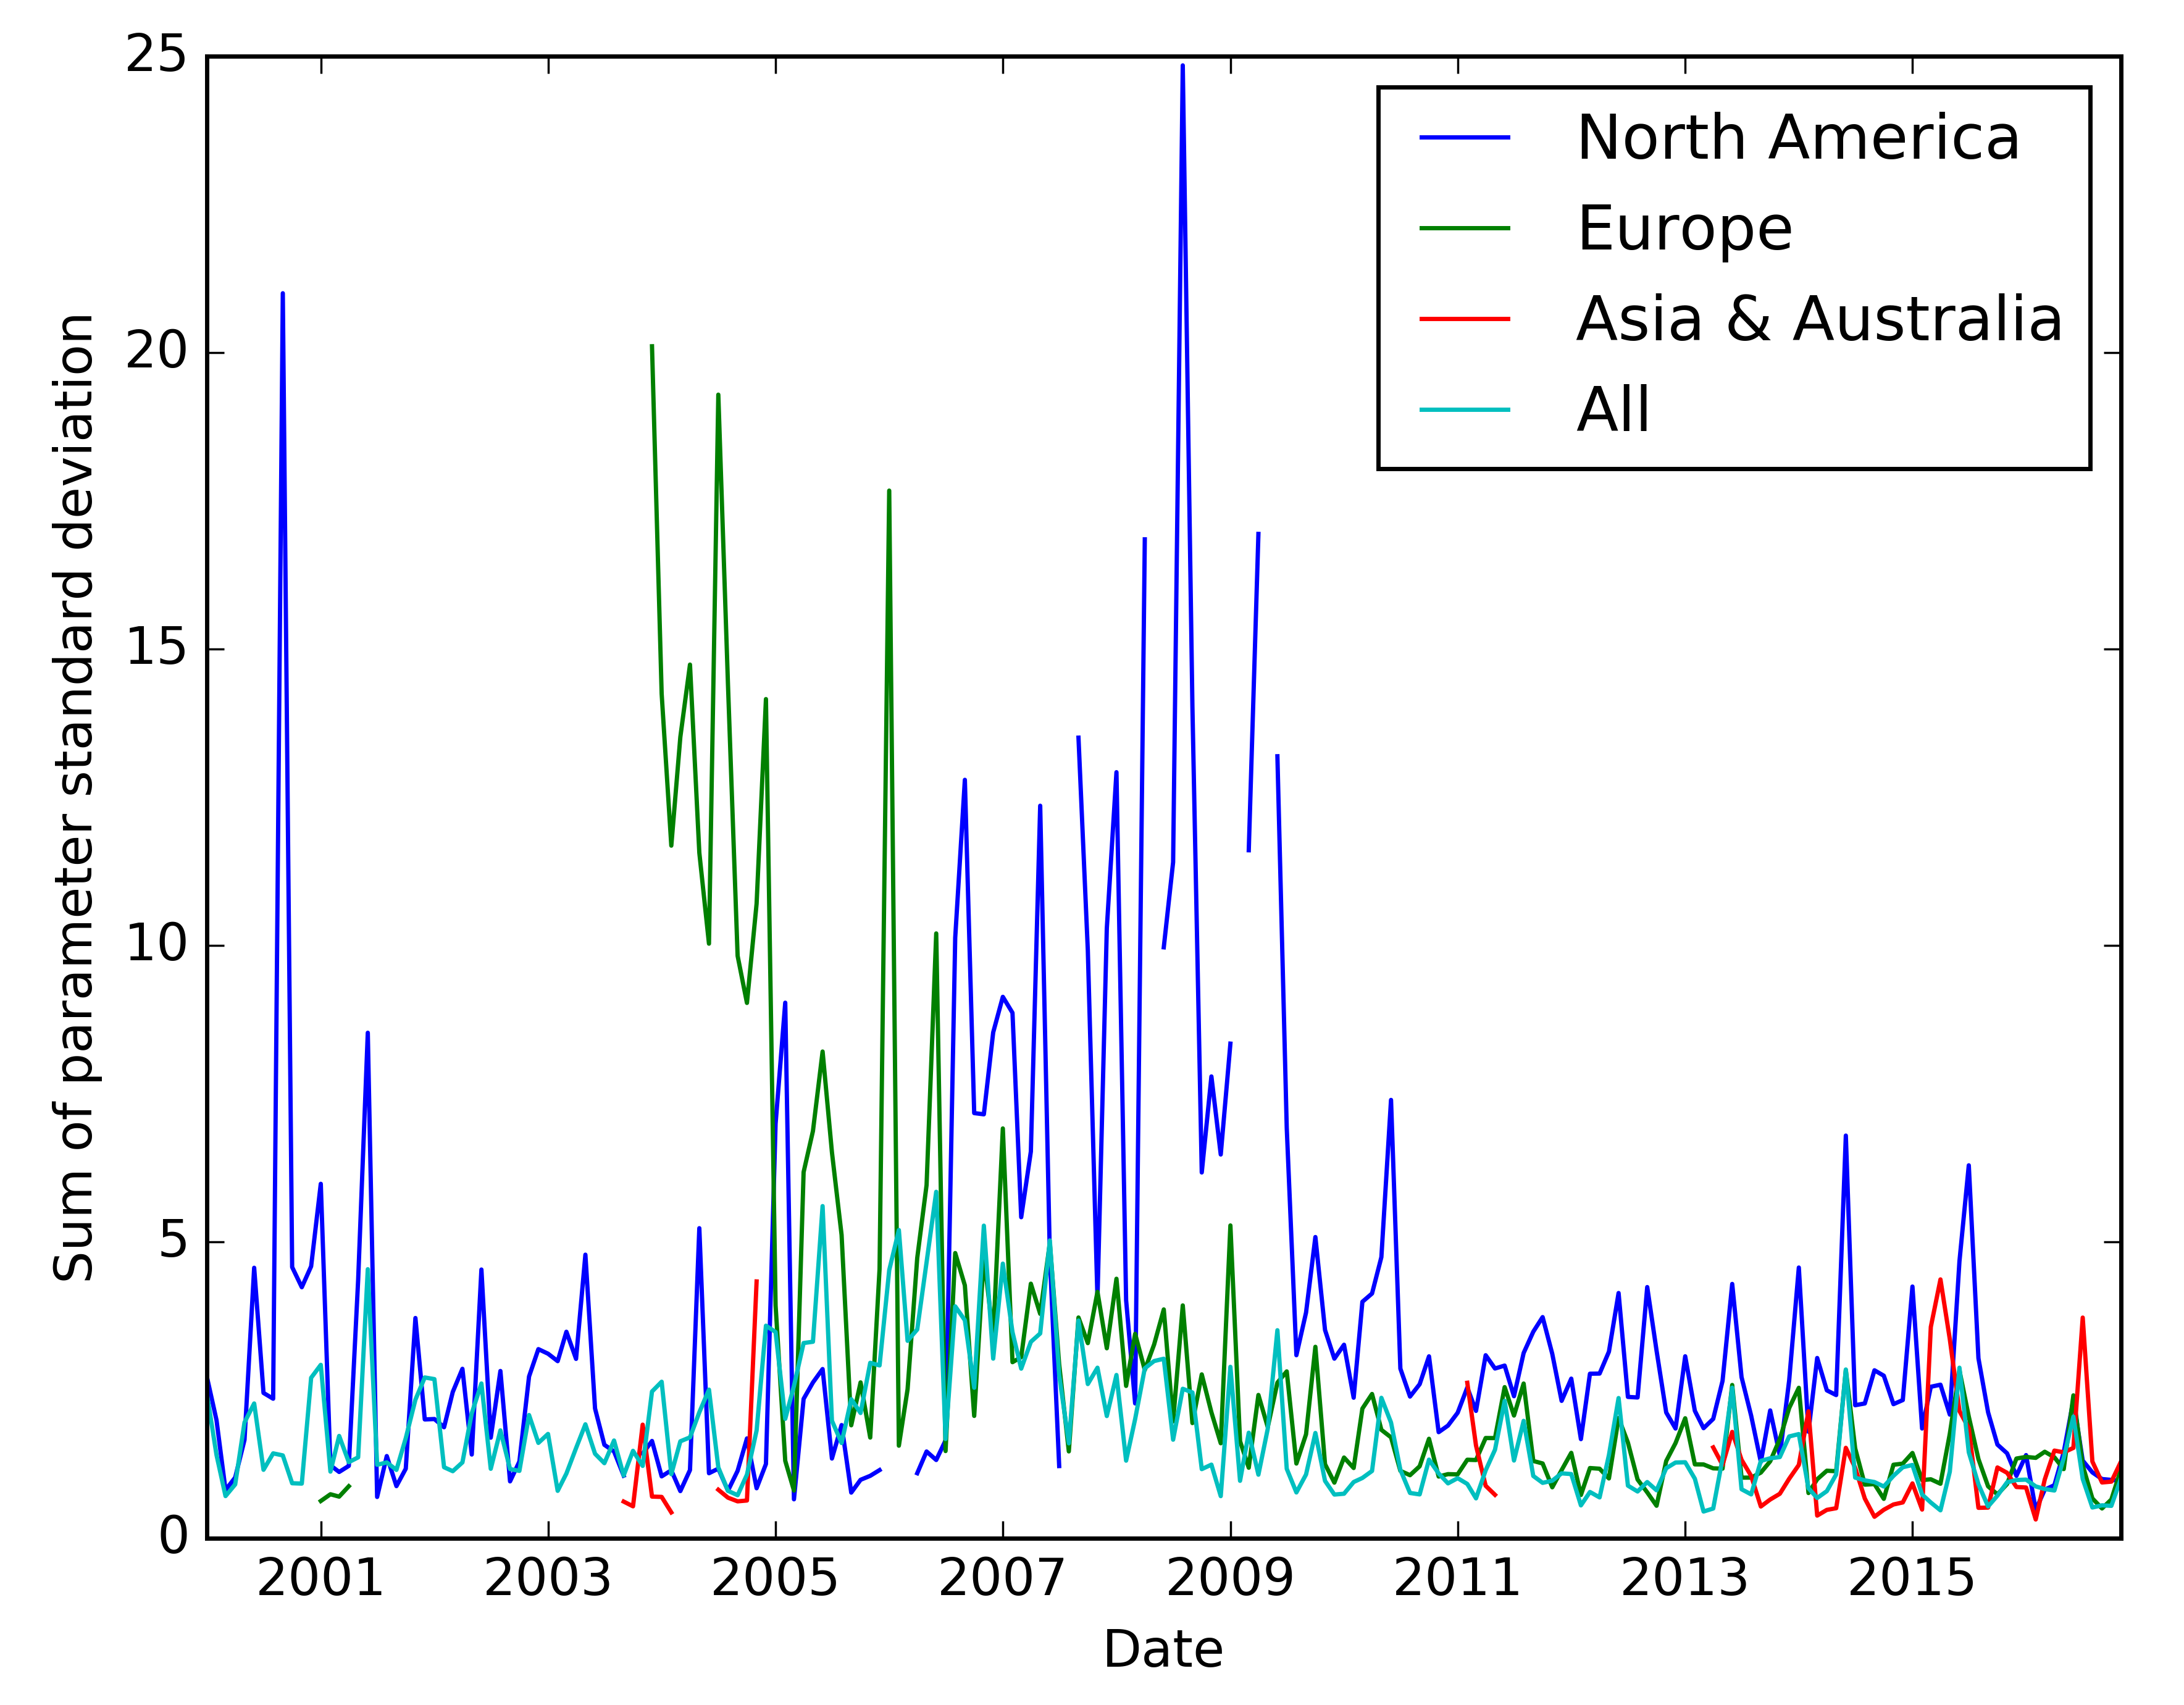
\includegraphics[width=\linewidth]{temporal/analyses/COMBINEDfit}
	\caption{Variation of fit to optimal sine function for diurnal shift
		\label{fig:temp:fit}}
\end{figure}

\subsection{Monthly scale variation}
The variation over the course of a month is shown in figure~\ref{fig:temp:day}. There is no overall trend throughout a month. There is no overall increase or decrease, though there is a slight increase around the 13th day in the month.
\begin{figure}[h!]
	\centering
	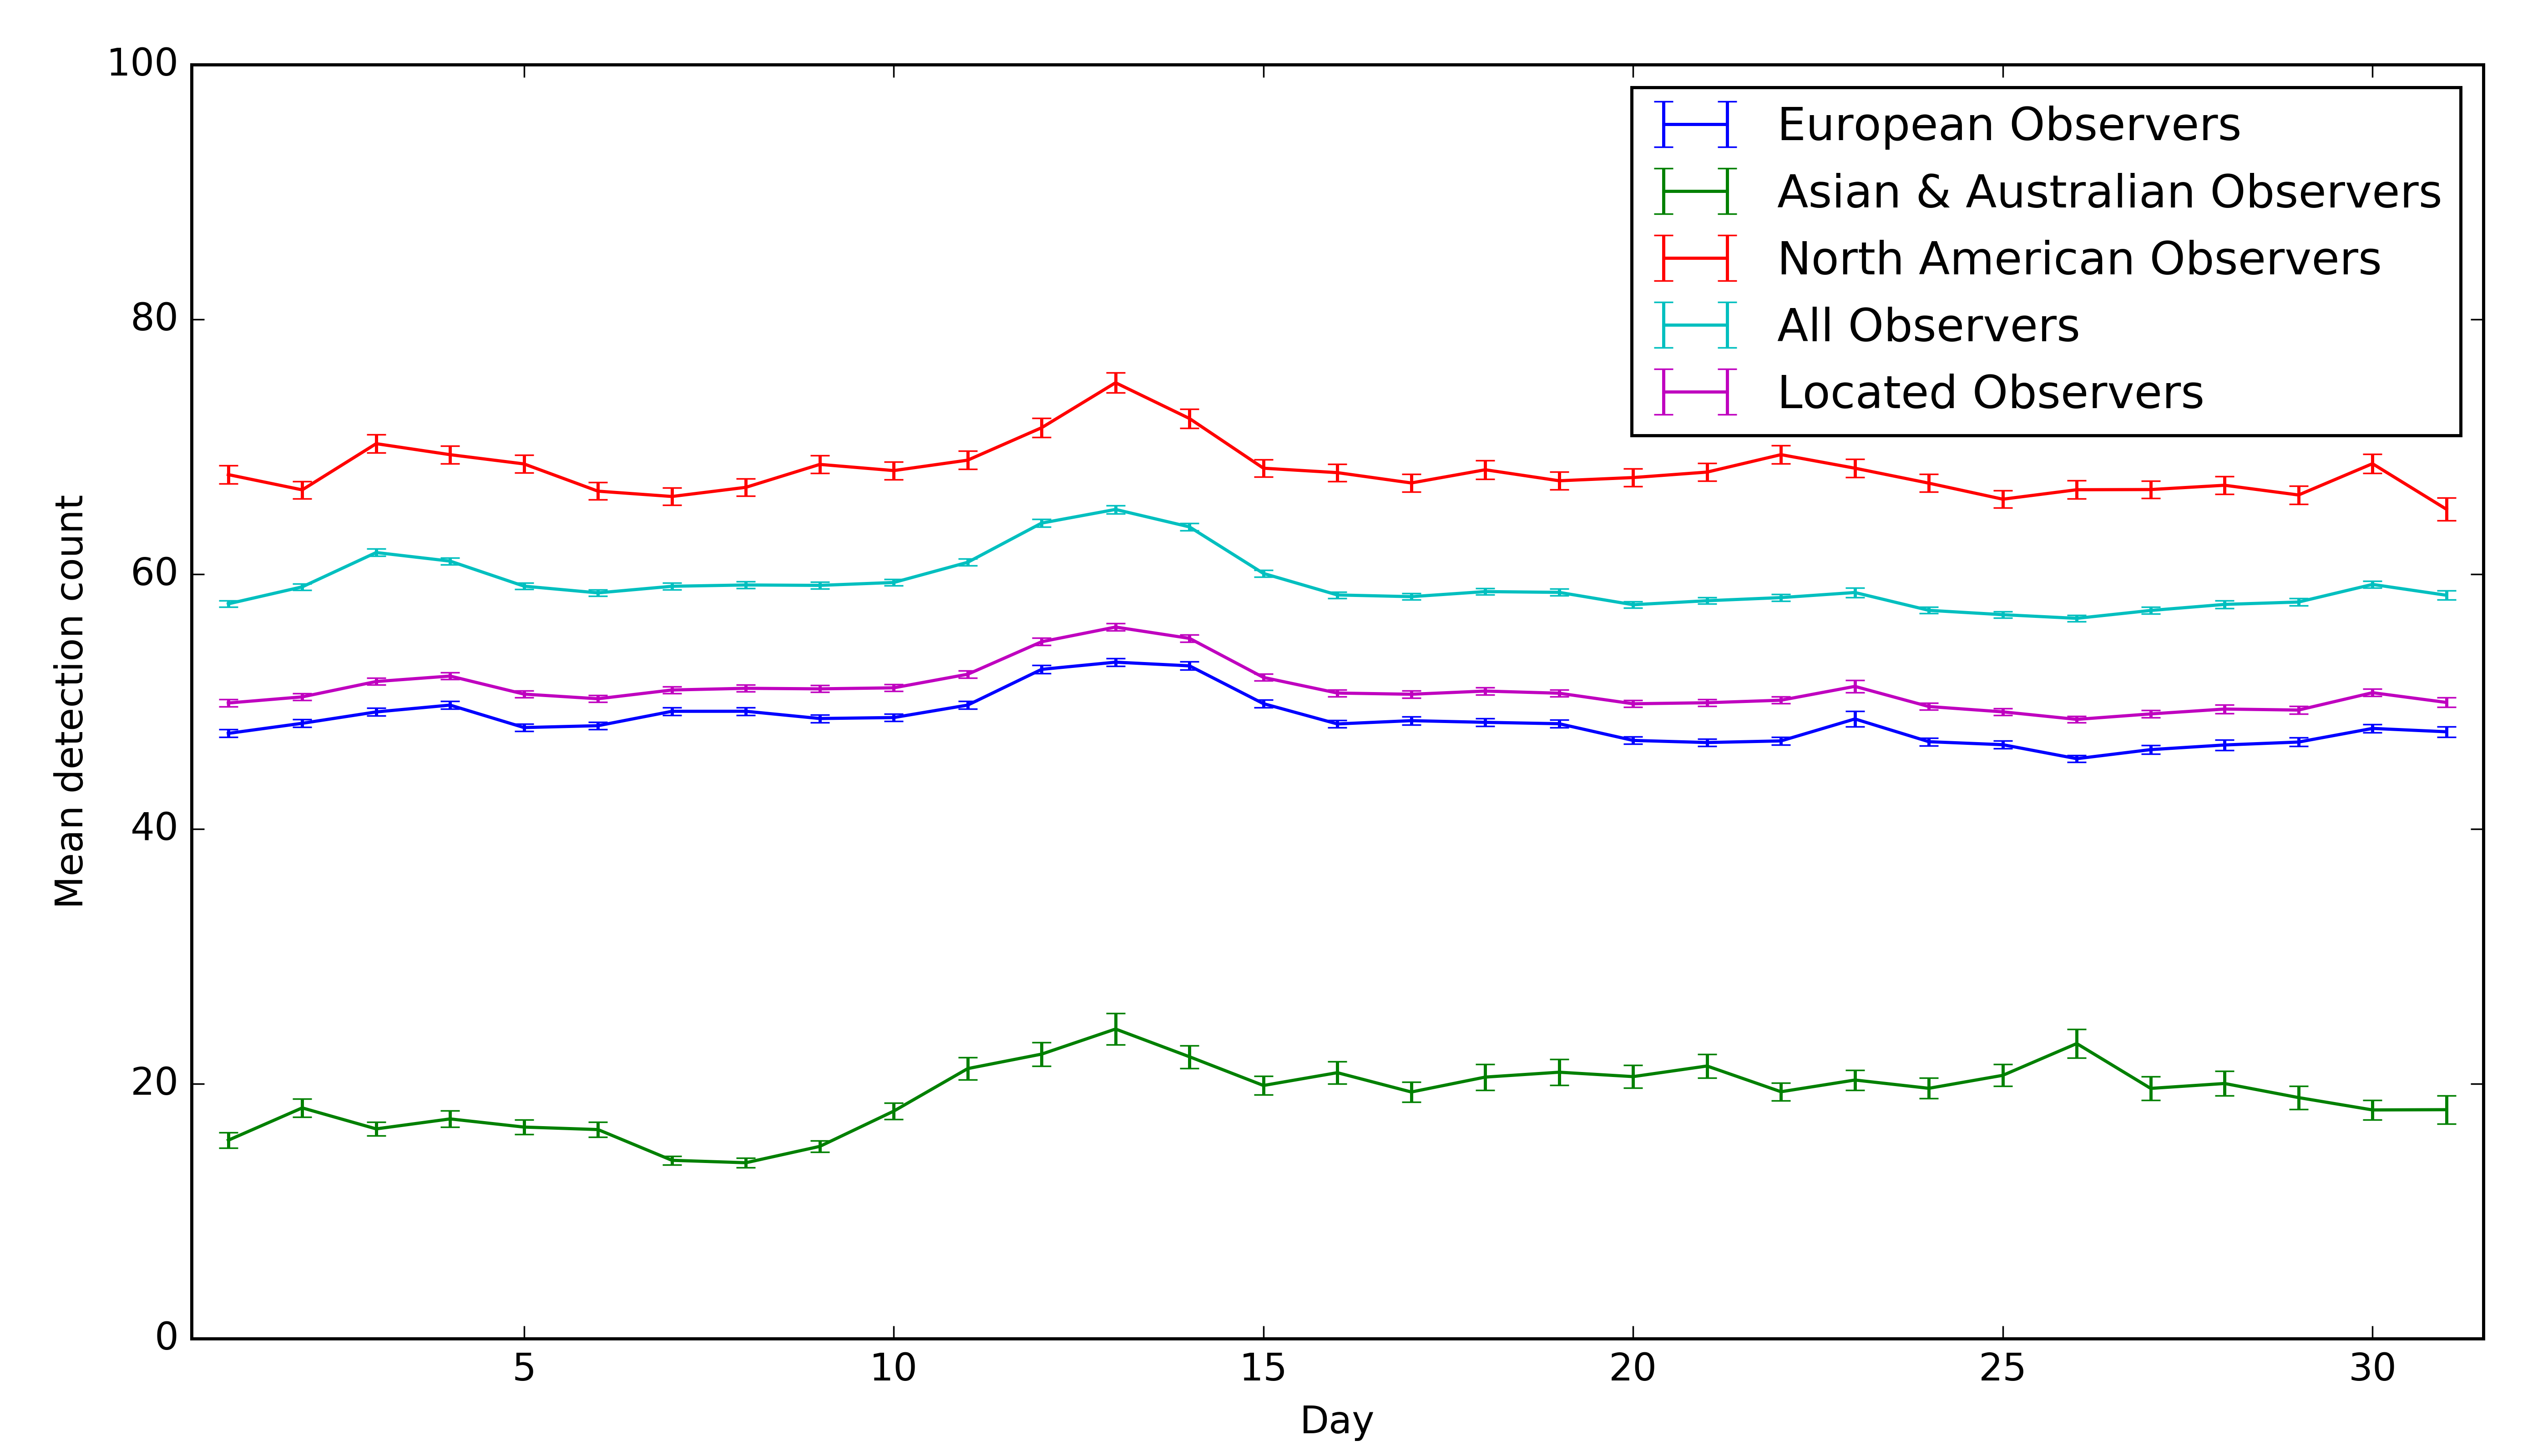
\includegraphics[width=\linewidth]{temporal/Dcombined}
	\caption{Variation in mean hourly detection count over a month
		\label{fig:temp:day}}
\end{figure}
\subsection{Annual scale variation}
There is a clear increase from the beginning of a year to the end, for all categories other than Asia \& Australia. From January to February, there is a small decrease, followed by an increase until June. This is followed by a small decrease of $\sim$ 10 detections an hour, until August. The mean hourly detection count then remains roughly constant until the end of the year. This is the same for all categories other than Asia \& Australia. For this category, there is an increase in April and May, and then a decrease and a constant hourly count for the rest of the year.
\begin{figure}[h!]
	\centering
	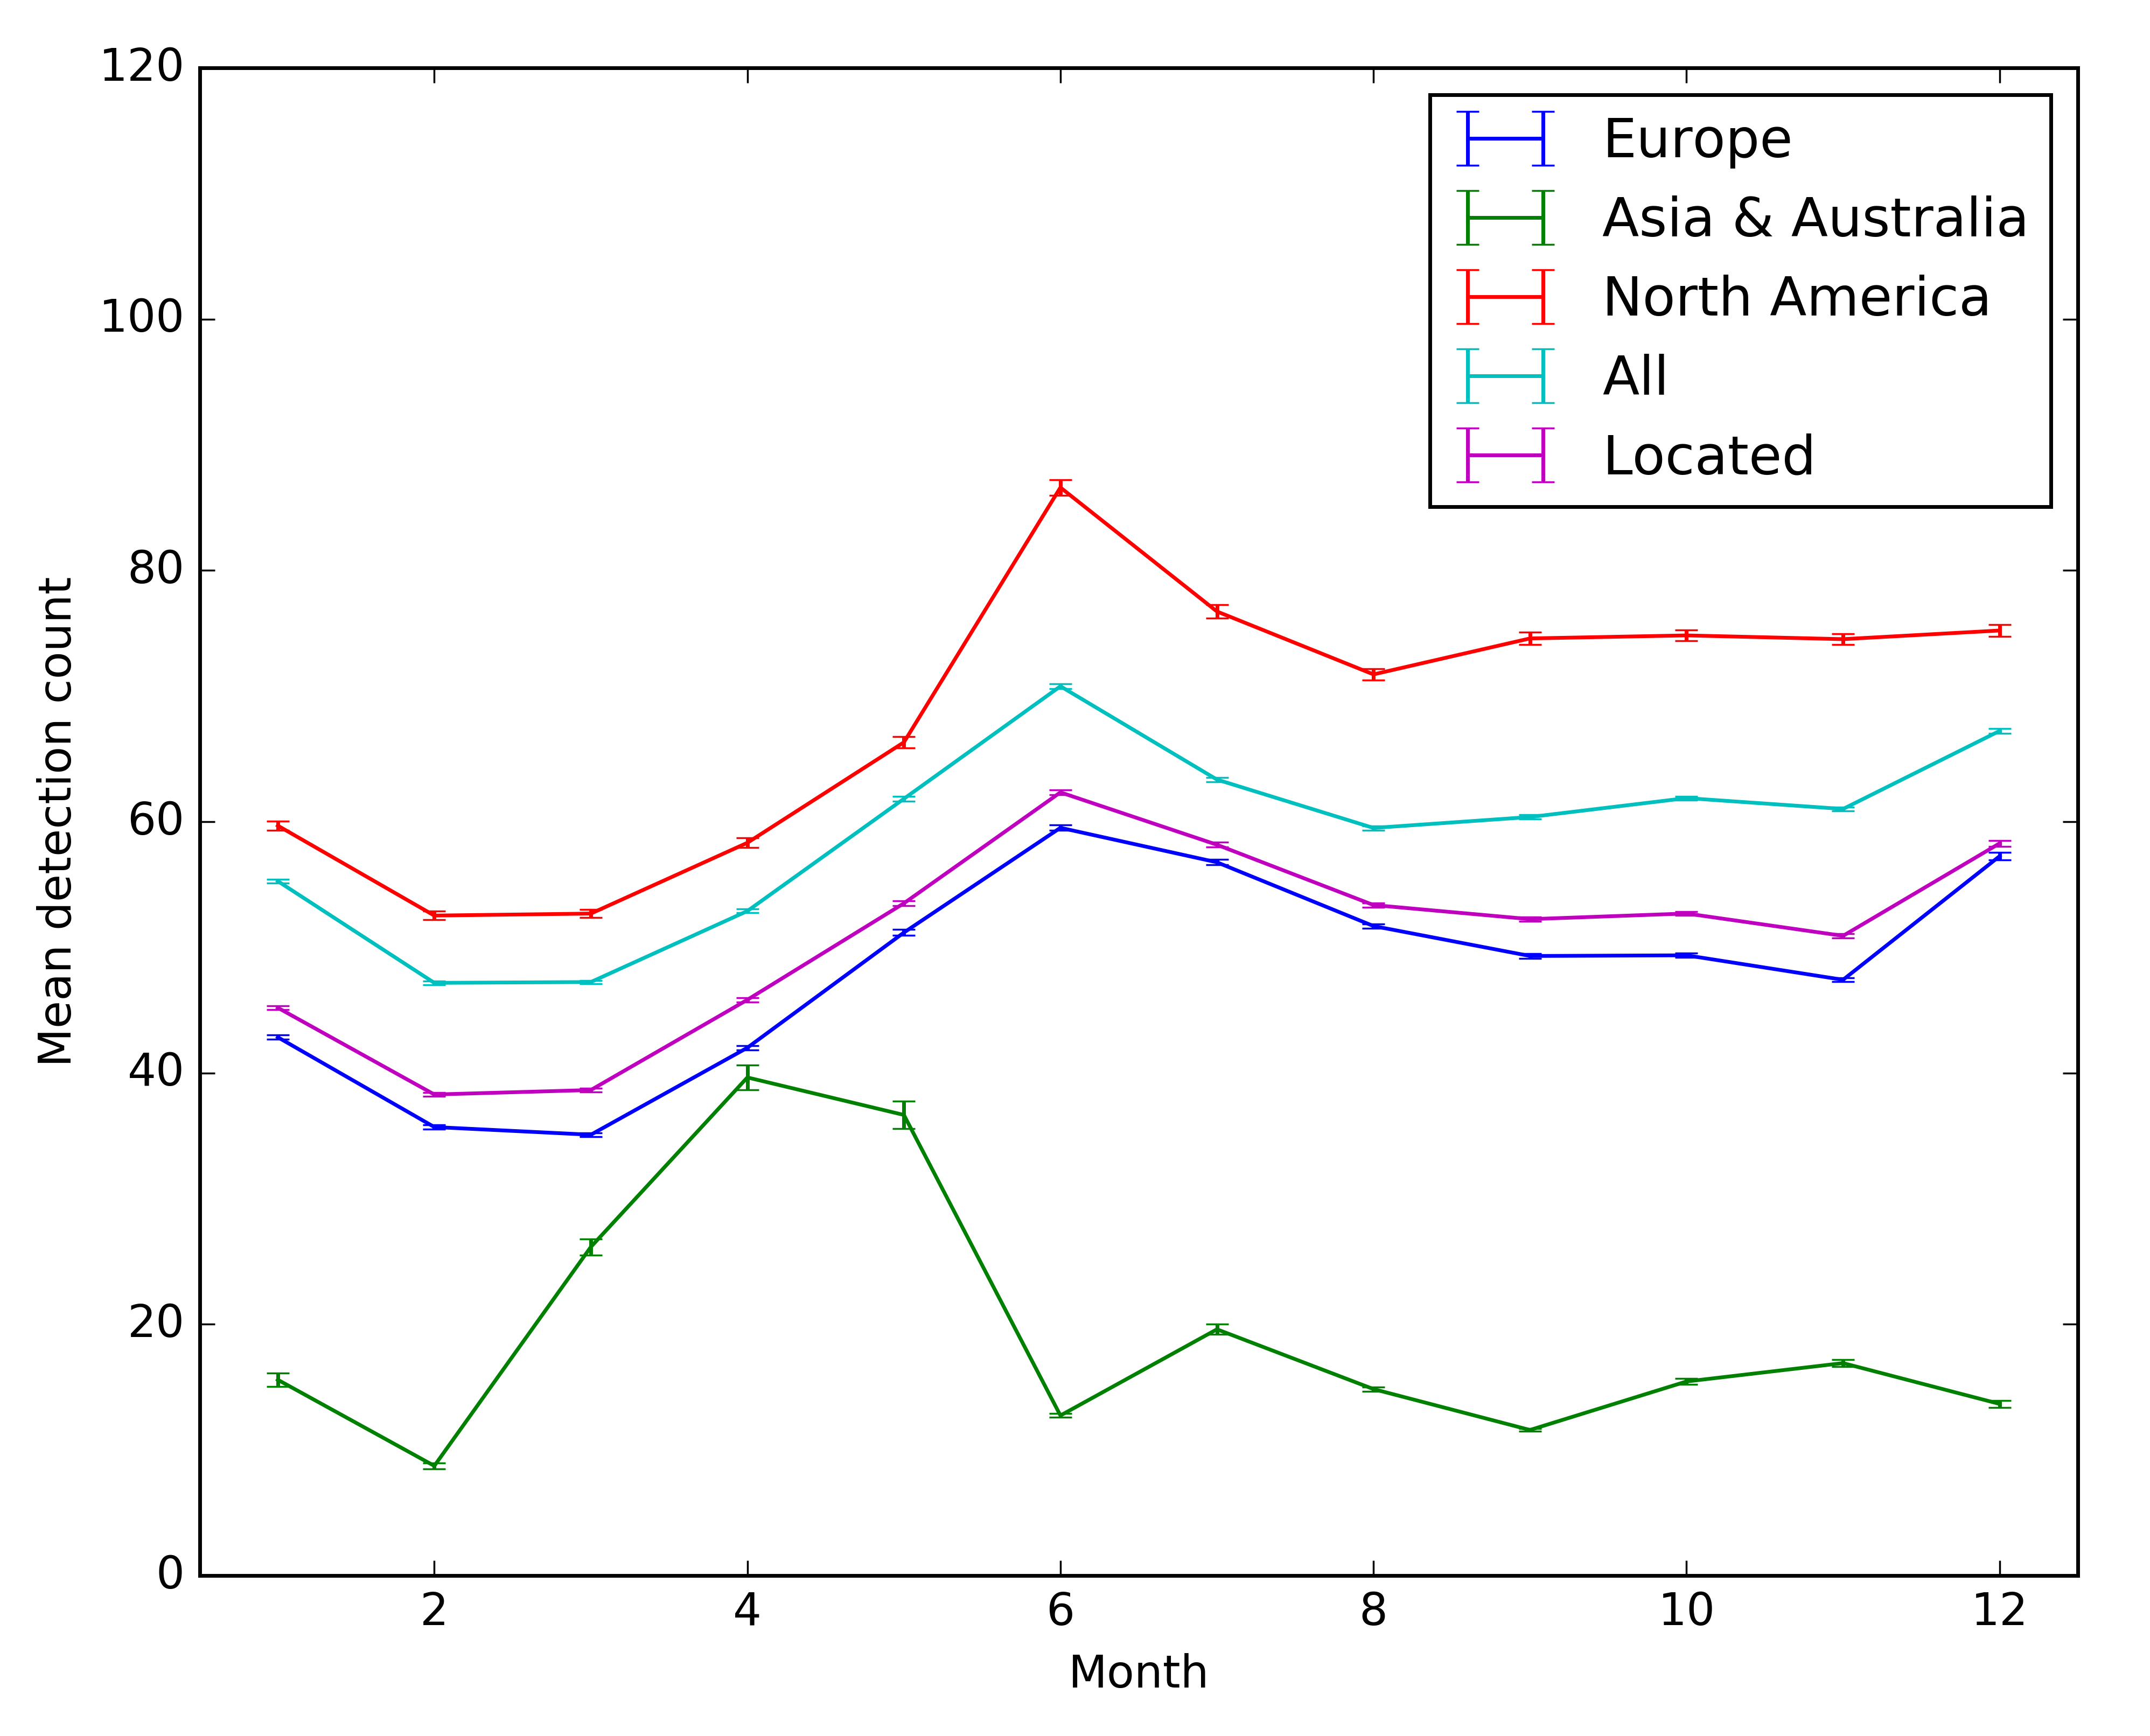
\includegraphics[width=\linewidth]{temporal/Mcombined}
	\caption{Variation in mean hourly detection count over a year
		\label{fig:temp:month}}
\end{figure}
\subsection{Variation since 2000}
Between 2003 and 2011 there is a dramatic increase in the mean hourly detection count across an entire year. This increase is on the order of $\sim$ 2 times, from $\sim$ 60 to $\sim$ 120. This increase is out of phase by 1 year for the North American category. Once the count returns to $\sim$ 60, it remains there from 2011 to 2016. There is no data available for the Asia \& Australia category for the maximum period so it is not known if the same increase is seen, however the category containing observers from the entire world exhibits the increase. Whilst the North American category has another peak in 2003, the standard error is much larger.
\begin{figure}[h!]
	\centering
	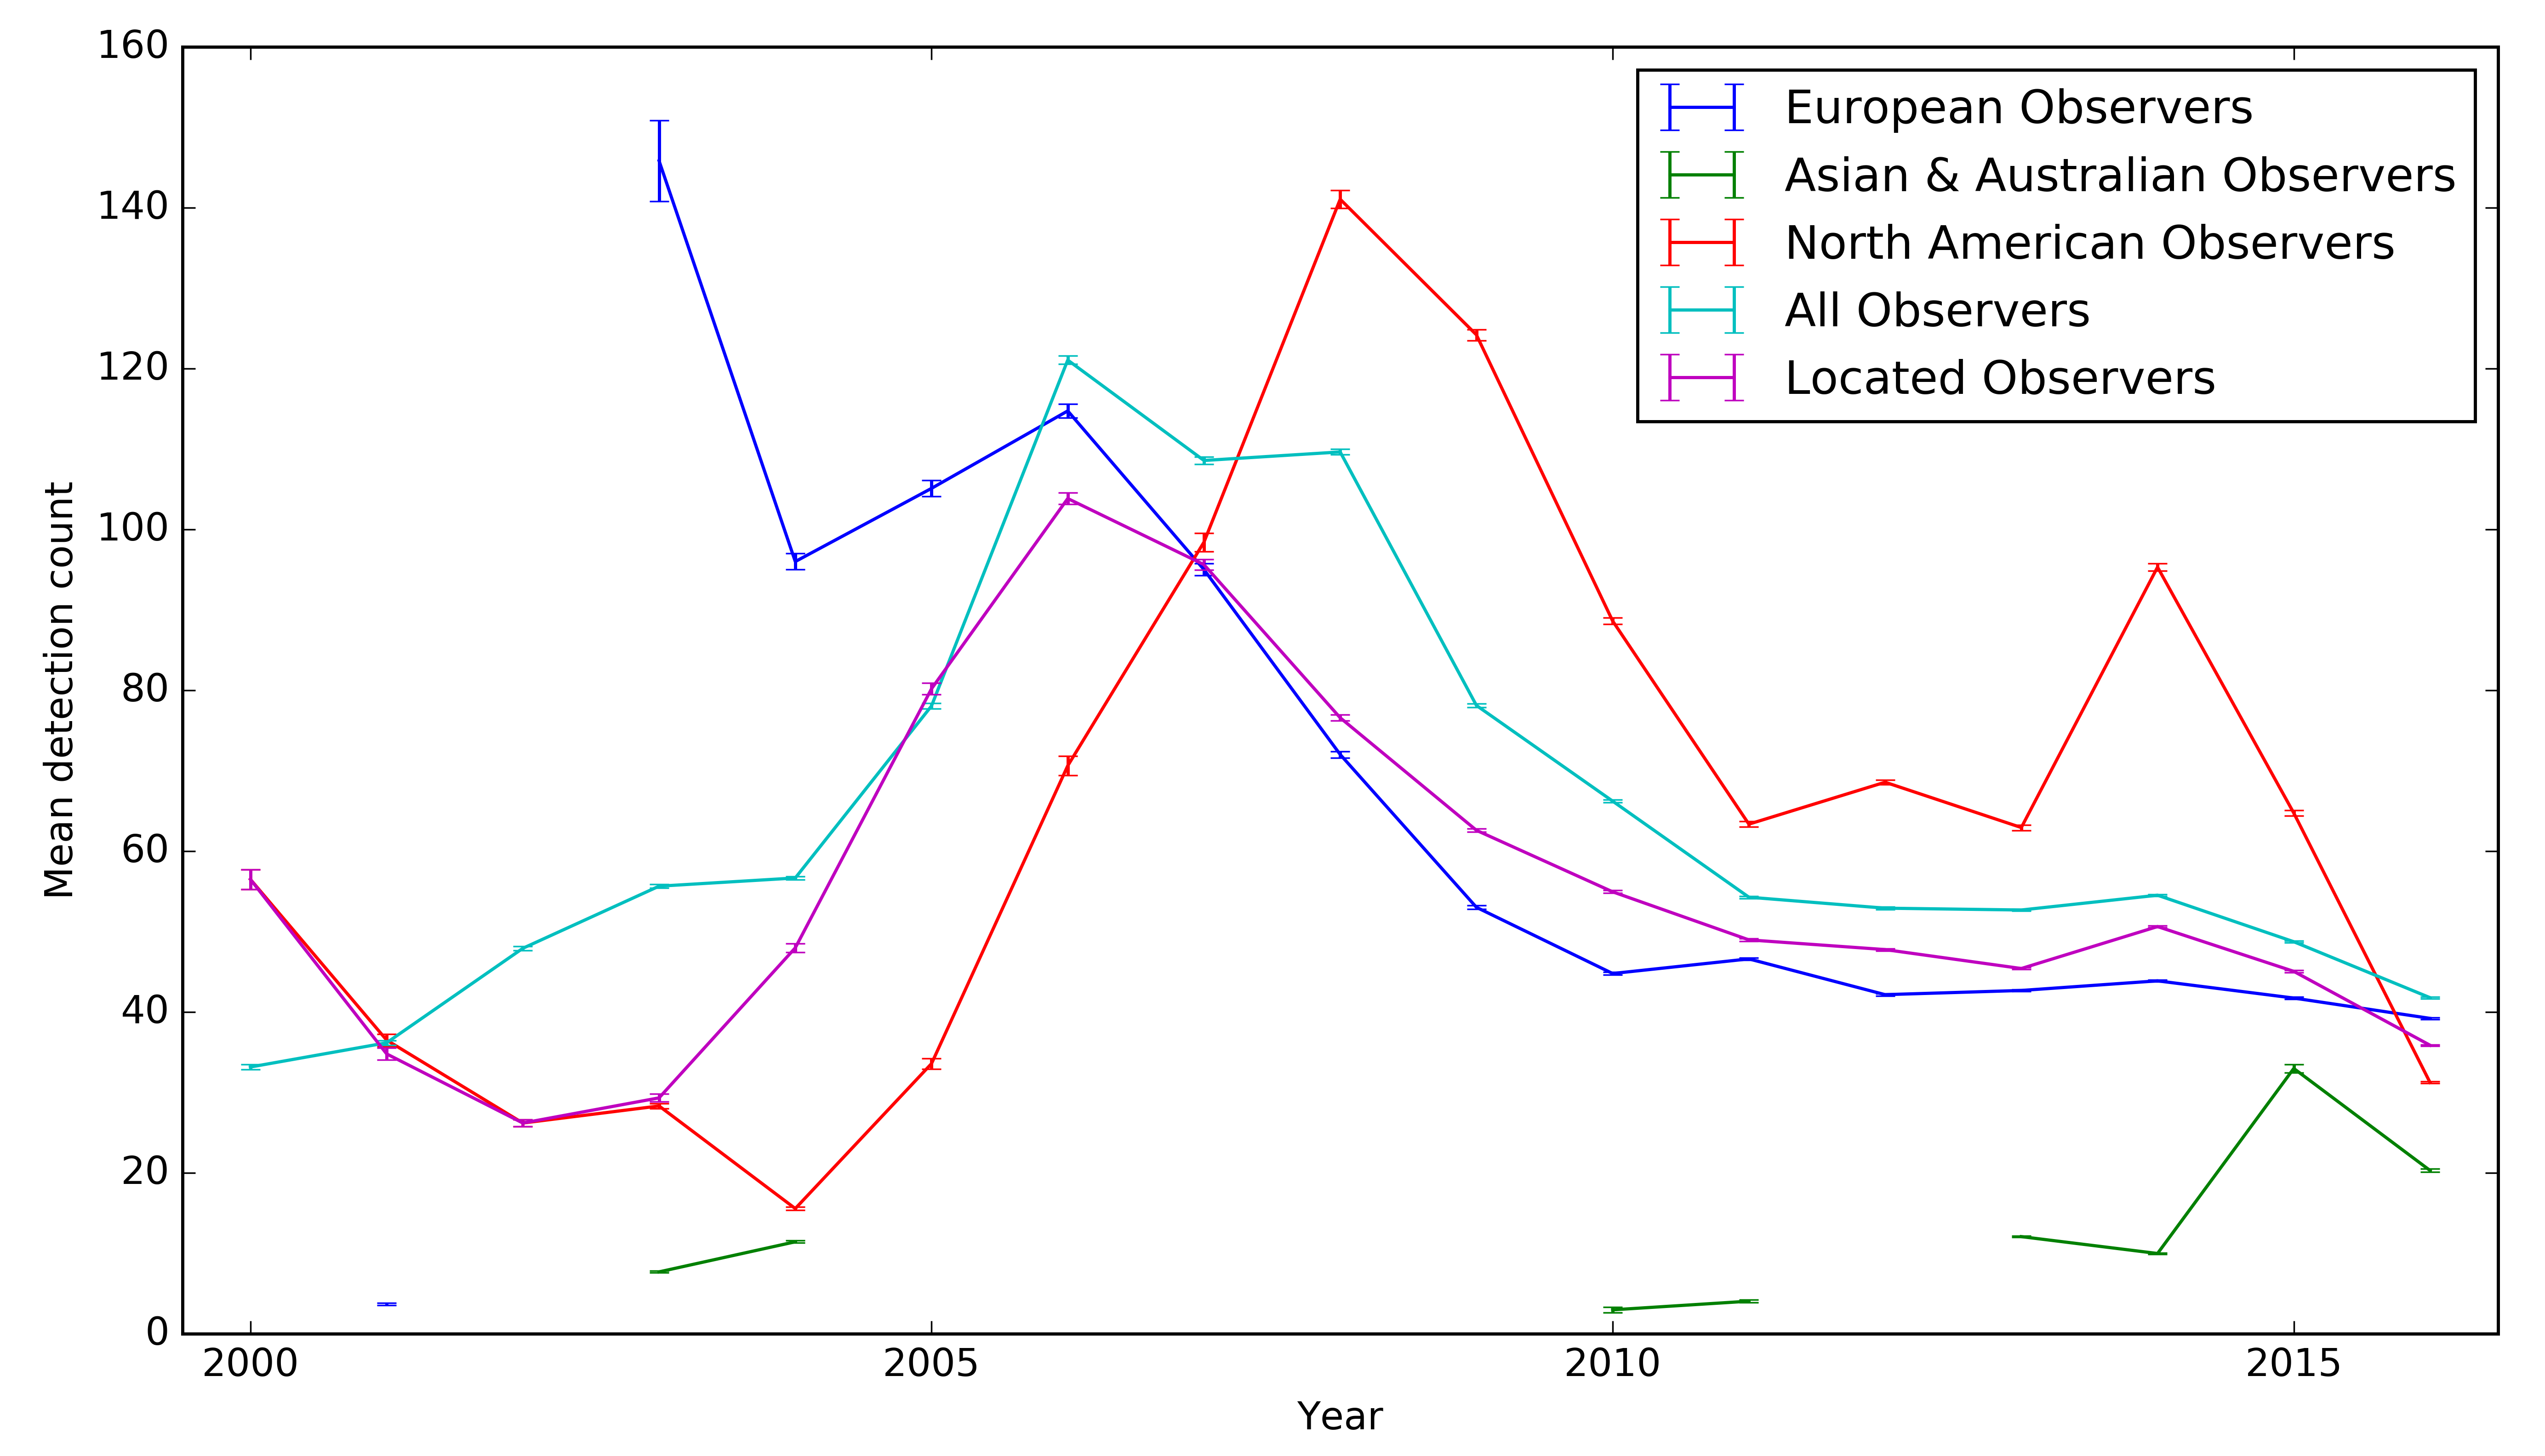
\includegraphics[width=\linewidth]{temporal/Ycombined}
	\caption{Variation in mean hourly detection count since 2000 by year
		\label{fig:temp:year}}
\end{figure}
Figure~\ref{fig:temp:yearmonth} shows the same data as figure~\ref{fig:temp:year} but on a finer resolution: for each month of each year available. The same increase is seen as before, though it is clear there there is much more variation between 2004 and 2011, as noted in section~\ref{par:err}. It is clear, from 2011 onwards, that there is a periodic variation each year, with a greater hourly detection count in the middle of the year.
\begin{figure}[h!]
	\centering
	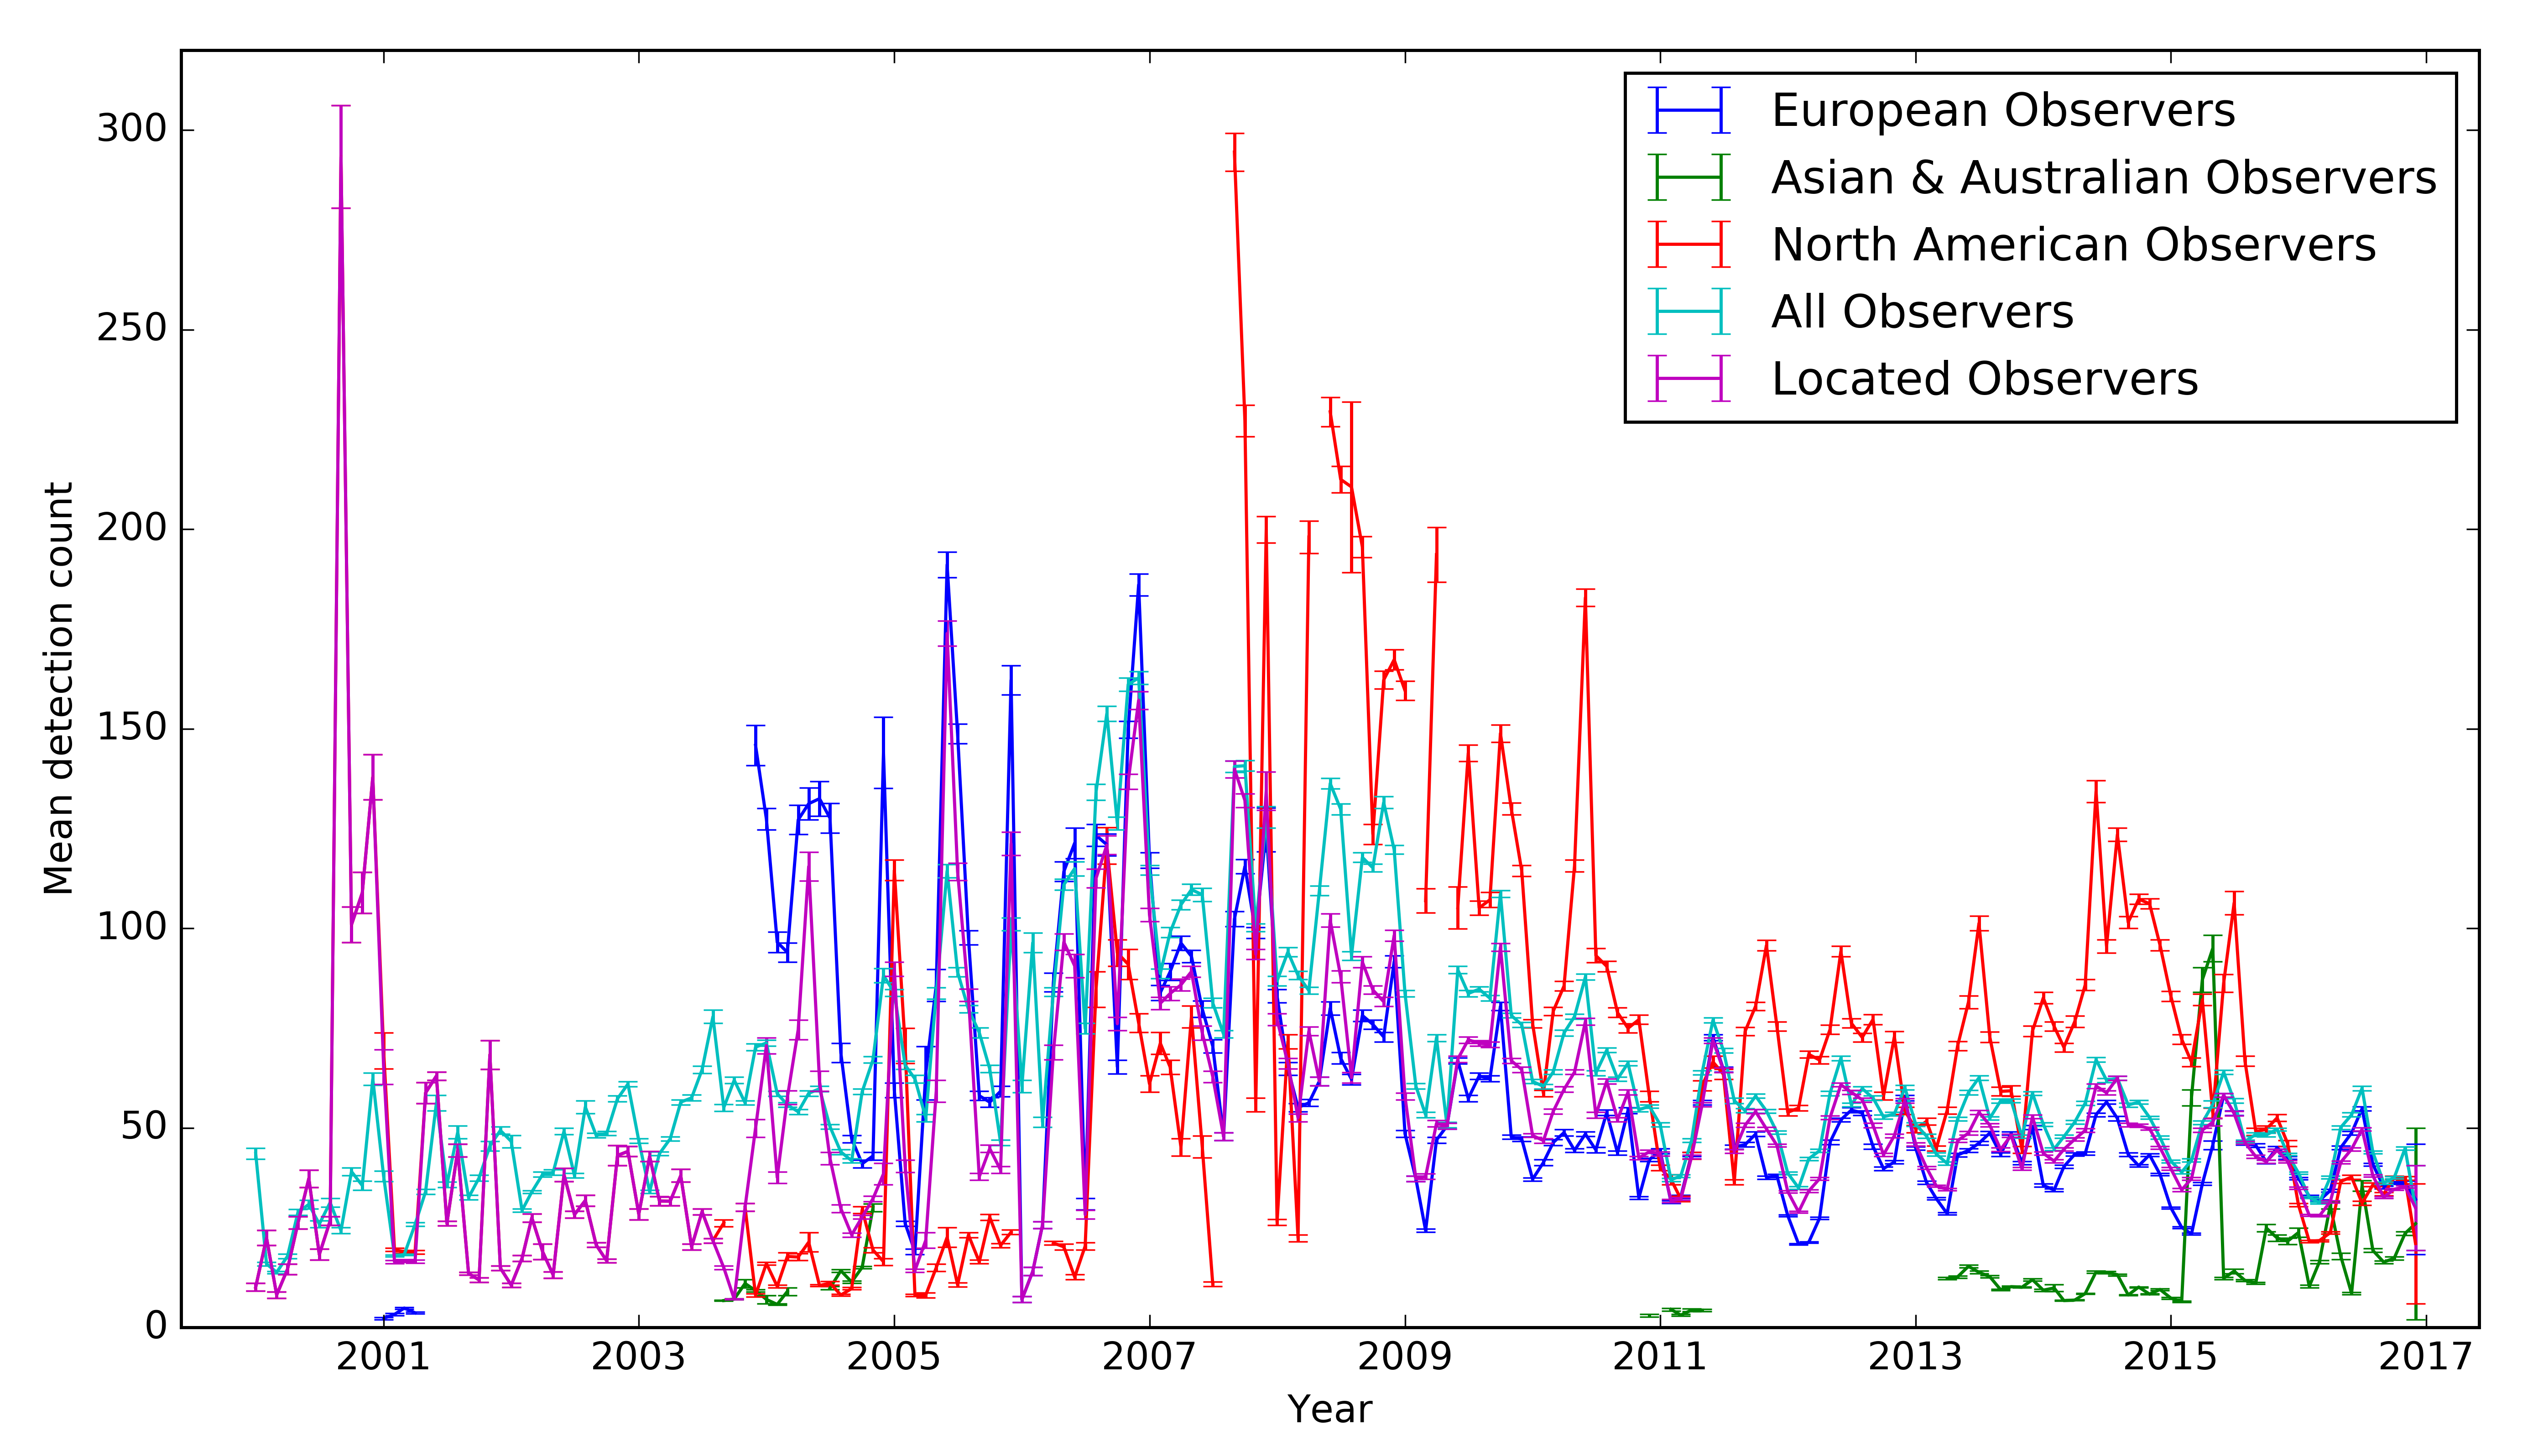
\includegraphics[width=\linewidth]{temporal/YMcombined}
	\caption{Variation in mean hourly detection count since 2000 by year and month
		\label{fig:temp:yearmonth}}
\end{figure}
\paragraph{Daytime vs. night-time rates\\}
In light of the correlation between the solar minimum and the maximum detection counts, I carried out a paired t-test to determine if there is a significant difference between the mean hourly detection counts when considering only daytime values, and night-time values. There is no significant difference between daytime and night-time (1\% significance level). 
\begin{figure*}[h!]
	\centering
	\begin{subfigure}[bh!]{0.475\textwidth}
		\centering
		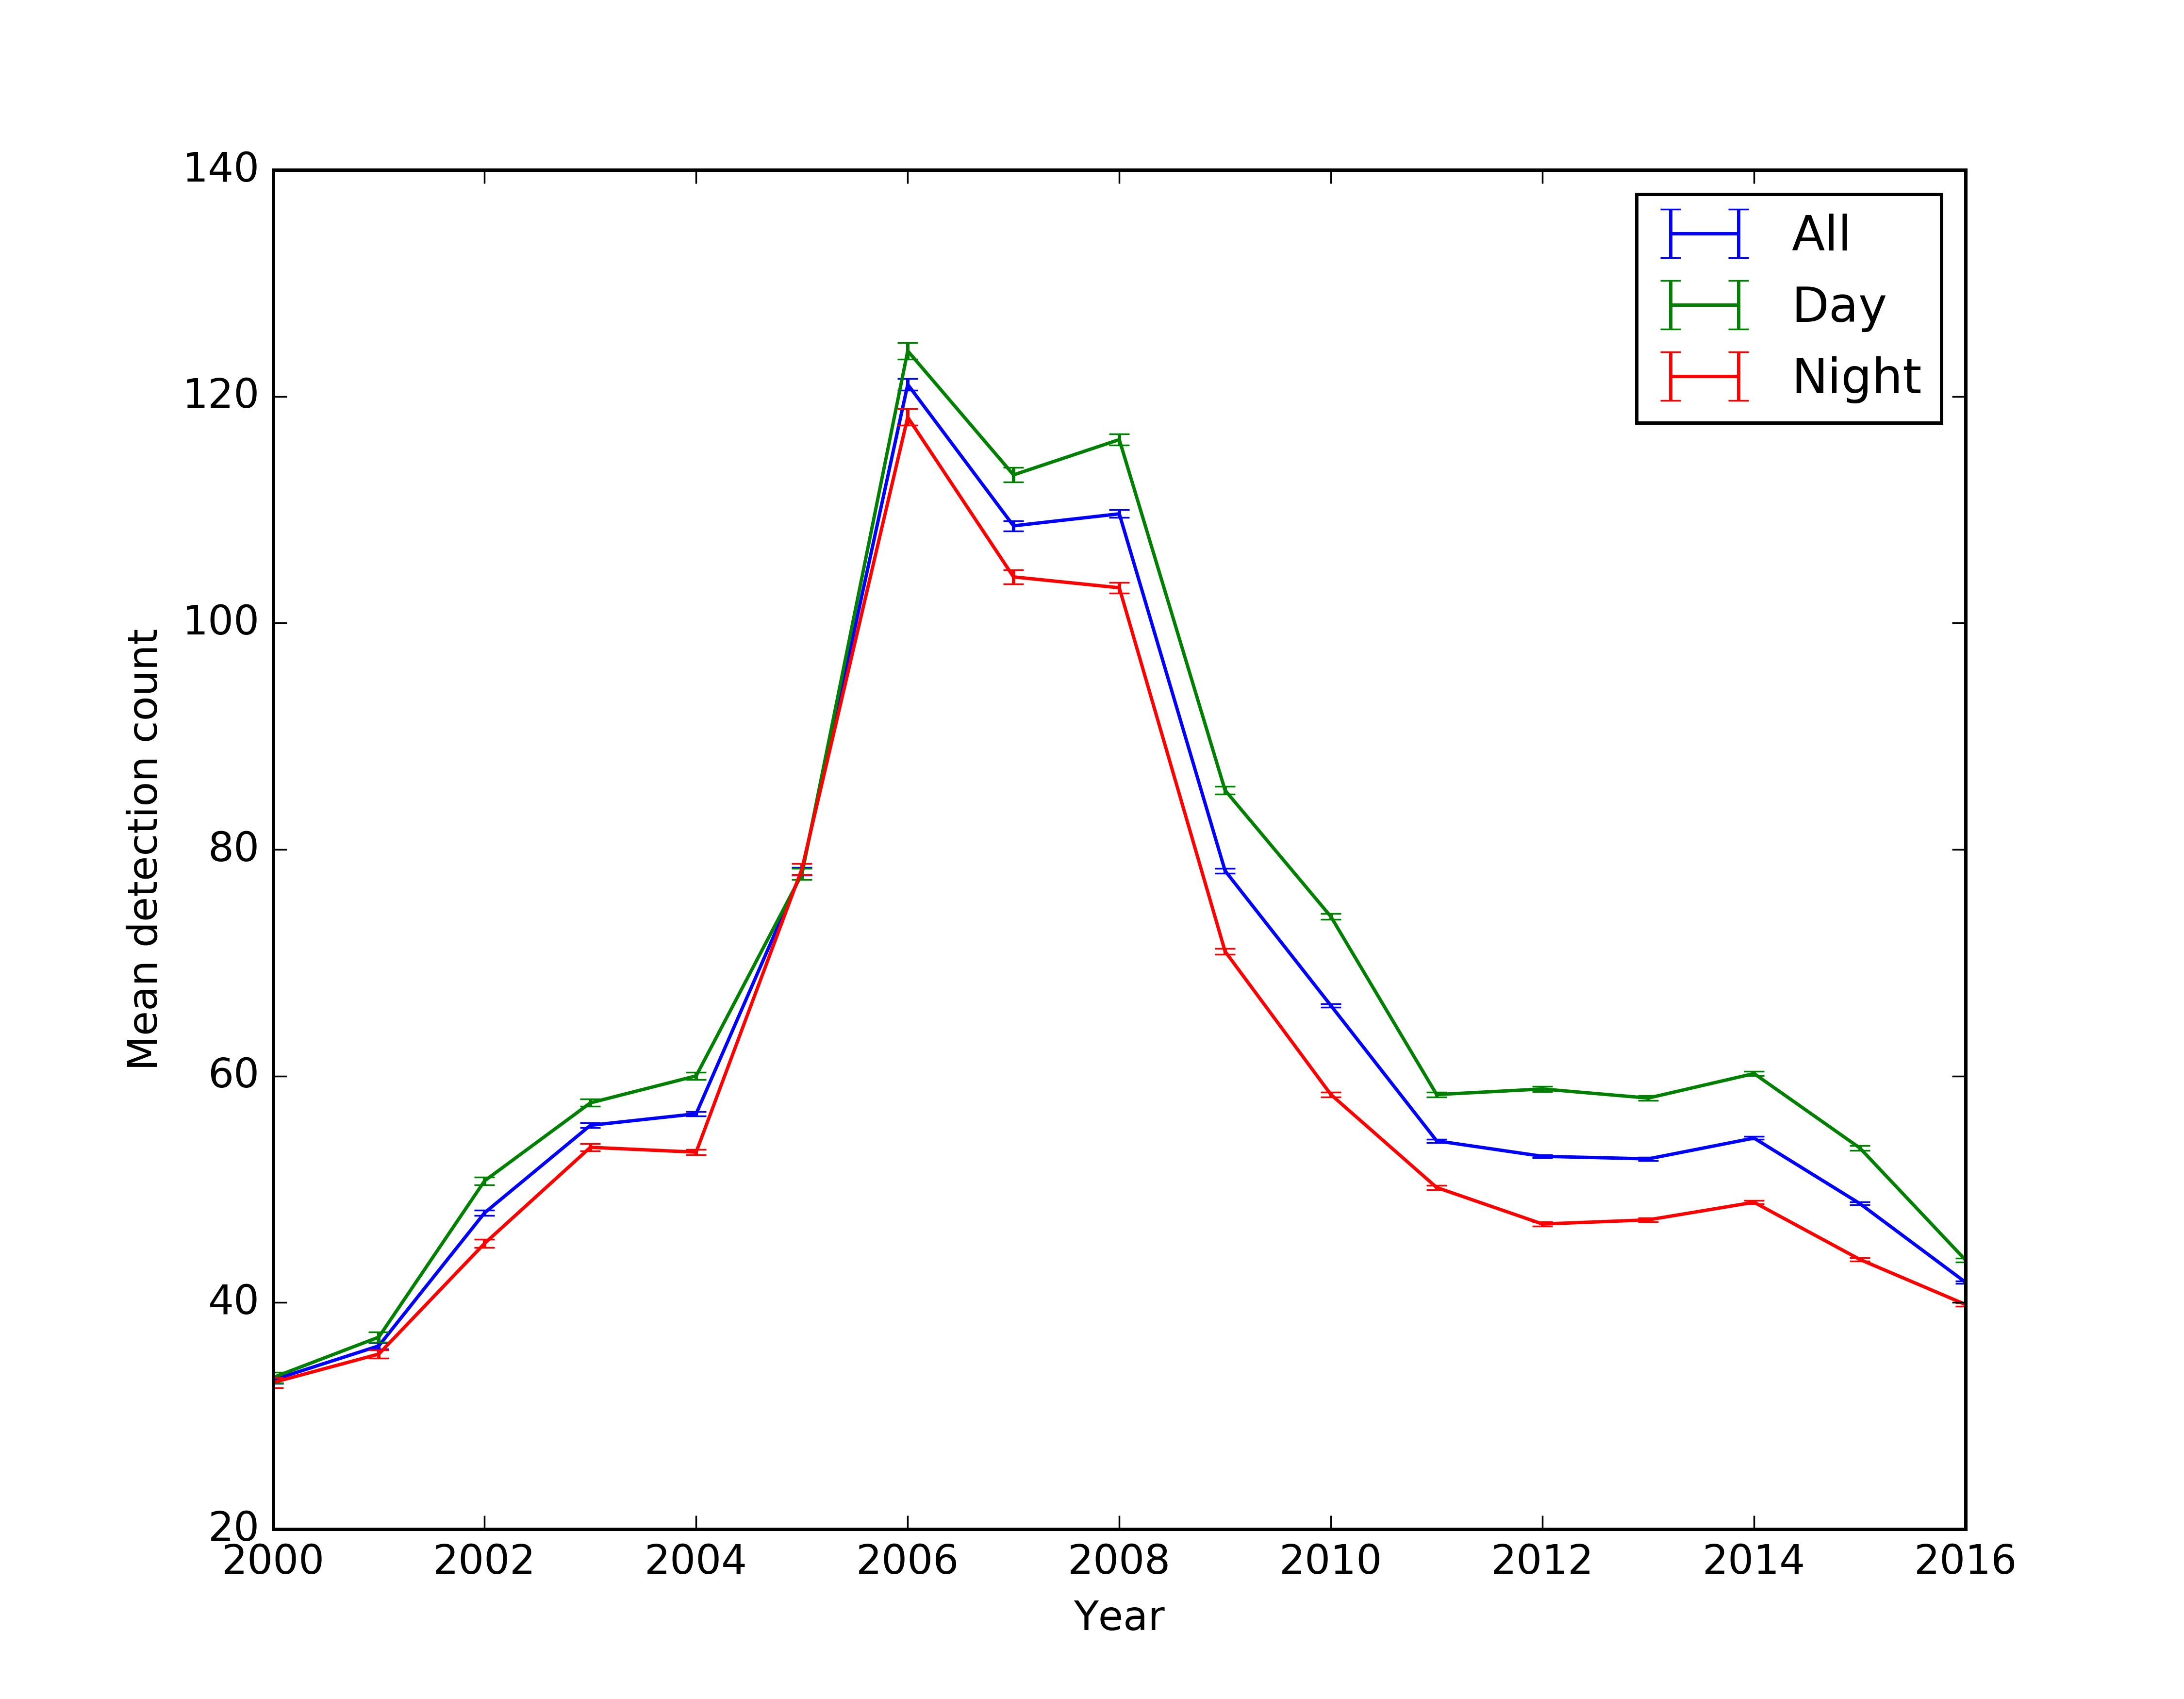
\includegraphics[width=\linewidth]{temporal/YAllcombined}
		\caption{All observers
			\label{fig:temp:daynight:a}}
	\end{subfigure}
	\hfill
	\begin{subfigure}[bh!]{0.475\textwidth}
		\centering
		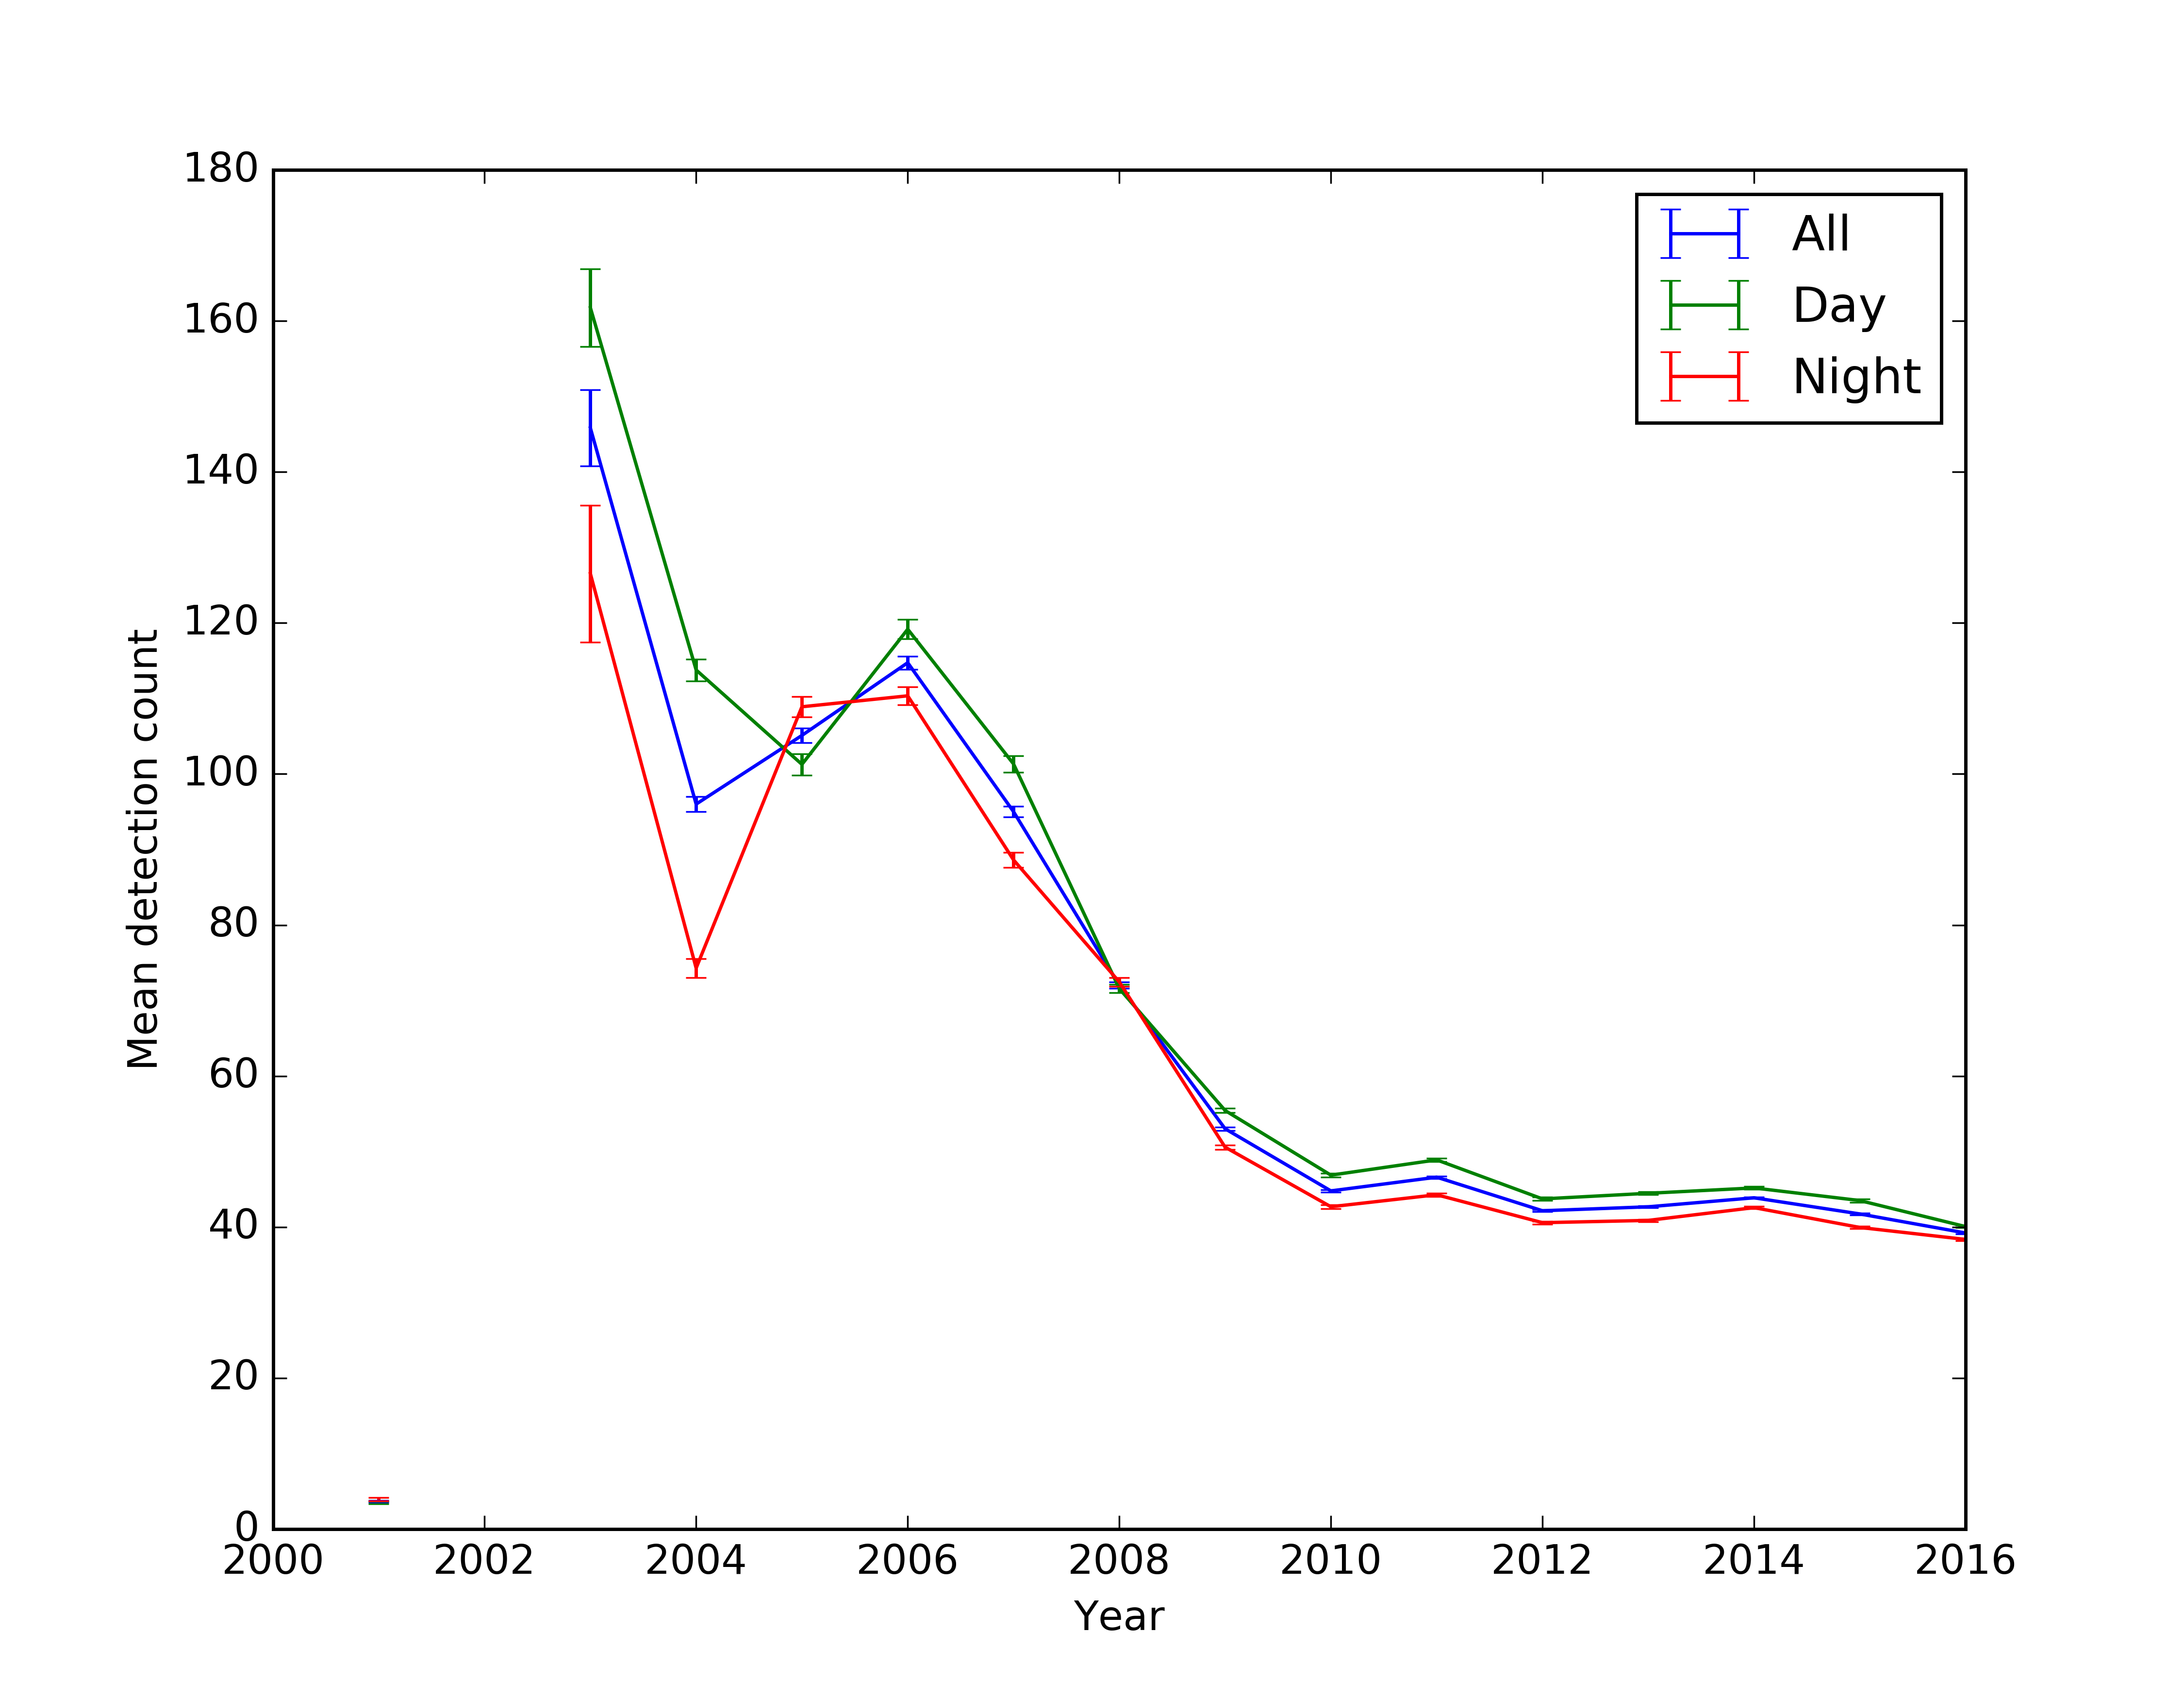
\includegraphics[width=\linewidth]{temporal/YEuropecombined}
		\caption{Observers in Europe
			\label{fig:temp:daynight:b}}
	\end{subfigure}
	\vskip\baselineskip
	\begin{subfigure}[bh!]{0.475\textwidth}
		\centering
		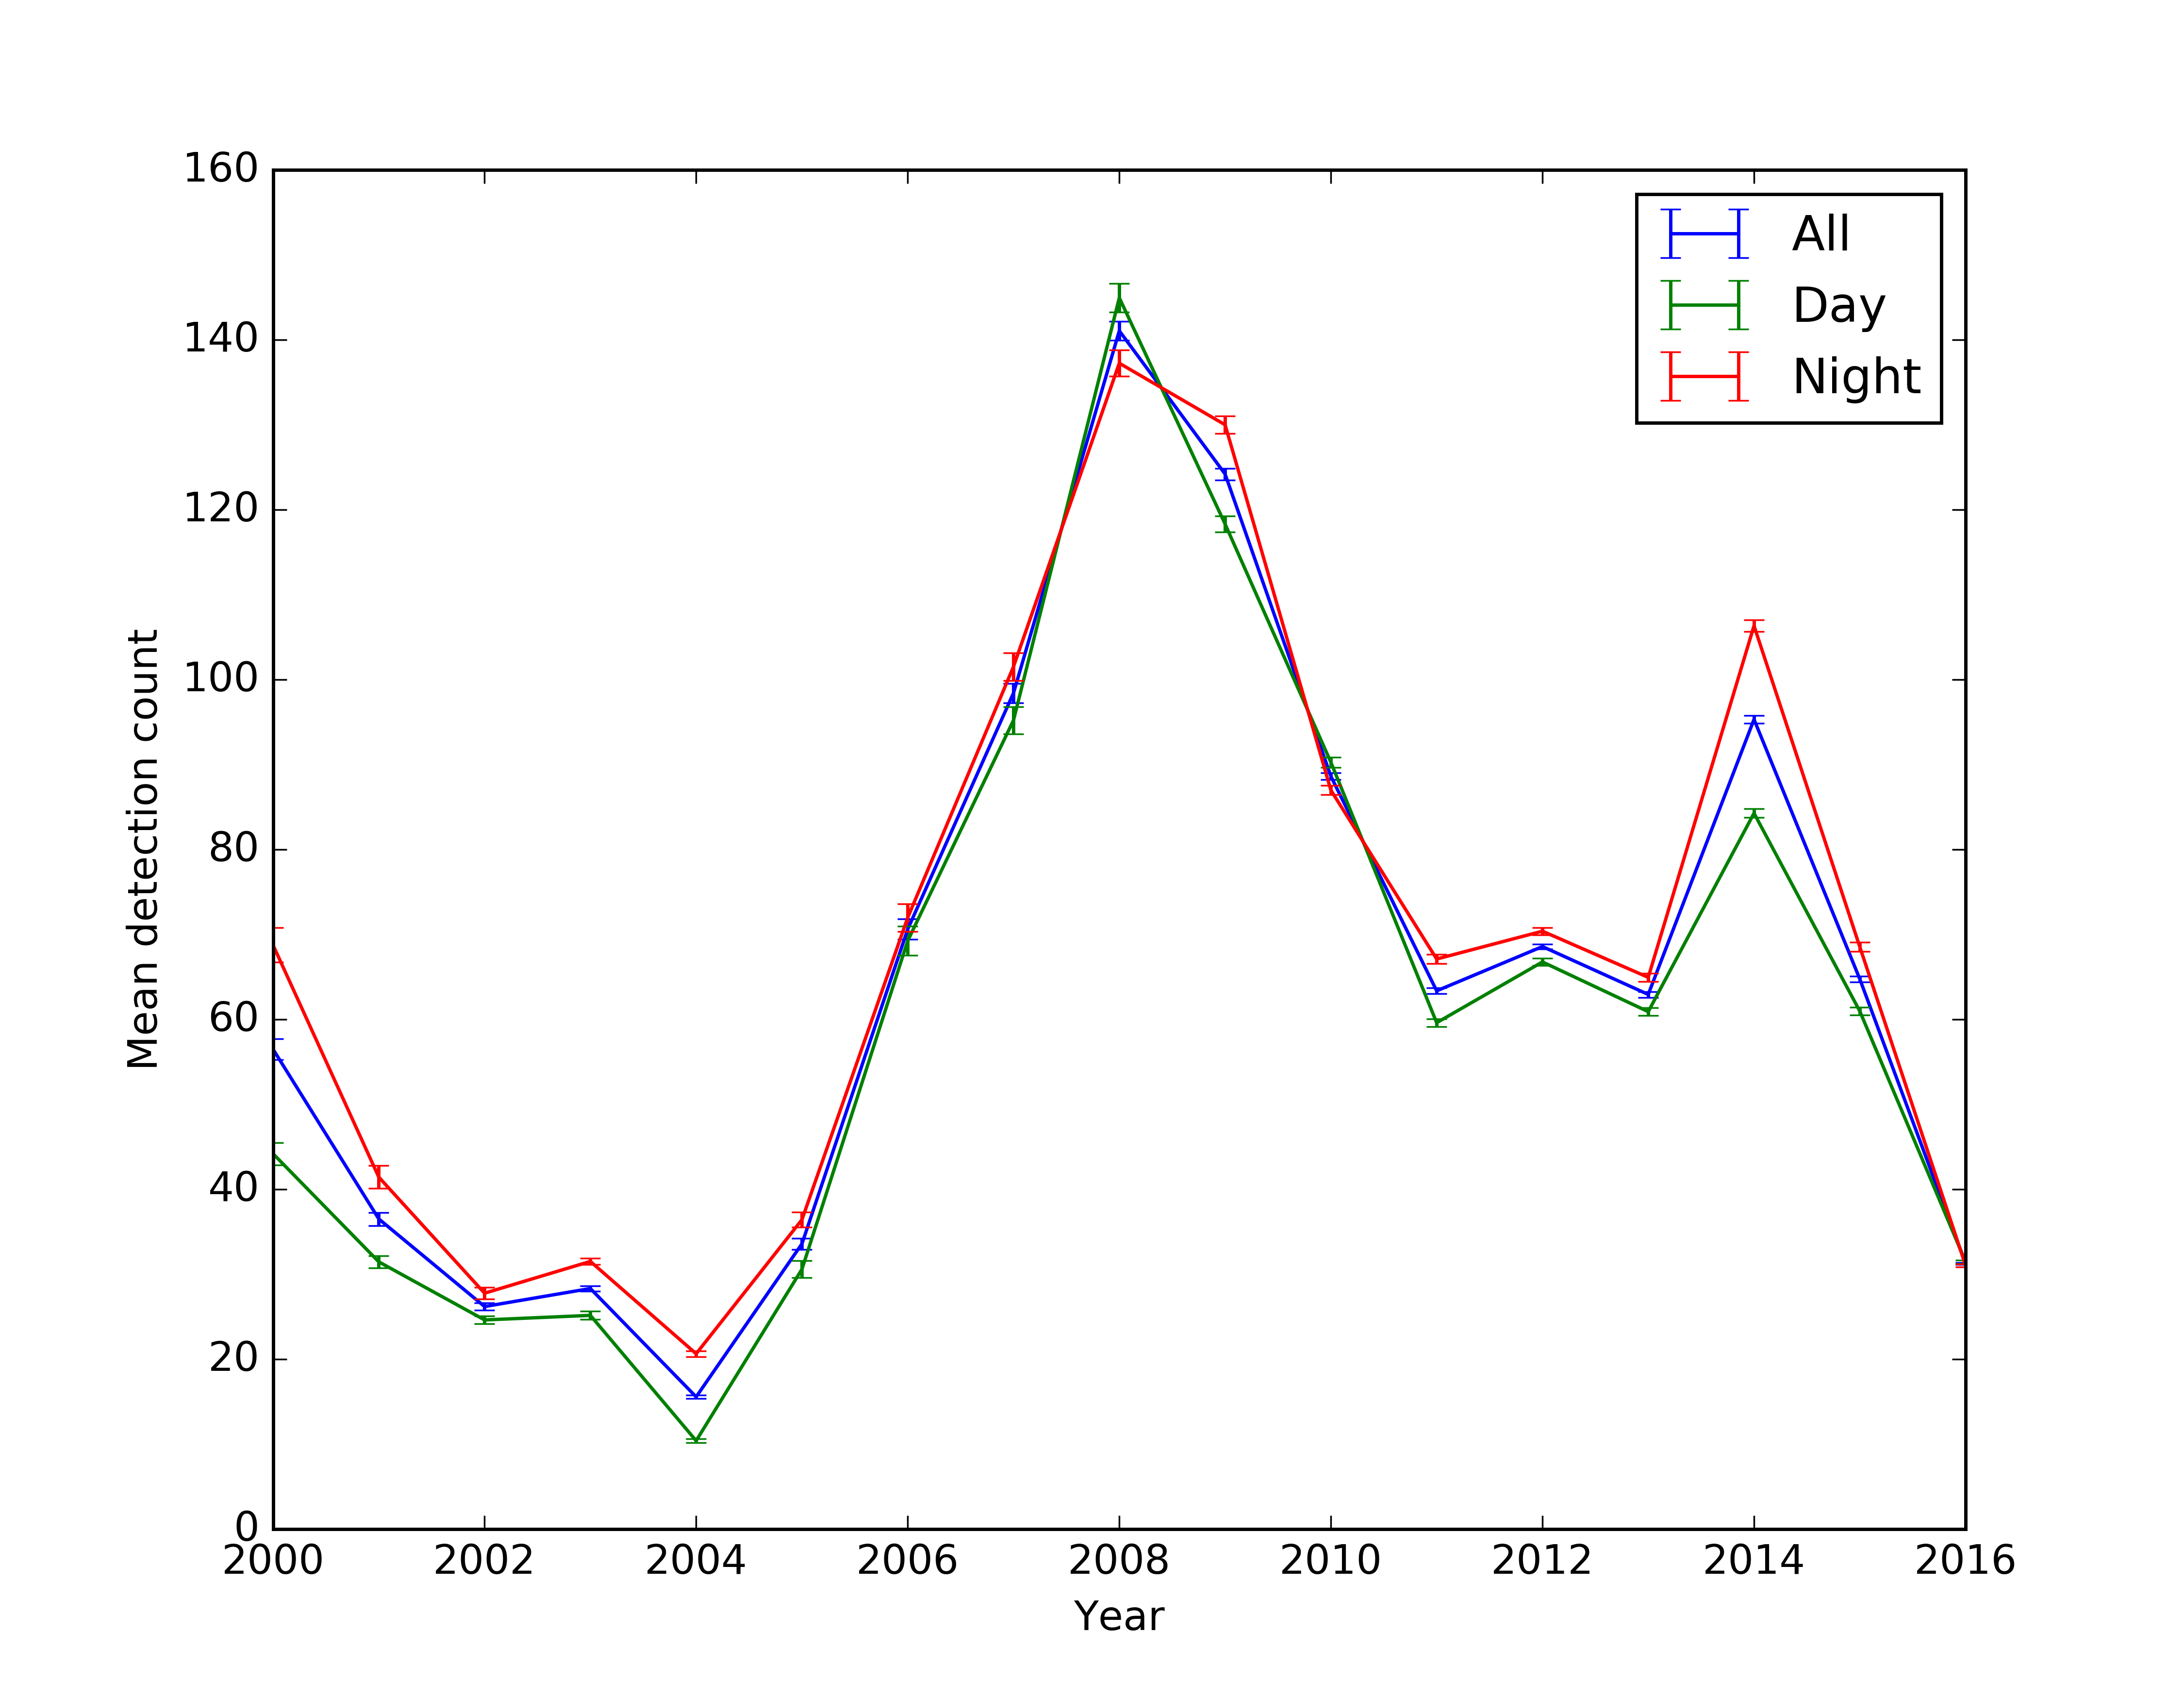
\includegraphics[width=\linewidth]{temporal/YnorthAmericaCombined}
		\caption{Observers in North America
			\label{fig:temp:daynight:c}}
	\end{subfigure}
	\quad
	\begin{subfigure}[bh!]{0.475\textwidth}
		\centering
		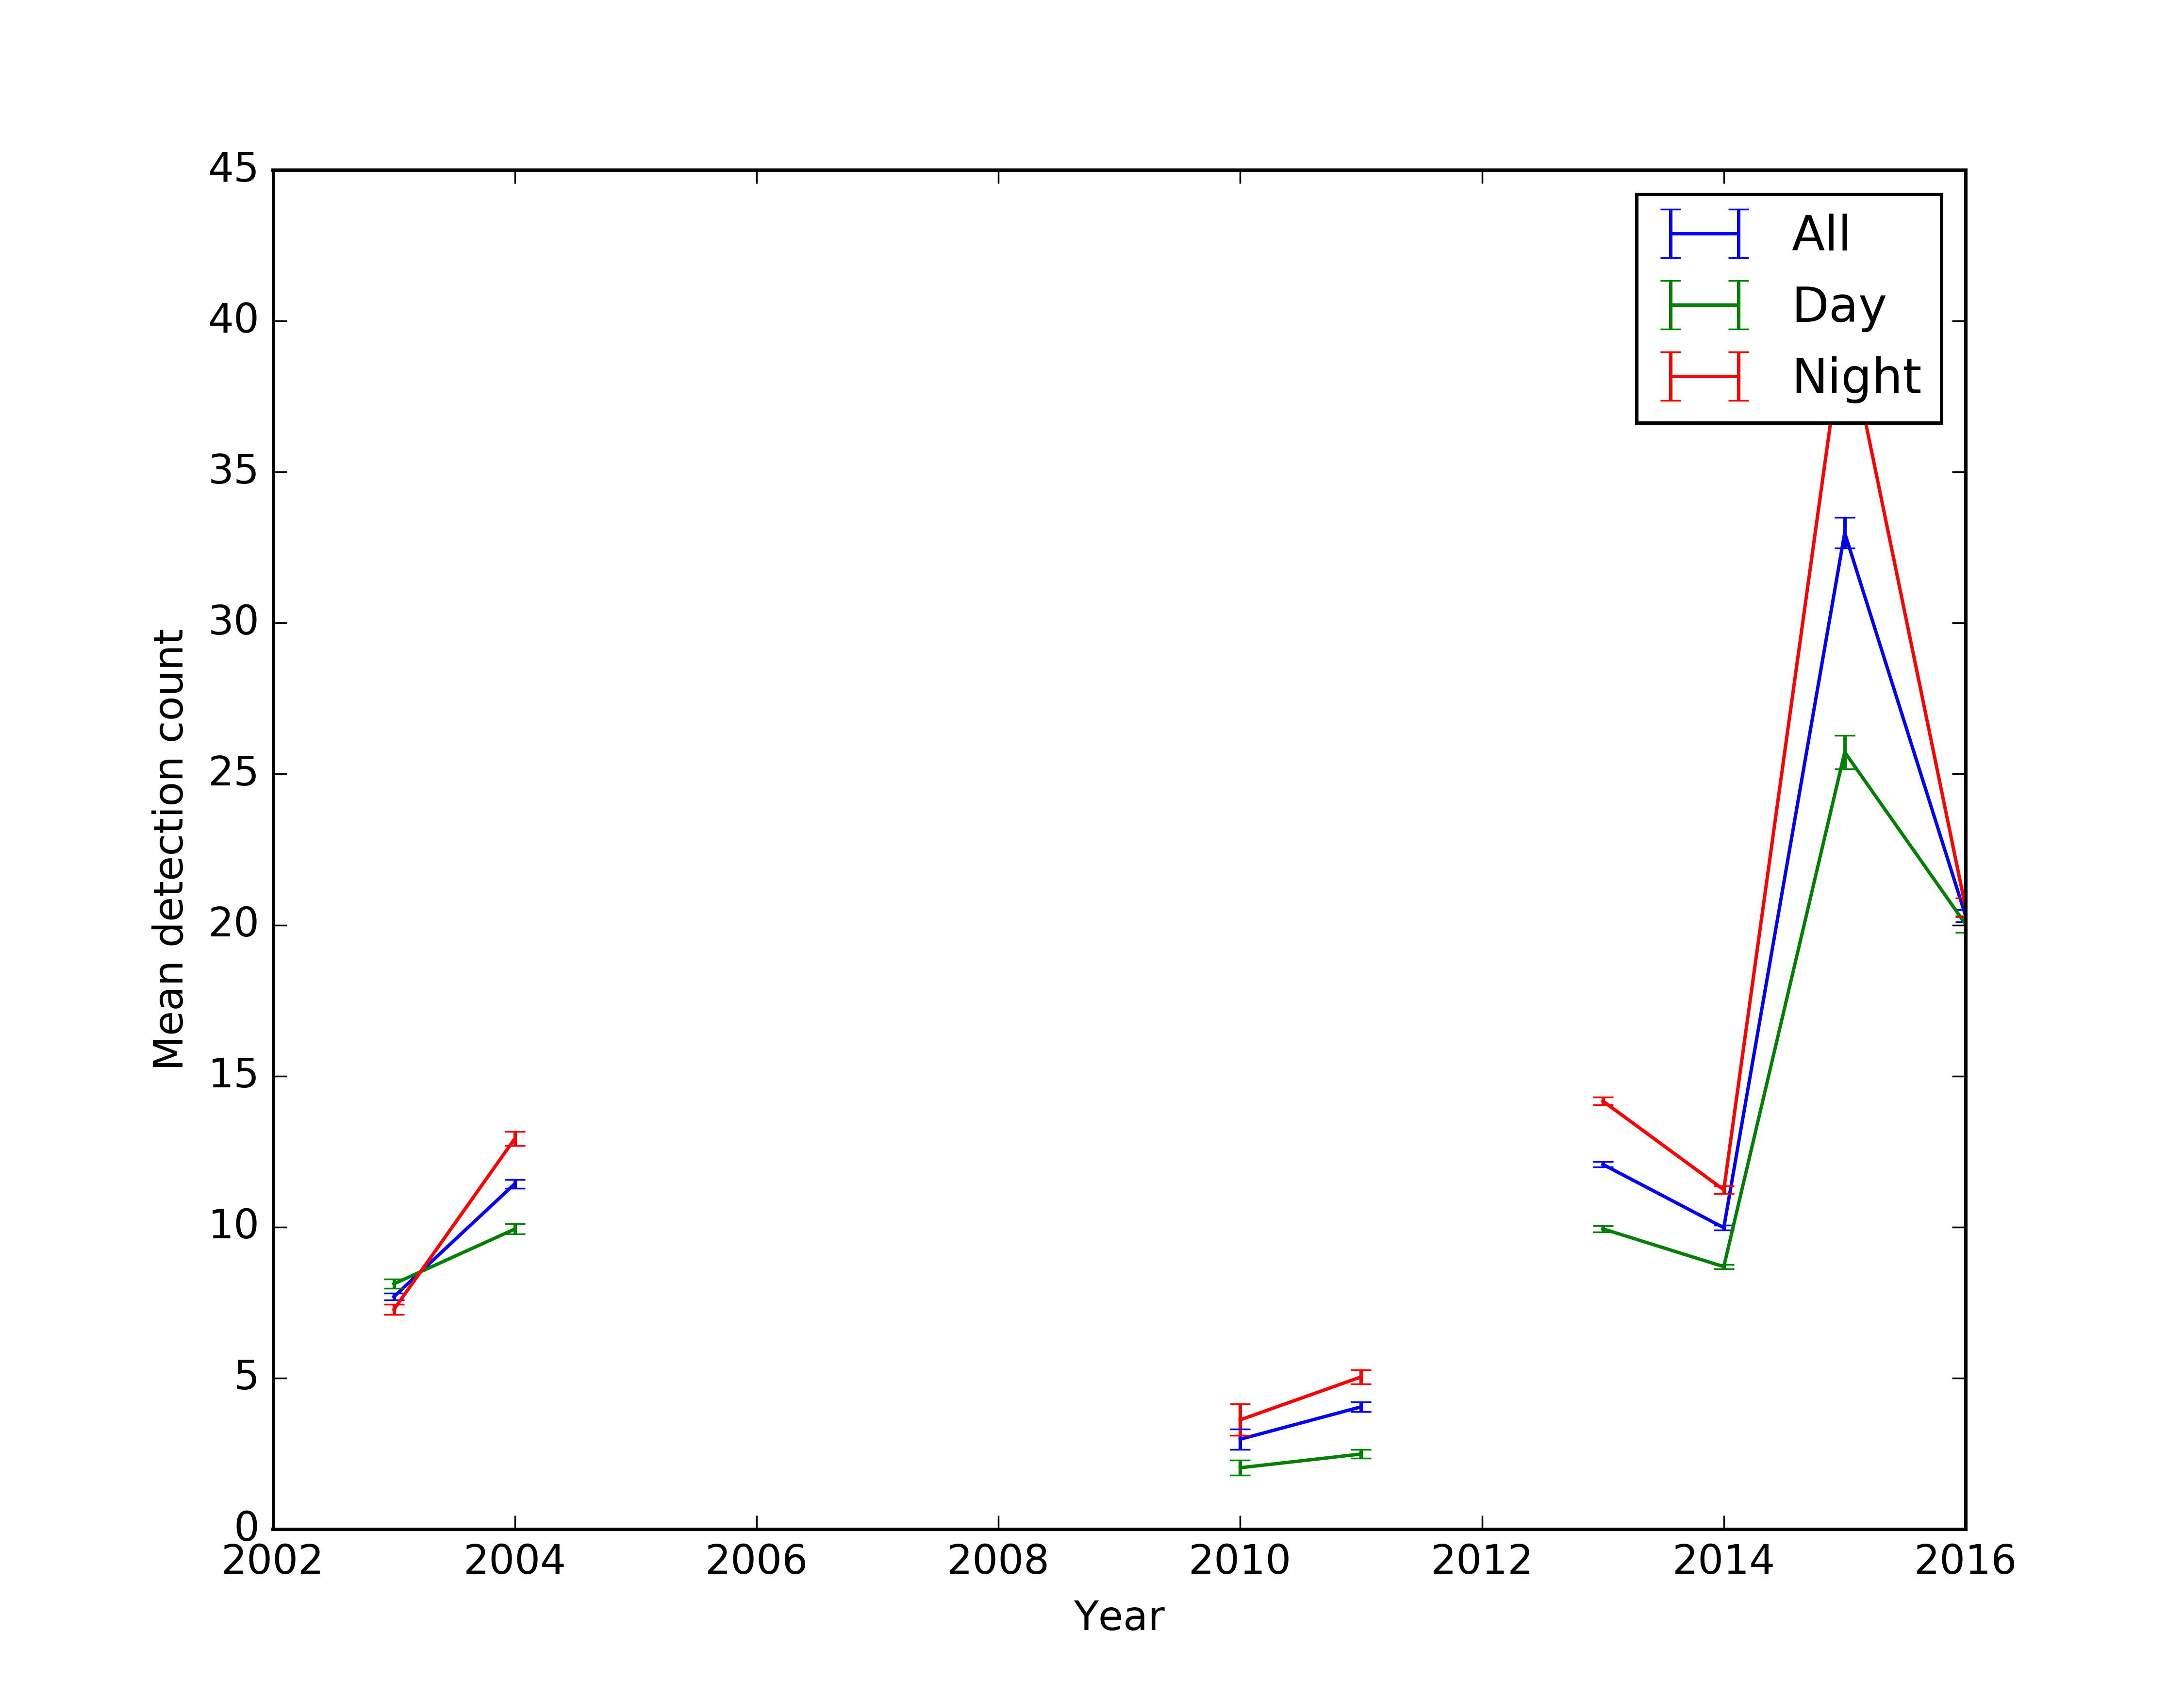
\includegraphics[width=\linewidth]{temporal/YasiaAustraliaCombined}
		\caption{Observers in Australia \& Asia
			\label{fig:temp:daynight:d}}
	\end{subfigure}
	\caption{Daytime vs. Night-time hourly detection counts}
\end{figure*}
\section{Discussion}
\subsection{Data characteristics}
\paragraph{Standard error\\}
The low variation shows that there are not large changes in hourly detection counts. This implies that influences from meteor showers do not greatly increase or decrease the detection counts, at least on a degree that would cause great variation. The increase from 2005 to 2011 agrees with figure~\ref{fig:temp:year}, where the variation greatly increases during the maximum in detection counts. The influence of a solar minimum, causing greater detection counts, supports this. With the absence of a strong solar wind, variations in the number of meteors are likely to have more effect.
\paragraph{Skewness\\}
It is expected that the skewness fluctuates around 0, primarily above 0. There will be an abrupt end in the distribution of possible detection counts since they cannot be negative, whereas there will be a tail towards large counts since there is (theoretically) no limit.
\paragraph{Diurnal shift\\}
I provide no explanation for the large amount of variation in the diurnal shift peak hour for earlier years, around 2000. In more recent years, the variation is less severe and the peak hour fluctuates around values that are expected from chapter~\ref{chap:diurnalshift}. There is a worse fit during the years where there is a maximum in detection counts, possibly because, with the greater detection counts, the diurnal shift has less influence on the total counts, meaning there is a worse fit for a sine function.
\subsection{Monthly scale variation}
It is expected that there is no overall trend over the course of a month. Any variation on this scale could potentially be caused by the moon, though it is unlikely that it would have an impact, and this is seen in the results. The small increase around the 11th-14th day of the month may be caused by a large shower, such as the Perseids, which causes such an increase in counts that it influences the mean across all months.
\subsection{Annual scale variation}
The increase in the middle of the year may be due to an increased number of meteor showers, or some other phenomenon. This increase can likely be considered part of the summer, since most observers in the sample are in the Northern Hemisphere. The low standard errors suggest that there is a clear periodic increase, and on the order of $\sim$ 20 counts an hour. The Asia \& Australia exhibits an increase, but two months earlier, and it does not persist for the rest of the year as other categories do. In chapter~\ref{chap:diurnalshift}, it appears from an analysis of fit between a sine-curve and a given observer's data that the background detection rate increases between 2005 and 2011. This result, and that presented in this chapter, appear to agree. I do not put forward any explanation for this increase; further investigation is required.
\begin{figure}[h!]
	\centering
	\includegraphics[width=\linewidth]{sunspots}
	\caption{Solar cycle sunspot number over time \cite{sunspot}
		\label{fig:temp:sunspot}}
\end{figure}
\subsection{Variation since 2000}
The increase centred around 2007 is significant. The maximum of the hourly detection counts occurs between 2006 and 2008, whilst the solar minimum occurs in 2009, however the sunspot number is not much larger than this from 2006, as can be seen in figure~\ref{fig:temp:sunspot}. This correlation (as well as a slight phase difference of 1 or 2 years) between solar minima and meteor maxima is noted in other articles \cite{lindblad}. That the solar cycle has an impact on meteor detection rates is not unexpected. The solar cycle influences heavily the solar wind and electron density, which will have a large influence on detection rates, especially for radio detection.
\paragraph{Daytime vs. night-time rates\\}
The fact that there is no significant difference between daytime and night-time counts seems to disagree with other studies. However, this simply rules out an influence from the Sun being above the horizon, or not. This does not discount the influence of the solar wind, since the change in electron density is not on only one side of the Earth. Thus any increase caused by the solar wind would not cause a significance difference between daytime and night-time counts. Theoretically, the peak hour of diurnal shift occurs at Sunset, so any influence will be uniform between day and night, so this can be disregarded.
\section{Conclusion}
I have found a significant increase in hourly detection counts between 2005 and 2011. The increase correlates well with solar activity, which supports hypothesis from Lindblad and Bumbda, as cited in section~\ref{sec:temp:litrev}. There is no basis to reject the hypothesis that the daytime and night-time hourly detection counts are different (1\% significance level), indicating that there is no influence on detection counts that varies over a single day's time frame. The results also show an increase in the middle of the year, which I provide no full explanation for. Further work on a hemispherical analysis may provide more information on this. A combination of a temporal and spacial analysis may also provide more information, since the two `dimensions' of variation often work in conjunction with one another.
\chapter{Antenna Data Characteristics}
\label{chap:antenna}
\begin{strip}
	\begin{minipage}{\textwidth}
		\begin{abstract}
			In this chapter I study the effect that antenna type has on the data produced by said antenna. This is done through an analysis of key characteristics describing important qualities of the data at hand. I find that, though there is variation between the differing types, there is no clear advantage for any of the considered antenna types. However, I also find that there are some indications as to which antenna type receives the best detection counts which may influence which antennas are used for future radio detection stations.
		\end{abstract}
	\end{minipage}
\end{strip}
\section{Background}
Radio meteor detection can use a variety of different antenna types. There are 12 main types used in the RMOB data I am using. Yagi antennas are overwhelmingly the most popular, followed by dipole antennas (see figure~\ref{fig:antennas}).
\begin{figure}[h!]
	\centering
	\includegraphics[width=\linewidth]{antennas}
	\caption{Antenna usage in RMOB data \label{fig:antennas}}
\end{figure}
Each antenna type has its own merits and cons, but that is a a discussion for another report. 
\section{Methodology}
\subsection{Selecting authors}
There are 12 antenna types that will be analysed. In order to carry out the analysis, the observers must be split into groups for each of these types. This was done through manual selection: displaying the antenna type of each observer (if it has one), and choosing which type this antenna is, through a Python program. Any unknown types were declared as miscellaneous. These categories were then saved to their own file.
\subsection{Analyses}
The analysis focused on 6 values, aimed at summarising and describing the detections made by the observers in each antenna category. Two of these values are the mean and maximum of all data collected by each respective observer. The minimum is of little importance, since the value will almost always be 0 or 1. These indicate the typical detection counts for the observer. The standard error of the same data set is also taken, which indicates how much the data varies. A lower value indicates that the same detection count is generally seen, and a larger value indicates that the detection count varies erratically. The skew also indicates the distribution of the detection counts. A positive skew indicates that the detection counts trail off towards high values, whilst a negative skew indicates that the distribution is `steeper' for higher values, suggesting that there is a limit to the detection counts. The last two values are the peak hour of the diurnal shift, and the fit to an optimised sine curve for the mean detection counts over each hour of a day. This is calculated by averaging the values for all data for a given hour after midnight. A sine curve is in then fit to this, in the same process as chapter~\ref{chap:diurnalshift}, giving a sine function of the form $N = A \sin \left( \omega t + \phi \right) + \mu$ where $N$ is the detection count and $t$ is the hour. The calculated `fit' is the sum of the standard deviations for $A$, $\mu$, and $\phi$. $\omega$ is assumed to be $\frac{2\pi}{24}$ so that the shift has a period of one day. A comparison is made of these 6 values for each antenna type.
\subsection{Sample sizes}
Sample sizes for each antenna category are shown below.
\begin{table}[h!]
	\begin{tabular}{cc}
		\hline
		Antenna & N$^o$ observers \\ \hline
		Diamond & 4 \\
		Discone & 12 \\
		Full wave loop & 5 \\
		Ground plane & 25 \\
		J-pole & 4 \\
		Log periodic & 6 \\
		Omni & 3 \\
		Quad & 3 \\
		Turnstile & 6 \\
		Vertical & 23 \\
		Yagi & 113 \\
		\hline
	\end{tabular}
\end{table}

\section{Results}
\subsection{Mean \& maximum}
Figure~\ref{fig:ant:meanmaxmin} shows the result for the mean and maximum counts for each hour, averaged for each respective antenna type. There is no clear difference between the means, as shown by the error bars, which show standard error. The largest mean is for a Turnstile antenna, though this is likely due to a single observer with a large detection count, and this is supported by the large standard error. There is also no significant difference in the maximum values. The most extreme (both large and small) maximum counts have larger error bars, which suggests that there are only a few observers which have these maximum counts out of all those in the antenna category.

\begin{figure}[h!]
	\centering
	\includegraphics[width=\linewidth]{antenna/meanmaxmin}
	\caption{Mean and maximum hourly detection counts (maximum count in red, mean in blue)
		\label{fig:ant:meanmaxmin}}
\end{figure}

\subsection{Standard error}
Figure~\ref{fig:ant:err} shows the results for the mean standard error of the hourly counts for each antenna category. The most extreme values have the largest error bars, suggesting that this is because there is a small sample size. However, the turnstile, vertical and j-pole antennas have the largest standard errors, suggesting these antennas produce data with the most variation. Log periodic, ground plane, full wave loop and diamond antennas have the 
lowest standard error suggesting the lower variation of the data.

\begin{figure}[h!]
	\centering
	\includegraphics[width=\linewidth]{antenna/err}
	\caption{Variation of hourly detection counts
		\label{fig:ant:err}}
\end{figure}

\subsection{Skew}
From figure~\ref{fig:ant:skew}, it can be seen that log periodic, vertical and Yagi antennas have the largest positive skew, with turnstile, discone and full wave loop antennas with the largest negative skew. Generally, a positive skew is expected since the data should trail off towards larger counts, whereas no counts are valid below 0, so there is a steeper end to the distribution of data. This is not seen in the data. The skewness values for each antenna category are relatively evenly distributed around 0. 5 of the categories have a standard error in the skew that is larger than the skew itself, suggesting that these values are not significant and cannot be considered completely valid.

\begin{figure}[h!]
	\centering
	\includegraphics[width=\linewidth]{antenna/skew}
	\caption{Skewness of hourly detection counts
		\label{fig:ant:skew}}
\end{figure}

\subsection{Diurnal shift}
The results are relatively evenly distributed around a peak hour of 9: however, as found in chapter~\ref{chap:spatial}, this is most likely due to the geographical location where the antenna is used. Based on this, it is likely that ground plane, omni, quad and turnstile antennas are mostly used in Europe, whilst full wave loop, J-pole and diamond antennas are used mostly at latitudes ${\sim} -180^{\circ}$ and $180^{\circ}$.

\begin{figure}[h!]
	\centering
	\includegraphics[width=\linewidth]{antenna/peak}
	\caption{Peak hour of diurnal shift
		\label{fig:ant:peak}}
\end{figure}

The larger results for J-pole, quad, turnstile and vertical antennas suggests that these are not as influenced by diurnal shift. However, these categories have much larger standard errors than other categories, suggesting that there is simply a low sample size. Vice versa, ground plane and log periodic antennas have much better fits to a sine curve, implying the antennas are more influenced by diurnal shift.
\begin{figure}[h!]
	\centering
	\includegraphics[width=\linewidth]{antenna/fit}
	\caption{Fit to optimal sine function for diurnal shift
		\label{fig:ant:fit}}
\end{figure}

\section{Discussion}
\subsection{Mean \& maximum}
There is no clear trend for an antenna which produces data which, on average, has greater hourly counts. This is expected. Were there an antenna that was particularly good at radio meteor detection, it would likely be used widely. Equally, if there was an antenna that produced particularly poor data, it would not be used at all. The standard errors, for all categories, range across ${\sim}$ 20 counts an hour. This is substantial, and suggests that there is little agreement between characteristics of data for observers that use the same antennas.
\subsection{Standard error}
For some categories, the mean standard error is much larger. However, these categories have greater errors. Diamond, full wave loop, ground plane, and log periodic antennas appear to produce data with the lowest amount of variation. The implication is that the antennas are poor at detection meteors, so there will be little variation in the counts. However, comparing these categories with figure~\ref{fig:ant:meanmaxmin}, they are the lowest categories (other than full wave loop), but not significantly lower than others. 
\subsection{Skew}
Log periodic, vertical and Yagi antennas all appear to produce reasonably positively skewed data. The same extremity is not seen for a negative skew. Other than vertical antennas, the error is not too large, indicating that there is {\it some} correlation. A lack of correlation with other properties indicates that this is an anomalous result. However, further investigation may yield this to be false.
\subsection{Diurnal shift}
Variations in the peak hour of diurnal shift are likely due to location, as discussed in chapter~\ref{chap:diurnalshift} and \ref{chap:spatial}. However, most antennas appear to produce data with peaks around hour ${\sim}$ 9. Errors for all categories are substantial, indicating little agreement within each category. Ground plane and log periodic antennas appear to produce data that fits a sine-function very well, indicating a greater periodicity in the data than other antennas. The poorest fits have large standard errors, indicating that these values are of little validity.
\subsection{Improvements}
\paragraph{Location}
From previous chapters, it is known that the location where data is collected will influence the results. Because of this, simply grouping together observers who use the same antenna may not give an accurate reflection of the data characteristics unless the data is somehow normalised so that location has no effect. The simplest way to do this is to include more observers, and then analyse the antenna categories. When comparing these results, the location can be factored into any conclusions, removing the influence that location has on the data.
\paragraph{Yagi n-element analysis\\}
In my analysis I have grouped {\it all} Yagi antennas into the same category. An analysis based on the number of elements on the antenna within the yagi category may indicate if there is an optimal number of elements for meteor detection, as well as the effect of different numbers of elements on the characteristics of the data.
\paragraph{Coefficient of variation\\} 
Instead of using standard error of the hourly detection counts to indicate the variation of the data, it may be better to use the coefficient of variation, $c_v$, defined as $c_v = \frac{\sigma}{\mu}$ where $\mu$ and $\sigma$ are the mean and standard deviation of the data respectively. This gives a better reflection of the variation as instead of factoring in the sample size, it factors in the mean. This is an improvement since the degree of variation is no longer proportional to the mean, giving no skew favouring lower means.
\paragraph{Percentiles\\}
As part of the data characteristics analysis, I used the maximum count to help summarise the data. This is not a very useful summary value to make, since the maximum itself holds little value. What would indicate the distribution of data better is a value such as the 90th percentile. This may give a better reflection of the data that an antenna produces.
\section{Conclusion}
There is no clear correlation between any characteristics and the antenna types. However, J-pole, log periodic and turnstile antennas consistently have the most extreme values. However, the extremes for these antenna types do not necessarily imply the same characteristics of the data. Log periodic antennas appear to provide consistently positive-skewed data. Turnstile antennas appear to provide the largest detection counts. A consistent theme throughout the results are large errors, suggesting large variation within each antenna category, implying little correlation between the given antenna type and the characteristic under consideration. Greater sample sizes, as well as isolation of other variables (location, time) may reveal more correlation.
\chapter{Zenithal Hourly Rate Validity for Radio Detection}
\label{chap:zhr}
\begin{strip}
	\begin{minipage}{\textwidth}
		\begin{abstract}
			I present an improved formula for calculating Zenithal Hourly Rate (ZHR) and an analysis of its validity for radio meteor detection. Beyond this, I assess the implications of the resultant ZHRs for antenna field of view, meteor shower population index and stream density. The formula, with modification is valid, and the results agree well with visual results. There are clear improvements that can be made, though as a first approximation the formula is adequate.
		\end{abstract}
		\keywords{meteors, radio meteor detection, zenithal hourly rate, population index, radiant, meteor shower}
	\end{minipage}
\end{strip}
\section{Background}
Zenithal Hourly Rate (ZHR) is a measure of the activity of a meteor shower. The value indicates how many meteors an observer can expect to see, assuming optimal viewing conditions, with the meteor shower's radiant at the observer's zenith (directly overhead).
\section{Literature Review}
\subsection{Calculating ZHR}
A formula already exists for calculating the theoretical ZHR from known data and conditions \cite{zhr}. The formula (\ref{eq:zhr}) depends on four correction factors.
\begin{equation}{ZHR} = \frac{\overline{HR} \cdot F \cdot r^{6.5-{m}}}{\sin \left( h \right)}\label{eq:zhr} \end{equation}
The hourly rate is given by $\overline{HR} = \frac{N}{T_{eff}}$, $N$ is the number of meteors observed, and $T_{eff}$ is the effective observation time of the observer. This corrects the number of meteors detected such that it is an hourly rate. \\
The correction for the field of view, $F$, is given by $\frac{1}{1-k}$ where k is the percentage of the observer's field of view that is obstructed. \\
The correction factor for limiting magnitude is given by $r^{6.5-m}$, where $m$ is the limiting magnitude of the observer. This corrects the value such that it is representative of the ZHR when the limiting magnitude is 6.5.  The value of $r$ itself is the population index; a measure of the magnitude distribution of the shower. For each increase by 1 in magnitude (bearing in mind that a greater magnitude is a lower value), the number of meteors you would expect to see increases by $r$.\\
The final correction factor is for the altitude of the radiant above the horizon, measured as an angle. This is effectively $\frac{\pi}{2}-z$ where z is the zenith distance in radians. The radiant is the observed point of origin for all meteors in the shower. This correction factor is given by $\sin h$ where $h$ is the angle from the horizon to the radiant.\\
\subsection{Meteor shower information}
The International Meteor Organisation (IMO) provides a list of ``meteor shower calendars'' \cite{imo_meteor_calendar}. These contain a list of notable meteor showers, with information on these showers including the active range (period in which the shower produces visible meteors), the date of it's maximum, the expected ZHR, radiant co-ordinates (in right ascension and declination), and finally the population index. This calendar will be the source of my data for visual observation data, and will provide the information from which comparisons can be made with the radio observation data.
\section{Methodology}
\subsection{Assumptions}
The following assumptions are made in my calculations.
\begin{itemize}
	\item The receiving antenna is active for the entire period where data is available.
	\item The antenna detects meteors across the entire sky.
	\item Detected meteors are travelling tangential to Earth's surface.
	\item The shower meteors are incident uniformly in all directions around the radiant.
\end{itemize}
\subsection{Formula modification}
The formula \cite{zhr} for ZHR has a number of issues that cause inaccurate results. In order to use the formula in my analysis, these errors must be corrected.
\subsubsection{Inaccuracy of radiant height correction}
\paragraph{Problems\\}
Perhaps the largest error is that of the radiant height correction. The correction assumes a sine function of the angular radiant height, which varies (with $-\pi \leq h \leq \pi$) between -1 (for $h = -\pi$) and 1 (for $h = \pi$). This creates a number of issues: when the radiant approaches the horizon, $h$ approaches 0, as does $\sin h$. This means that the correction (which is $\frac{1}{\sin h}$) approaches $\inf$. This is clearly wrong. When the radiant approaches the horizon, the number of meteors observed doesn't approach 0, and thus the correction should not approach $\inf$. In other words, you do not see infinitely many meteors when the radiant is at the zenith compared to the horizon. Further to this, the use of a sine function simply means that there is \textit{no} way a calculation can be made when the radiant is at the horizon --- this should be possible. The sine function also results in a negative ZHR when the radiant is below the horizon. Clearly, you do not expect to see anti-meteors when the radiant is below the horizon. 

\paragraph{Previous Solution}
Solutions to the issue with the radiant height correction factor have been studied previously \cite{hr_correction}. In this article, a piecewise function is noted from Kres\'{a}k \cite{kresak} which uses a cosine function of the zenith distance (which equates to a sine function of the radiant altitude) down to 80$^{\circ}$, and then uses another function which extends the domain of the model to $\sim$100$^{\circ}$. The article itself puts forward a complex function which works over a similar domain. This is not a first approximation though, it is an attempt at an accurate function to describe the flux correction factor for a range of radiant altitudes. The article notes that there is a small, yet present, possibility of shower meteors for a radiant below the horizon, and the reason for this dramatically lower expected detection count is that the atmosphere shields the Earth from most of the debris, and only those travelling tangential to the Earth's surface are detected. This may be applicable to visual observation, but radio detection almost relies on meteors travelling tangential to the Earth's surface, so the radiant being below the horizon does not have such a dramatic effect. For this reason, I do not believe this is a useful replacement for the correction factor.

\paragraph{Solution\\}
From a basic geometric standpoint, the number of meteors you expect to observe, varying with the radiant height, should depend on the proportion of a hemisphere (with the radiant at the pole) that is visible. Of course, this assumes that meteors travel from the radiant uniformly in all directions. 
\begin{figure}[h!]
	\centering
	\includestandalone[mode=buildnew, width=\linewidth]{wedge}
	\caption{Spherical wedge curved surface area \label{fig:wedge}}
\end{figure}
A wedge of a sphere has a curved surface area of $2{\alpha}r^2$, where $\alpha$ is the angle at the central axis of the wedge (see figure~\ref{fig:wedge}). Thus, the proportion, $p$, of the hemisphere that is visible is $\frac{2{\alpha}r^2}{2{\pi}r^2} = \frac{\alpha}{\pi}$. For an angle $h$ (the radiant height as an angular distance) varying between $-\frac{\pi}{2}$ and $\frac{\pi}{2}$, the proportion will vary between -1 and 1 (perhaps where the original sine factor came from). When the radiant is at the zenith, you would obviously expect to see the same number as if the radiant was at the zenith, so the correction factor, $c$, is 1 (see figure~\ref{fig:hemisphere}). 
\begin{figure}[h!]
	\centering
	\includestandalone[mode=buildnew, width=\linewidth]{diagram}
	\caption{Diagram for derivation of radiant height correction factor. The shaded hemisphere is the observer's field of view. \label{fig:hemisphere}}
\end{figure}
When the radiant is at the horizon, half the hemisphere is visible, so you would expect to see half the number of meteors at the zenith ($c = 2$), and when the radiant is directly below you (at the nadir) then you would expect to see no meteors (from the shower), since none of the hemisphere of the radiant is visible to you. Mapping the proportion linearly from $-1 < p \leq 1$ to $0 < \frac{1}{c} \leq 1$ yields $\frac{1}{c} = \frac{1}{2} + \frac{h}{\pi}$ for $-\frac{\pi}{2} < h \leq \frac{\pi}{2}$, where $h$ is in radians. This satisfies the \textit{expected} correction factor.

\subsubsection{Population index limitations}
The population index indicates the magnitude distribution of the meteor shower. For each extra magnitude of visibility, an observer would expect to see $r$ times more meteors. This is true, but only up to a point. Without a limit on how far this model works, the implication is that this power-law distribution carries on forever. Clearly this is not true: if limiting magnitude was (rather absurdly) 40, you wouldn't expect to see 1.1 trillion meteors (if $r=2.0$). Thus the model is not applicable for limiting magnitude, $m > 6.5$, since the model that the magnitude distribution is of the form $N = N_or^m$ is no longer valid. The radio observation of meteors has a larger limiting magnitude than visual observation: meteors down to the size of a grain of sand, and smaller, can be detected. Thus the population index model is not applicable for radio meteor detection, unless the model is refined for larger limiting magnitudes.

\subsubsection{Background detection count}
In visual observation of meteors, the background level of sporadic meteors is rather low. However, for radio meteor detection, there is a much greater background detection rate and this will impact how accurate the ZHR is. A correction is required to remove the effect of any background detection rates. The calculation of this background rate is a chapter in itself. The difficulty arises in that if the baseline is larger than any detection counts within the active range, the resulting ZHR will be negative, and this is not a valid result. A solution to this is to choose the minimum hourly detection count in the active range of the shower, but this is rather artificial, and often results in a baseline of 1 or 0. Instead, I have decided to calculate the background hourly detection count by taking the mean hourly detection count for the lower quartile of all hours outside the active range of any meteor showers. This will result in some ZHRs being negative, but these results should be minimal and can simply be discarded.
\subsubsection{Field of view correction}
I will not include a field of view correction factor, since it is not possible to know exactly the field of view that each antenna has available, since it is not part of any data that an observer can upload to RMOB. This \textit{should} have a reasonably large impact on the results, however the correction factor will be absent for all calculations so the error is the same everywhere (on average). In fact, using the final results may allow the average field of view to be calculated.
\subsection{Calculating radiant height}
From the spherical law of cosines, we know that 
\[ \cos z =  \sin \phi \sin \delta + \cos \phi \cos \delta \cos \left(\theta - \alpha\right)\]
where $z$ is the zenith distance, $\phi$ is the observer's latitude, $\alpha$ and $\delta$ are the right ascension and declination of the shower radiant, and $\theta$ is the local apparent hour angle (an angular measure of local sidereal time, which effectively measures time against the stars rather than the Earth's rotation). Since $h = \frac{\pi}{2} - z$, $\cos z$ can be replaced with $\sin h$. This relations the radiant altitude to the longitude of the observer and the radiants astronomical co-ordinates.
\subsection{Calculating hourly rate}
The hourly rate is given by the observed hourly rate (the data I actually have), minus the baseline hourly rate. This \textit{should} be divided by the effective observation time, but since I am making the assumption that the antenna are receiving across the entire hour, then there is no need for this.
\subsection{Analysis}
\paragraph{Selecting observers}
In order to carry out the analyses, the observers had to be split into groups for each shower. This was done simply by checking which months each observer was active for, and adding it to a given category if the observer is active during the shower. This selection was refined further so that an observer must be active for the entire peak date, and have no more than 12 inactive hours during the active period of the shower. The sample sizes for each shower are shown in table~\ref{tab:zhr:sizes}.
\begin{table}
	\centering
	\begin{tabular}{cc}
		\hline
		Shower & N$^{\circ}$ observers \\
		\hline
		Geminids & 67 \\
		Leonids & 61 \\
		Orionids & 43 \\
		Perseids & 39 \\
		Quadrantids & 58 \\
		$\eta$ aquariids & 34 \\
		\hline
	\end{tabular}
	\caption{Sample sizes for meteor showers
		\label{tab:zhr:sizes}}
\end{table}
\paragraph{Comparison\\}
My analysis of the ZHR will centre around a comparison between the summary statistics for the ZHRs from the hourly counts for the stored observers, and known values for the ZHRs for applicable years. The process of calculating the ZHR follows a simple process of calculating the correction factors, correcting the known hourly rate, and discarding any invalid values (e.g. negatives). The formula, after modification, is
\[ {ZHR} = \frac{N - r}{\left( \frac{1}{2} + \frac{h}{2\pi} \right)} \]
where $r$ is the background hourly rate, and $N$ is the number of meteors detected for one hour. The error is given by
\[ {S.E.} = \frac{{ZHR}}{\sqrt{N}}\]
This calculation will be done for each hour available, and then a mean will be taken. This process will be applied to three ranges of dates: the entire active period of the shower (for a given year), two days either side of the peak date, and the peak date. Once this has been calculated for all the available data in the given ranges, the mean and 90th percentile are recorded. These will then be compared to the known values from the IMO meteor shower calendar \cite{imo_meteor_calendar}. I am using the 90th percentile rather than the maximum ZHR since the maximum itself is of little worth to indicate the distribution of ZHRs. A box plot for each year of each shower would yield the most information but would provide far too much data to consider at once, whereas the 90th percentile indicates the maximum clearly without producing the exact same result if, for instance, the maximum ZHR was the same across all three periods under consideration. 
\paragraph{Correction factors\\}
The final results will then be used to estimate the average field of view across all observers whose data are used, as well as the average limiting magnitude. This is a rough calculation, and is likely to have a large uncertainty, but it gives an estimate towards the true values and is an interesting calculation to make. The formula for the field of view factor is
\[ k = 1 - \frac{{ZHR}_{mean}}{{ZHR}_{exp}} \]
For the limiting magnitude,
\[ m =  \log_r \frac{r^{6.5} \cdot {ZHR}_{mean}}{{ZHR}_{exp}} \]
For each of these calculations, $ZHR_{mean}$ is the calculated mean ZHR for the peak of the shower, and $ZHR_{exp}$ is the maximum visual ZHR for the same shower and year.
It is clear that a negative $k$ will be the result when the mean ZHR of the peak is less than expected, and positive otherwise. Any negative values can be discarded. Equally, a limiting magnitude will be less than 6.5 if the mean ZHR of the peak is less than expected, otherwise it will be larger than 6.5. Values less than 6.5 can be discarded. This means that the correction factor that applies will either be for field of view, or limiting magnitude, not both.
\section{Results}
The full results are shown in appendix~\ref{app:zhr}. In this section, important results are noted.
\subsection{Comparison}
\paragraph{Geminids\\}
For all years other than 2012, the mean ZHRs are lower than the expected visual ZHR. 
In 2005, the ZHR results are not similar to those for expected visual ZHR (120), nor the maximum ZHR (155) for the shower. There is a clear decrease in the mean ZHR for the peak ($30.6 \pm 4.03$) compared to the entire active period ($37.0 \pm 1.87$). In 2006 there is again a decrease between the 90th \%ile on the peak $\pm$ 2 days (121) compared to the peak itself (103), however the means are similar (59.6 $\pm$ 5.10 and 60.9 $\pm$ 7.64 respectively).
For 2010, the peak has the largest ZHRs (mean 124 $\pm$ 6.53) which is much closer to the expected visual ZHR (120) and maximum (142) than previous years.
The remaining years (2011, 2013, 2014, \& 2015) all have means for each period lower than expected, but the 90th percentiles are all similar to the visual maximum ZHRs (161, 133, 143, 163).
The 90th percentiles do not change significantly over time, and nor do the maximum visual ZHRs.

\paragraph{Leonids\\}
In 2005, the maximum visual ZHR (24) is lower than the years following, as are the calculated means for each period and the maxima (mean 31.7 $\pm$ 6.09 and 90th percentile 71.4 for peak). This suggests a good correlation. 
In 2007 the calculated values are dramatically higher than expected. For example, the mean on the peak is 205 $\pm$ 17.2 with 90th percentile 288 compared to an expected ZHR of 15 and visual maximum of 47. In the previous year, 2006, there is no calculated data, but the expected ZHR (100) is much greater than other years. Despite this large increase, the standard errors also dramatically increase, suggesting a low number of data points available. 
In the years following 2007, the means for all periods ($\sim$50) are closer to the expected values ($\sim$15--20), but still larger. The 90th percentile of the calculated ZHRs are much higher than the visual maxima, however the correlation between increase and decrease of the expected ZHRs and calculated ZHRs implies that the issue is simply a matter of a correction factor, e.g. field of view or population index (the leonid shower may have a large population index, indicating that with the higher limiting magnitude for radio observation, you detect more meteors).

\paragraph{Orionids\\}
For all years where data is available, the calculated ZHRs are consistently greater than expected. However, in the years 2010 through 2012, there is a higher expected ZHRs and this is reflected in the greater calculated ZHRs and 90th percentiles. Despite this, the 90th percentiles are much higher than expected. In 2016 the calculated ZHR means are closer to the visual maximum ZHR than any other year, but the 90th percentiles are still higher than expected. 
In 2011, 2012, 2014, 2015, \& 2016, the mean ZHR on the peak date is lower than the mean of the peak $\pm$ 2 days. In 2014 \& 2016 the mean ZHR of the peak data is lower than the mean ZHR of the entire active period.

\paragraph{Perseids\\}
The mean ZHR for all periods other than the peak and peak $\pm$ 2 days in 2012, are lower than the expected ZHR (100, the same for all years). For all years other than 2016, the 90th percentile ZHR for the peak are higher than the maximum ZHR for each year.
In 2010 and 2012, there is a greater visual maximum ZHR than 2011. In time order, the visual maxima are 142, 58, and 122. This is matched by a decrease in the calculated ZHR, changing from 197 in 2010, to 141, then increasing to 271 in 2011. This change also occurs in the mean ZHRs.
In 2016, the largest visual maximum is recorded. However, the 90th percentile of the calculated ZHR is the lowest out of all peaks.
For all years, there is an increase in the peak from the entire active range to the peak $\pm$ 2 days, then to the peak. This is not reflected in the 90th percentile: in 2012, the 90th percentile decreases from 275 for the peak $\pm$ 2 days to 271 on the peak. However, this is a small decrease. Equally in 2014 the 90th percentile does not change between these two periods (remaining at 133).

\paragraph{Quadrantids\\}
For all years with available data, the mean ZHR for the peak is greater than the entire range and peak $\pm$ 2 days. This is also reflected in the 90th percentiles. In fact, there is consistently a significant increase from the peak $\pm$ 2 days to the peak, on average by a factor of 1.5. All mean calculated ZHRs are lower than the expected visual ZHR, and the 90th percentiles are typically greater than the maximum visual ZHR.
The variation in the maximum visual ZHR are reflected in the means. In 2011 and 2012 the means for the peak are very close to the visual maximum. Whilst the remaining years are not as close to the visual maxima, where the maximum increases (2013, 2014), the mean ZHR for the peak increases, and then decreases for 2015 and 2016, as does the visual maximum.

\paragraph{$\eta$-aquariids\\}
In 2013 and 2014, the mean ZHR for the peak is lower than the mean for the peak $\pm$ 2 days (61.4 $\pm$ 3.01 compared to 60.2 $\pm$ 5.13 for 2013), though the standard error is such that this difference is not significant. The 90th percentiles also decrease between these two periods, though the difference is once again small. For all other years, the peak is greater than the periods surrounding it, however the difference is typically small.
In 2010, the mean for the entire active range is the lowest (140 $\pm$ 1.91) but the 90th percentile is only slightly lower than the peak (291 compared to 304).
For 2014, the mean ZHRs decrease from the entire active range down to the peak (52.9 $\pm$ 1.57 compared to 47.4 $\pm$ 5.03 for the peak). This is also reflected in the 90th percentiles for each period.
All mean ZHRs for the peak are greater than expected, and the 90th percentiles are greater than the visual maxima. However, the earlier years have greater expected visual ZHRs, which then decreases over time. The same occurs in the calculated mean ZHRs, as well as 90th percentiles.

\subsection{Correction factors}
The results for the correction factors are shown in table~\ref{tab:corfac}. There is no field of view factor for the Leonids shower since there were no values larger than 0. Equally the Orionids field of view factor can be disregarded since the standard error is larger than the mean itself.
\begin{table}
	\begin{tabular}{c r@{ \,$\pm$\, }l r@{ \,$\pm$\, }l}
		\hline
		Shower & m & S.E. & k & S.E.\\ \hline
		Geminids & 6.63 & 1.00 & 0.418 & 0.0334 \\
		Leonids & 7.29 & 0.0563 & 0 & 0 \\
		Orionids & 6.96 & 0.0382 & 0.0581 & 1 \\ 
		Perseids & 6.69 & 0.0157 & 0.267 & 0.0500 \\
		Quadrantids & 6.56 & 0.0209 & 0.214 & 0.0140 \\
		$\eta$ aquariids & 6.77 & 0.0551 & 0.240 & 0.0424 \\ \hline
	\end{tabular}
\caption{Limiting magnitude ($m$) and \% obstruction ($k$) for each shower}
\label{tab:corfac}
\end{table}

\section{Discussion}
\subsection{Comparison}
\paragraph{Peak\\}
Frequently throughout the data the mean ZHR for the period of the peak is lower than the peak $\pm$ 2 days. This indicates that the peak is in fact different to that used for calculating the ZHR. Alternatively, this could be due to a difference in the size of density throughout the meteor stream that causes each meteor shower. As the Earth moves through the stream, there may be smaller debris causing the shower, which would not be as easily noticed in visual meteor detection, but with radio detection's greater effective limiting magnitude, this is noticeable. This may also explain why in some showers, in some years, the  mean ZHR decreases from the entire active range towards the peak, whereas some simply decrease for the peak compared to the peak $\pm$ 2 days, but the mean ZHR for the peak is still greater than the entire active range. Provided the data was adequate, it may be possible to estimate the true peak of a meteor shower. Analysing the mean, or 90th percentile, of the ZHR for a range of 24 hour periods, and selecting the largest values, should indicate which period contained the peak. This could, of course, then be focused down into 1 hour periods.
\paragraph{Stream density\\}
In the geminid shower especially, there is not a large amount of variation between each period for each respective year. This indicates that the debris density of the stream is more consistent than most streams. In the quadrantids shower, the opposite occurs. The variation between the peak and other periods is significant and this indicates that the stream density changes much more on the peak.
\paragraph{Variation correlation\\}
In most showers, the variation in the maximum visual ZHR is reflected in the calculated mean ZHRs. This suggests that the formula used to calculate the data works well However, the difference between the maximum visual ZHRs and the means is still significant, indicating that other correction factors such as field of view and limiting magnitude still have an impact. The maximum visual ZHR is a better indicator for this variation than the expected ZHR, since the expected ZHR is only an estimate, whilst the maximum visual ZHR is a direct calculation from recorded data. 
\subsection{Correction factors}
\subsubsection{Field of view}
The values for $k$ are used to calculate the field of view correction factor. The values are not as expected. Typically, 50\% or less of the sky can be seen with any normal sized (< 5m) receiver. For example, see figure~\ref{fig:zhr:beam} which shows the beam of a Yagi antenna. Clearly, the results do not agree with this beam, much more than 40\% of the view is not seen. (I use a yagi antenna as an example since it is the most popular antenna type). The closest value to 50 \% is for the geminids shower, however this is still not close. It should be noted that this is an estimation: in conjunction with other factors, values may be closer to expected. 
\begin{figure}[h!]
	\centering
	\includegraphics[width=\linewidth]{zhr/yagi}
	\caption{Yagi beam diagrams \cite{yagi}
		\label{fig:zhr:beam}}
\end{figure}
\subsubsection{Limiting magnitude}
The limiting magnitudes are not as high as expected for radio detection. This demonstrates the fact that this is an estimation --- each factor is calculated assuming that it is the only factor to be considered, but this is not the case. The value for $k$ would typically be around 0.5, which would dramatically increase the ZHR, giving a more accurate value for the limiting magnitude.
\subsection{Formula improvements}
\paragraph{Radiant height correction\\}
An invaluable analysis would be a validation of my proposed method of calculating the radiant height correction factor. Plotting the relative meteor flux against the radiant height may reveal a better approximation to the correction factor. The issue arises in isolating variables such as the actual ZHR (which may be lower than another time of measurement) and other factors, such as changing conditions. This can largely be solved by normalizing data against the expected ZHR, or measuring these changing variables and making a comparison.
\paragraph{Diurnal shift correction\\}
The diurnal shift of an observation can often be extreme, with a large range of variation over the course of 24 hours. Estimating this diurnal shift using techniques from chapter~\ref{chap:diurnalshift} will give an optimal fit sine curve, from which the expected number of meteors detected from this diurnal shift can be calculated. This will then replace the background detection count and will provide a more accurate estimate of the ZHR.
\paragraph{Limiting magnitude\\}
The limiting magnitude for a radio antenna is difficult to calculate. The only practical way to work it out is to estimate based on what the antenna can be pick up. Knowing this will refine the formula further, since an accurate estimate of the limiting magnitude allows the population index to be utilised which is an important factor.
\paragraph{Field of view\\}
There are techniques to estimate the field of view available to a radio antenna. If this is done, then the formula can be improved simply by multiplying by the factor $F$ where $F = \frac{1}{1-k}$.
\subsection{Inaccuracies}
\subsubsection{Re-entry direction}
The radio detection of a meteor largely depends on the direction it is travelling. A meteor is best detected when travelling directly across the ``field of view'' of the receiving antenna. It is difficult to take this into account when calculating the ZHR, but the general direction in which meteors are travelling from the radiant will have an effect on this value.
\subsubsection{Observing station vs. transmitting antenna}
There is often a marked difference between the location of the transmitting antenna and the receiving antenna, where the data is recorded. This results in a potentially large inaccuracy since the radiant altitude and other factors at the receiving station may be very different to the transmitting station.
\subsubsection{Antenna type}
When calculating the limiting magnitude and field of view, the type of antenna will influence the results greatly. Certain antennas may have a much larger field of view, or be less sensitive and have a lower limiting magnitude. 
\section{Conclusion}
The ZHR formula, with modification, is valid for use in radio meteor detection. This is apparent from the good correlation between ZHR results from radio observation data when compared with visual observation, up to a constant offset. With knowledge of an antenna's field of view, and the population index of a meteor shower, estimations can be made more accurately. Further study is required to analyse the distribution of meteor magnitudes for larger limiting magnitudes than 6.5, as well as the best way to estimate the background detection rate of an observation station. Analysis of ZHR is difficult, given the number of factors involve, and how difficult it is to isolate these factors, such as field of view.

%%%%%%%%%%%%%%%%%%
\chapter{Meteor Detection by Root Mean Square Difference Image Analysis}
\label{chap:image}
\begin{strip}
	\begin{minipage}{\textwidth}
		\begin{abstract}
			I discuss methods of meteor detection by image analysis focusing on root mean square difference, noting structural similarity index, edge detection, and derivatives as alternatives. I provide quantitative measure of correlation between mean square error image analysis and established methods of radio meteor detection. I find that root mean square difference, as a comparative measure of meteor flux, correlates well with detection counts, suggesting it is a valid method of meteor detection. This provides a basic and easily adaptable alternative to existing software.
		\end{abstract}
		\keywords{meteors, radio meteor detection, image analysis, mean square error, structural similarity index}
	\end{minipage}
\end{strip}
\section{Overview}
The primary method of radio meteor detection is using software to record the signal input, and compare background intensity to signal intensity across the desired frequency. Where there is a large increase in signal intensity, a meteor is considered to have been detected. An alternative to this is image analysis. This method applies a similar technique of recording the signal input, and displaying the result as a `waterfall' plot (figure~\ref{fig:img:waterfall}). Note that the frequency is not the actual frequency, since squelch is applied to the input signal. This output is saved as an image (with a format of the observer's choosing), which can then be analysed to pick out hotspots of colour (depending on the palette used to format the image), distinct edges, or other methods. I discuss these various methods of image analysis.
\begin{figure}
	\centering
	\includegraphics[width=\linewidth]{img/2D}
	\caption{2D waterfall plot from Spectrum Lab v3.0 \cite{speclab}
		\label{fig:img:waterfall}}
\end{figure}
\section{Methodology}
\subsection{Root mean square difference}
The general idea behind my proposed method of root mean square (RMS) difference is to compute the difference between corresponding pixels in two images: the image under consideration, and a reference image. The choice of reference image is somewhat arbitrary, as long as the same reference is used for all computations. The images that will be considered are screenshots automatically taken from SpectrumLab v3.0 \cite{speclab} every minute. The meteor `detection' comes from the change in the RMS difference over time. This change occurs since a meteor is represented as a yellow (or white) streak, which will significantly change the pixel values of the image. The RMS difference is the root mean square of all pixel differences. The value does not indicate exactly how many meteors have been detected, but an increase indicates a greater pixel difference, which itself indicates an increase in signal strength. An increase in signal strength is how radio meteor detection typically takes place, so the results should correlate well.
\paragraph{Repeated images\\}
The input signal moves across the screen, taking 5 minutes to clear the entire window, meaning the same meteor is theoretically `seen' 5 times. However, the RMS difference is a comparative measure rather than exact. The value itself has little meaning, but the change over time should indicate the change in meteor flux. This means that having the same meteor appear multiple times is beneficial, since the value may change by pure chance between each image, but repeated detections of meteors will give a distinct result in the RMS difference.\\
\paragraph{Baseline image generation\\}
The baseline image can be calculated in various ways. The aim of generating a baseline should be to minimise differences that do not contribute to the result. Namely, artefacts such as watermarks and scales which cannot be removed automatically. This can be done by averaging as many of the expected comparison images as possible. This will result in an image similar to figure~\ref{fig:img:avg}. A better baseline will be produced by including more images: I have used a sample of an entire day (1440 images) to produce figure~\ref{fig:img:avg}. Alternative baseline images are as simple as a completely black image. As long as the same baseline is used, the choice is arbitrary.
\begin{figure}
	\centering
	\includegraphics[width=\linewidth]{img/average}
	\caption{Average image for comparison baseline
		\label{fig:img:avg}}
\end{figure}
\paragraph{RMS calculation\\}
For my own method, the calculation is made using Python. Before the RMS difference can be calculated, a histogram of the image must be generated. This contains all possible values of the pixel values, and their associated differences between the considered image and baseline image. The root mean square of this histogram is then taken, which gives the desired result. This is repeated for each image and stored in a place of the observer's choosing (a text file makes the most sense). 
\paragraph{RMOB comparison\\}
In order to test the effectiveness of this new method, I will compare the results with hourly detection counts collected using RMOB \cite{rmob}, for the same location, where the program running the RMS difference is implemented: the Norman Lockyer Observatory, in Devon. The RMS values are present for every minute, whereas RMOB counts are for an entire hour. In order to solve this, all the RMS differences for an hour are averaged.
\section{Results}
\subsection{Data}
The RMOB hourly detection counts are shown in figure~\ref{fig:img:rmob}. All available RMS values are shown in figure~\ref{fig:img:rms}. There is a large gap in detection count data, which reduces the size of the data set which can be compared, however there are still 2833 pairs of values. The range of this comparison is from 2014-11-01 to 2016-11-17. 

\begin{figure}[h!]
	\centering
	\includegraphics[width=\linewidth]{img/rmob}
	\caption{Meteor detection count (RMOB count) for NLO, Devon
		\label{fig:img:rmob}}
\end{figure}
It is clear from figure~\ref{fig:img:rms} that there are erroneous results for RMS differences. These can occur when the antenna is moved by wind (or by observer error) which dramatically increases the noise in the waterfall plot. This noise manifests itself as an increased blue background since there are more `spikes' for frequencies outside the receiving frequency. Until the antenna is moved back to the correct position, the increased noise will persist and results in a clear offset that can be seen in figure~\ref{fig:img:rms}. Other situations, such as a faulty cable or incorrect software settings, can cause similar problems.
\begin{figure}[h!]
	\centering
	\includegraphics[width=\linewidth]{img/mse}
	\caption{Root mean square difference against baseline for NLO, Devon
		\label{fig:img:rms}}
\end{figure}

\subsection{Correlation}
Figure~\ref{fig:img:before} shows a scatter graph of the RMS difference against the RMOB counts. The periods with erroneous data can clearly be seen, as well as a correlation between the two sets. Even within the erroneous periods, a correlation is seen, though to a lesser extent. This supports the idea that there is only an offset, and can likely be solved. However, in order to achieve a true reflection of the correlation between the two sets, I removed the erroneous data, resulting in figure~\ref{fig:img:after}.
\begin{figure}[h!]
	\centering
	\includegraphics[width=\linewidth]{img/before}
	\caption{RMOB counts against RMS difference, including erroneous periods
		\label{fig:img:before}}
\end{figure}
In the absence of the erroneous data, the correlation becomes clearer. There are, of course, some values that do not appear to be well correlated but there is an apparent overall trend. There are 2042 pairs remaining in the data set. Using Pearson Moment Correlation Coefficient (PMCC), $r = 0.6165$, with a p-value of $4.05 \cdot 10^{-214}$. Therefore, with a 1\% level of significance, there is evidence to suggest there is a correlation between the two sets. The value of $r$ indicates that there is a strong positive correlation.
\begin{figure}[h!]
	\centering
	\includegraphics[width=\linewidth]{img/after}
	\caption{RMOB counts against RMS difference, excluding erroneous periods
		\label{fig:img:after}}
\end{figure}

\section{Discussion}
\subsection{RMS difference}
It is clear from the results that there is positive correlation, suggesting that the method is valid as a comparative measure of meteor flux. However, there are improvements that can be made to the method.
\paragraph{Image format\\}
The images that are analysed, for this study, are saved with a JPEG format at 50\% quality. Saving as a bitmap would be much more effective, since compression would not create artefacts nor remove data that is important. This does, however, raise issues of memory space, since saving 1440 bitmap images a day will quickly fill up most storage. The best option is to process the images as bitmap, then save as JPEG.
\paragraph{Removing watermarks\\}
Although an average image baseline was used to remove the influence of watermarks, simply removing them is best. This can either be done using the software that creates the images, or an image processing technique. Removal of these watermarks \& scales, variables can be further isolated, meaning the only data that should change between images is the signal being studied, improving the accuracy of results.
\paragraph{Frequency isolation\\}
Theoretically, the only part of the image that should be compared is the main frequency $\pm$ the width of the sideband ($\pm$ dependent on whether upper or lower sideband is used). This would negate some influence of increased noise, meaning erroneous periods that occurred in the data I used are not an issue. In fact, the area of the image could be decreased further still, since the furthest edges of the sideband do not contribute much to the overall RMS difference, since the peak intensity is towards the carrier wave frequency.
\paragraph{Relative measure\\}
An alternative method of negating the influence of noise is a relative measure of the RMS difference. By considering the most recent RMS differences, or by making a post-analysis pass and comparing against values before {\it and} after each value, the RMS difference can be normalised so that any offsets are removed.
\paragraph{Meteor count interpolation\\}
Since there appears to be a correlation in the data, using a regression line would allow interpolation of meteor counts based on the RMS difference. Of course, this will have some inherent error, but as an estimation it may be useful.
\subsection{Alternative methods}
\paragraph{Structural similarity index measure\\}
Structural similarity (SSIM) \cite{ssim} is designed to be a better alternative to RMS difference. It is a `full reference' method, meaning it requires a reference image, much like RMS difference. It measures {\it perceived} change in the structure of the image. This is applicable to detecting meteors from images since the changes between an image with and without a meteor are significant in terms of structure. A meteor, in a waterfall plot, is seen as a large yellow streak. This will be easily picked up by the SSIM method since it includes a measure of variance, which will change if large pixel values are present in the image compared to a baseline. SSIM would provide a comparative measure much like RMS difference: the number of meteors in the image is not calculated, only a comparative measure of meteor flux.
\paragraph{Edge \& blob detection\\}
Edge detection is the process of identifying edges in an image. In combination with blob detection, the outlines of `blobs' can be picked out from an image. For meteor detection this is advantageous: since meteors are represented as distinct coloured streaks, a blob with a certain shape is likely to be a meteor. This shape can be analysed using a convolution. Areas that are picked up best by the convolution, blob and edge detection can be considered as meteors. Counting the numbers of meteors will give results that can much more easily be compared to RMOB counts, indicating the effectiveness of the method.
\paragraph{Derivative method\\}
Finally, I propose using derivative methods to pick out maxima in an image. This can be done by considering each row of pixels in the image, as well as each column, and calculating derivatives (most likely by forward difference), so that maxima can be identified. Picking out maxima that occur in both directions indicates a significant peak in the image. Through analysis of these results, a threshold can be picked out for the gradient required for a maximum to be considered a meteor.
\section{Conclusion}
Methods of meteor detection by image analysis, using root mean square difference, correlate well with hourly detection counts at a 1\% significance level. This provides an alternative method to standard techniques of radio meteor detection, which can easily be implemented and modified to an observer's use. I have discussed ways to improve this method to give more accurate results, providing a more valid comparative measure of meteor flux. As well as this, I have discussed alternative methods of image analysis that can provide hourly counts, as well as methods that could provide better comparative measures than RMS difference.
%%%%%%%%%%%%%%%%%%

\onecolumn
\chapter{Conclusion}
\section{Comments}
To conclude: there is yet a conclusion to be made. Throughout the 6 studies I present, small sample sizes have been an issue. Better global coverage, data over longer periods, and more data in general, would provide a much better analysis and could confirm or refute results I have found. I would like to note that this entire report is an analysis: I do not put forward explanations for all of my findings. Further modelling, analysis and investigation is a necessity. However, saying this, there are interesting findings in this report, supporting arguments for previous studies, and curious results that beg further study.
\section{Main findings}
\subsection{Diurnal shift}
\begin{itemize}
	\item I have presented a model which fits the data. I model diurnal shift as a result of orbital velocity variations impacting incident meteor velocities.
	\item The peak hour of diurnal shift is at 6am local time for an observer.
	\item The intensity of diurnal shift appears to be uniform across the globe, with no correlation to longitude or latitude.
	\item There is no clear link between the amplitude of diurnal shift and latitude, though some locations have a clearly larger amplitude than others.
\end{itemize}
\subsection{Spacial variation of data characteristics}
\begin{itemize}
	\item Data characteristics are not well correlated with latitude or longitude.
	\item Overall, there is little variation in data characteristics, suggesting a uniform quality of observation across the globe.
	\item The distribution of meteor counts is generally symmetric.
\end{itemize}
\subsection{Temporal variation of radar counts \& data characteristics}
\begin{itemize}
	\item There is a significant increase of around 2$\times$ of hourly meteor detection counts between 2005 and 2011.
	\item The maximum in counts correlates well with a minimum in the solar cycle.
	\item Day-time and night-time differences in detection counts are not significant (1\% significance level).
	\item Meteor counts increase towards the middle of the year for all observers, though this effect is most likely due to observers from the North Hemisphere, suggesting it is the summer months.
	\item There is little variation in meteor counts over a month.
\end{itemize}
\subsection{Antenna data characteristics}
\begin{itemize}
	\item There is no clear correlation between data characteristics and antenna type.
	\item Some antennas appear to have more extreme values than others, though not significantly.
	\item Generally, the antenna type appears to have little impact on the quality of radio meteor detection.
\end{itemize}
\subsection{Zenithal Hourly Rate (ZHR) validity}
\begin{itemize}
	\item Using the modifications I propose, the formula for normalising an observer's hourly rate to ZHR is valid.
	\item The modified formula produces radio ZHRs that correlate well with visual ZHRs.
	\item I present an alternative function for radiant height correction, accompanied with a geometrical argument.
	\item Further work is required on the validity of models of meteor shower population index.
\end{itemize}
\subsection{Meteor detection by RMS difference image analysis}
\begin{itemize}
	\item RMS difference image analysis provides a valid comparative measure of meteor flux, which correlates well with other methods of radio meteor detection.
	\item RMS difference provides a suitable alternative to software that counts detected meteors.
	\item Alternative methods may provide an improvement, such as edge detection, or structural similarity index measures.
\end{itemize}

\section{Acknowledgements}
I am indebted to the RMOB organisation \cite{rmob}, from which I have sourced my data, and been given permission to complete this study. I am also grateful for the assistance of Malcolm Simpson and Ed Horncastle in the process of the studies I present.
\begin{appendices}
\chapter{Zenithal hourly rate results}
\label{app:zhr}

\begin{table}
	\centering
	\begin{tabular}{|c|c|r@{ \,$\pm$\, }l|c|}
		\hline 
		Year & Range & Mean & S.E. & 90th \%ile\\ 
		\hline 
		2005 & & 37.0 & 1.87 & 72.9   \\ 
		\hline 
		& & 43.5 & 3.92 & 85.3   \\ 
		\hline 
		& & 30.6 & 4.03 & 54.4   \\ 
		\hline 
		2006 & & 44.9 & 2.29 & 83.4   \\ 
		\hline 
		& &	 59.6 & 5.10 & 121   \\ 
		\hline 
		& & 60.9 & 7.64 & 103   \\ 
		\hline 
		2010 & & 77.2 & 1.40 & 186   \\ 
		\hline 
		& & 97.8 & 2.78 & 237   \\ 
		\hline 
		& &	124 & 6.53 & 297   \\ 
		\hline 
		2011 & & 52.2 & 0.995 & 125   \\ 
		\hline 
		& & 75.8 & 2.37 & 176   \\ 
		\hline 
		& & 104 & 6.43 & 249   \\ 
		\hline 
		2012 & & 105 & 2.30 & 233   \\ 
		\hline
		& & 144 & 4.55 & 346   \\ 
		\hline 
		& & 153 & 7.18 & 355   \\ 
		\hline 
		2013 & & 56.1 & 1.14 & 134   \\ 
		\hline 
		& & 78.6 & 2.46 & 204   \\ 
		\hline 
		& & 93.2 & 5.39 & 249   \\ 
		\hline 
		2014 & & 79.3 & 1.29 & 217   \\ 
		\hline 
		& & 92.1 & 2.52 & 244   \\ 
		\hline 
		& & 106 & 4.86 & 270   \\ 
		\hline 
		2015 & & 56.2 & 1.24 & 132   \\ 
		\hline 
		& & 75.5 & 2.10 & 167   \\ 
		\hline 
		& & 90.9 & 4.06 & 194   \\ 
		\hline 
	\end{tabular} 
\caption{Geminids}
\end{table}


\begin{table}
	\centering
	\begin{tabular}{|c|c|r@{ \,$\pm$\, }l|c|}
		\hline 
		Year & Range & Mean & S.E. & 90th \%ile\\ 
		\hline 
		2005 & & 34.7 & 2.36 & 79.0   \\ 
		\hline 
		& & 36.5 & 3.28 & 79.1   \\ 
		\hline 
		& & 31.7 & 6.09 & 71.4   \\ 
		\hline 
		2007 & & 178 & 4.86 & 269   \\ 
		\hline 
		& &	 194 & 9.25 & 288   \\ 
		\hline 
		& & 205 & 17.2 & 288   \\ 
		\hline 
		2010 & & 58.5 & 1.24 & 151   \\ 
		\hline 
		& &	 57.9 & 2.18 & 152   \\ 
		\hline 
		& & 55.2 & 4.02 & 133   \\ 
		\hline 
		2011 & & 68.7 & 1.31 & 186   \\ 
		\hline 
		& & 69.5 & 3.31 & 185   \\ 
		\hline 
		& & 76.9 & 7.94 & 201   \\ 
		\hline 
		2012 & & 73.8 & 1.85 & 162   \\ 
		\hline 
		& & 67.6 & 3.47 & 152   \\ 
		\hline 
		& & 54.8 & 3.72 & 122   \\ 
		\hline 
		2013 & & 36.5 & 0.749 & 83.9   \\ 
		\hline 
		& & 37.5 & 2.09 & 98.5   \\ 
		\hline 
		& & 42.9 & 4.52 & 114   \\ 
		\hline 
		2014 & & 53.5 & 0.913 & 150   \\ 
		\hline 
		& & 50.5 & 2.32 & 130   \\ 
		\hline 
		& & 50.0 & 4.65 & 112  \\ 
		\hline 
		2015 & & 32.4 & 0.592 & 68.7   \\ 
		\hline 
		& & 30.3 & 1.24 & 62.8   \\ 
		\hline 
		& & 30.1 & 2.38 & 55.9   \\ 
		\hline
		2016 & & 31.9 & 0.369 & 74.3	\\
		\hline 
		& & 32.8 & 0.920 & 72.3   \\ 
		\hline 
		& & 34.5 & 2.05 & 82.8   \\ 
		\hline 
	\end{tabular}
\caption{Leonids} 
\end{table}

\begin{table}
	\centering
	\begin{tabular}{|c|c|r@{ \,$\pm$\, }l|c|}
		\hline 
		Year & Range & Mean & S.E. & 90th \%ile\\ 
		\hline 
		2010 & & 63.9 & 0.928 & 162   \\ 
		\hline 
		& &	65.7 & 2.82 & 162   \\ 
		\hline 
		& & 66.1 & 5.18 & 159   \\ 
		\hline 
		2011 & & 78.8 & 0.915 & 205   \\ 
		\hline 
		& & 86.4 & 2.87 & 210   \\ 
		\hline 
		& & 81.5 & 5.63 & 206   \\ 
		\hline 
		2012 & & 48.5 & 0.626 & 120   \\ 
		\hline 
		& & 54.4 & 2.13 & 147   \\ 
		\hline 
		& & 53.0 & 3.77 & 129   \\ 
		\hline 
		2013 & & 33.2 & 0.442 & 77.0   \\ 
		\hline 
		& & 36.2 & 1.38 & 87.8   \\ 
		\hline 
		& & 37.5 & 2.66 & 85.4   \\ 
		\hline 
		2014 & & 44.3 & 0.571 & 109   \\ 
		\hline 
		& & 42.8 & 1.45 & 105   \\ 
		\hline 
		& & 38.1 & 2.36 & 104  \\ 
		\hline 
		2015 & & 48.8 & 0.715 & 140   \\ 
		\hline 
		& & 54.5 & 2.37 & 156   \\ 
		\hline 
		& & 53.0 & 4.71 & 150   \\ 
		\hline
		2016 & & 33.1 & 0.459 & 83.5	\\
		\hline 
		& & 34.3 & 1.25 & 84.9   \\ 
		\hline 
		& & 32.0 & 2.33 & 79.2   \\ 
		\hline 
	\end{tabular}
	\caption{Orionids} 
\end{table}

\begin{table}
	\centering
	\begin{tabular}{|c|c|r@{ \,$\pm$\, }l|c|}
		\hline 
		Year & Range & Mean & S.E. & 90th \%ile\\ 
		\hline 
		2010 & & 71.7 & 1.30 & 183   \\ 
		\hline 
		& &	77.1 & 3.81 & 194   \\ 
		\hline 
		& & 78.5 & 7.26 & 197   \\ 
		\hline 
		2011 & & 48.7 & 0.810 & 112   \\ 
		\hline 
		& & 53.4 & 2.18 & 116   \\ 
		\hline 
		& & 68.3 & 4.98 & 141   \\ 
		\hline 
		2012 & & 61.8 & 1.35 & 114   \\ 
		\hline 
		& & 109 & 5.56 & 275   \\ 
		\hline 
		& & 139 & 13.9 & 271   \\ 
		\hline 
		2013 & & 48.5 & 0.780 & 131   \\ 
		\hline 
		& & 72.6 & 3.20 & 193   \\ 
		\hline 
		& & 87.2 & 7.09 & 207   \\ 
		\hline 
		2014 & & 43.3 & 0.575 & 102   \\ 
		\hline 
		& & 59.6 & 1.84 & 133   \\ 
		\hline 
		& & 64.5 & 3.50 & 133  \\ 
		\hline 
		2015 & & 70.9 & 1.08 & 187   \\ 
		\hline 
		& & 74.1 & 3.30 & 180   \\ 
		\hline 
		& & 91.7 & 7.03 & 193   \\ 
		\hline
		2016 & & 36.5 & 0.589 & 91.5	\\
		\hline 
		& & 40.1 & 1.24 & 92.6   \\ 
		\hline 
		& & 59.6 & 3.02 & 121   \\ 
		\hline 
	\end{tabular}
	\caption{Perseids} 
\end{table}

\begin{table}
	\centering
	\begin{tabular}{|c|c|r@{ \,$\pm$\, }l|c|}
		\hline 
		Year & Range & Mean & S.E. & 90th \%ile\\ 
		\hline 
		2011 & & 53.7 & 0.550 & 133   \\ 
		\hline 
		& & 69.5 & 2.59 & 173   \\ 
		\hline 
		& & 98.2 & 6.64 & 243   \\ 
		\hline 
		2012 & & 58.5 & 0.647 & 134   \\ 
		\hline 
		& & 58.2 & 2.07 & 136   \\ 
		\hline 
		& & 104 & 5.64 & 235   \\ 
		\hline 
		2013 & & 49.2 & 0.488 & 120   \\ 
		\hline 
		& & 63.2 & 1.373 & 152   \\ 
		\hline 
		& & 104 & 4.36 & 229   \\ 
		\hline 
		2014 & & 52.5 & 0.511 & 141   \\ 
		\hline 
		& & 62.5 & 2.70 & 154   \\ 
		\hline 
		& & 109 & 7.70 & 282  \\ 
		\hline 
		2015 & & 39.2 & 0.349 & 97.6   \\ 
		\hline 
		& & 61.6 & 2.14 & 164   \\ 
		\hline 
		& & 70.1 & 4.57 & 181   \\ 
		\hline
		2016 & & 26.0 & 0.297 & 62.8	\\
		\hline 
		& & 45.6 & 1.31 & 118   \\ 
		\hline 
		& & 79.9 & 3.27 & 184   \\ 
		\hline 
	\end{tabular}
	\caption{Quadrantids} 
\end{table}

\begin{table}
	\centering
	\begin{tabular}{|c|c|r@{ \,$\pm$\, }l|c|}
		\hline 
		Year & Range & Mean & S.E. & 90th \%ile\\ 
		\hline 
		2010 & & 140 & 1.91 & 291   \\ 
		\hline 
		& &	149 & 6.77 & 267   \\ 
		\hline 
		& & 150 & 14.1 & 304   \\ 
		\hline 
		2011 & & 112 & 1.62 & 260   \\ 
		\hline 
		& & 116 & 5.38 & 266   \\ 
		\hline 
		& & 118 & 10.7 & 282   \\ 
		\hline 
		2012 & & 67.1 & 0.836 & 173   \\ 
		\hline 
		& & 72.3 & 2.65 & 199   \\ 
		\hline 
		& & 72.9 & 5.12 & 197   \\ 
		\hline 
		2013 & & 56.1 & 0.889 & 142   \\ 
		\hline 
		& & 61.4 & 3.01 & 158   \\ 
		\hline 
		& & 60.2 & 5.13 & 149   \\ 
		\hline 
		2014 & & 52.9 & 1.57 & 104   \\ 
		\hline 
		& & 48.5 & 2.87 & 102   \\ 
		\hline 
		& & 47.4 & 5.03 & 99  \\ 
		\hline 
		2015 & & 50.3 & 0.599 & 114   \\ 
		\hline 
		& & 52.5 & 1.64 & 120   \\ 
		\hline 
		& & 54.3 & 3.22 & 121   \\ 
		\hline
		2016 & & 45.6 & 0.665 & 99.8	\\
		\hline 
		& & 43.3 & 1.51 & 90.3   \\ 
		\hline 
		& & 46.2 & 3.17 & 95.5   \\ 
		\hline 
	\end{tabular}
	\caption{$\eta$-aquariids} 
\end{table}
\end{appendices}
\printbibliography

\end{document}